\chapter{Quench Localization Problem (QLP)}
\label{chp:qlp}
This chapter is dedicated to some initial results for the Quench Localization Problem (\qlp). We will discuss:
\begin{inparaenum}[(i)]
	\item some of the preprocessing we have done, specific for the labels,
	\item some preliminary analysis done on clustering, and finally,
	\item the obtained results, just like we did in \Cref{sec:results-qrp}
\end{inparaenum}.
\section{Data preprocessing}
\label{sec:qlp-preprocessing}
As we said in \Cref{chp:problem}, the main difference between \qlp\ and \qrp\ is the number of
classes. While \qrp\ is a binary classification problem, \qlp\ is a multiclass-classification
problem. As was already stated in \Cref{chp:problem}, the expected outcome is a $4$ bit binary
array, each of the bits represents the state of one of the coils in the magnet ($1$ if the coil
quenched, $0$ if it is in normal working conditions). In this section, we will concentrate on the
considerations arisen from the analysis of the new labels, and the visualization of the samples in
bidimensional space.

\subsubsection{\an}
\Cref{fig:an-lcorr-qlp} shows the correlation with the labels, \an\ is correlated very strongly with
coils $0$ and $2$, but is less suited to explain the behavior of coils $1$ and $3$.
\begin{figure}[!ht]
	% Font size = 70
	\centering
	\begin{subfigure}{0.49\linewidth}
		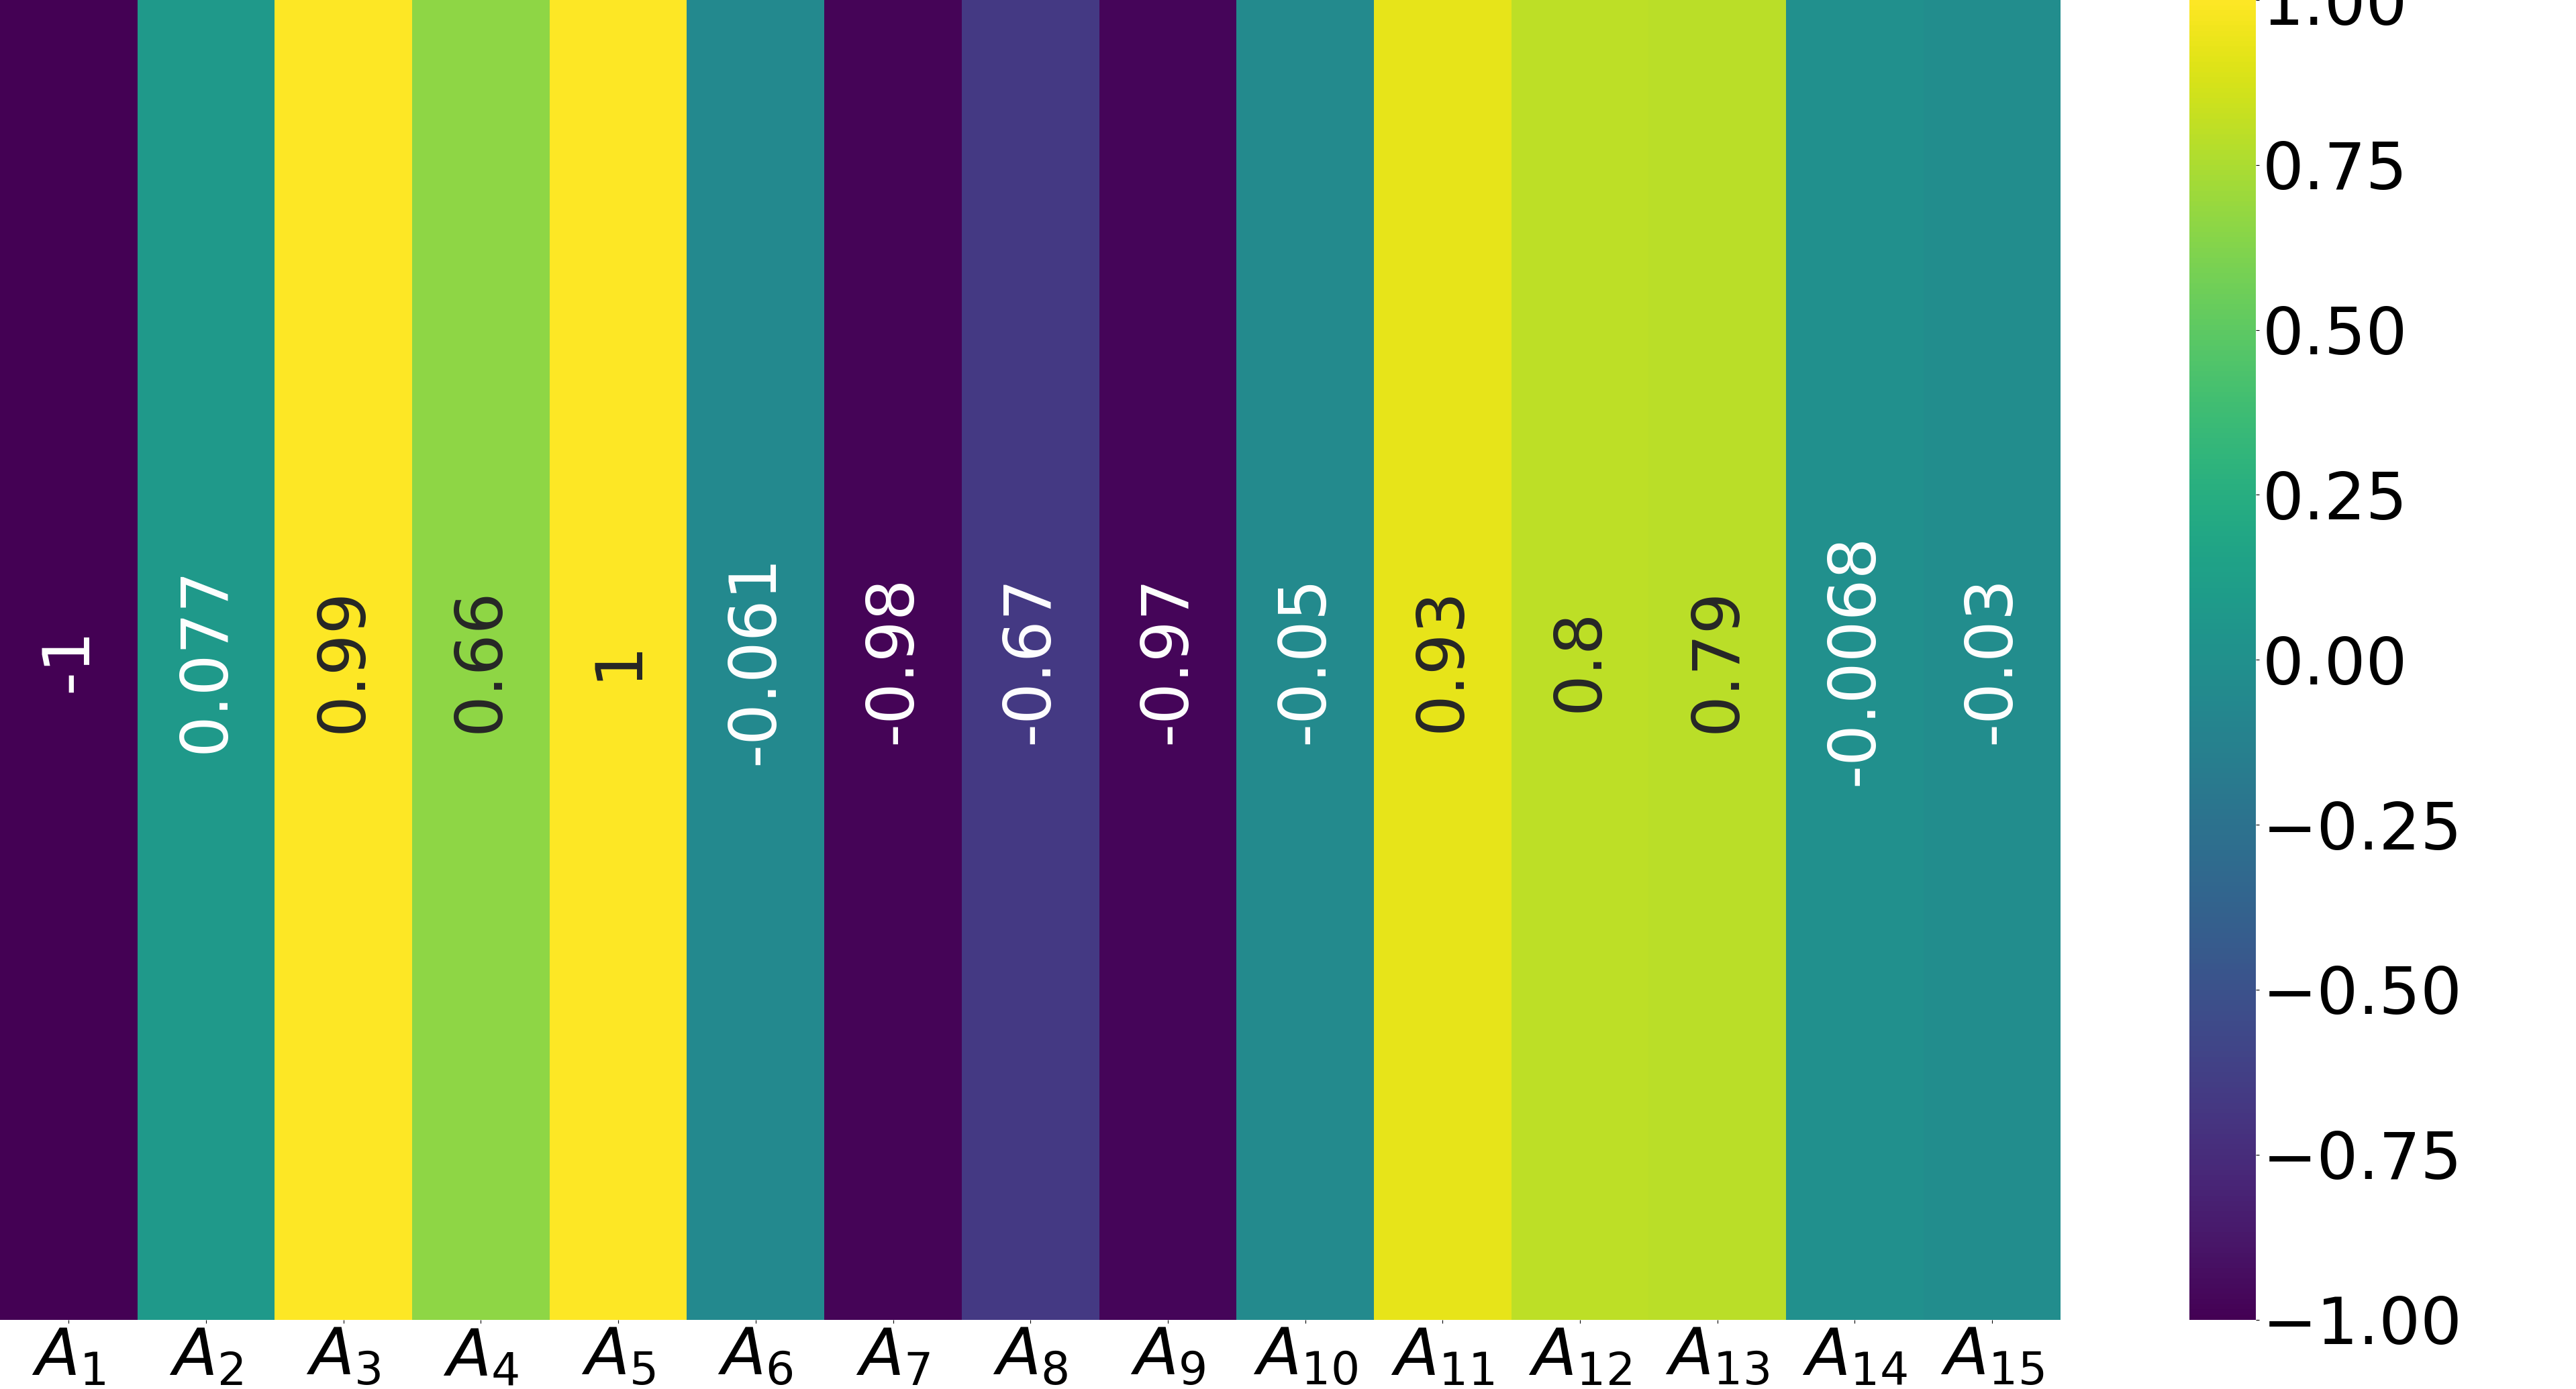
\includegraphics[width=\linewidth]{img/qlp_corr/An_coil0.png}
		\subcaption{Correlation with coil $0$}
	\end{subfigure}
	\begin{subfigure}{0.49\linewidth}
		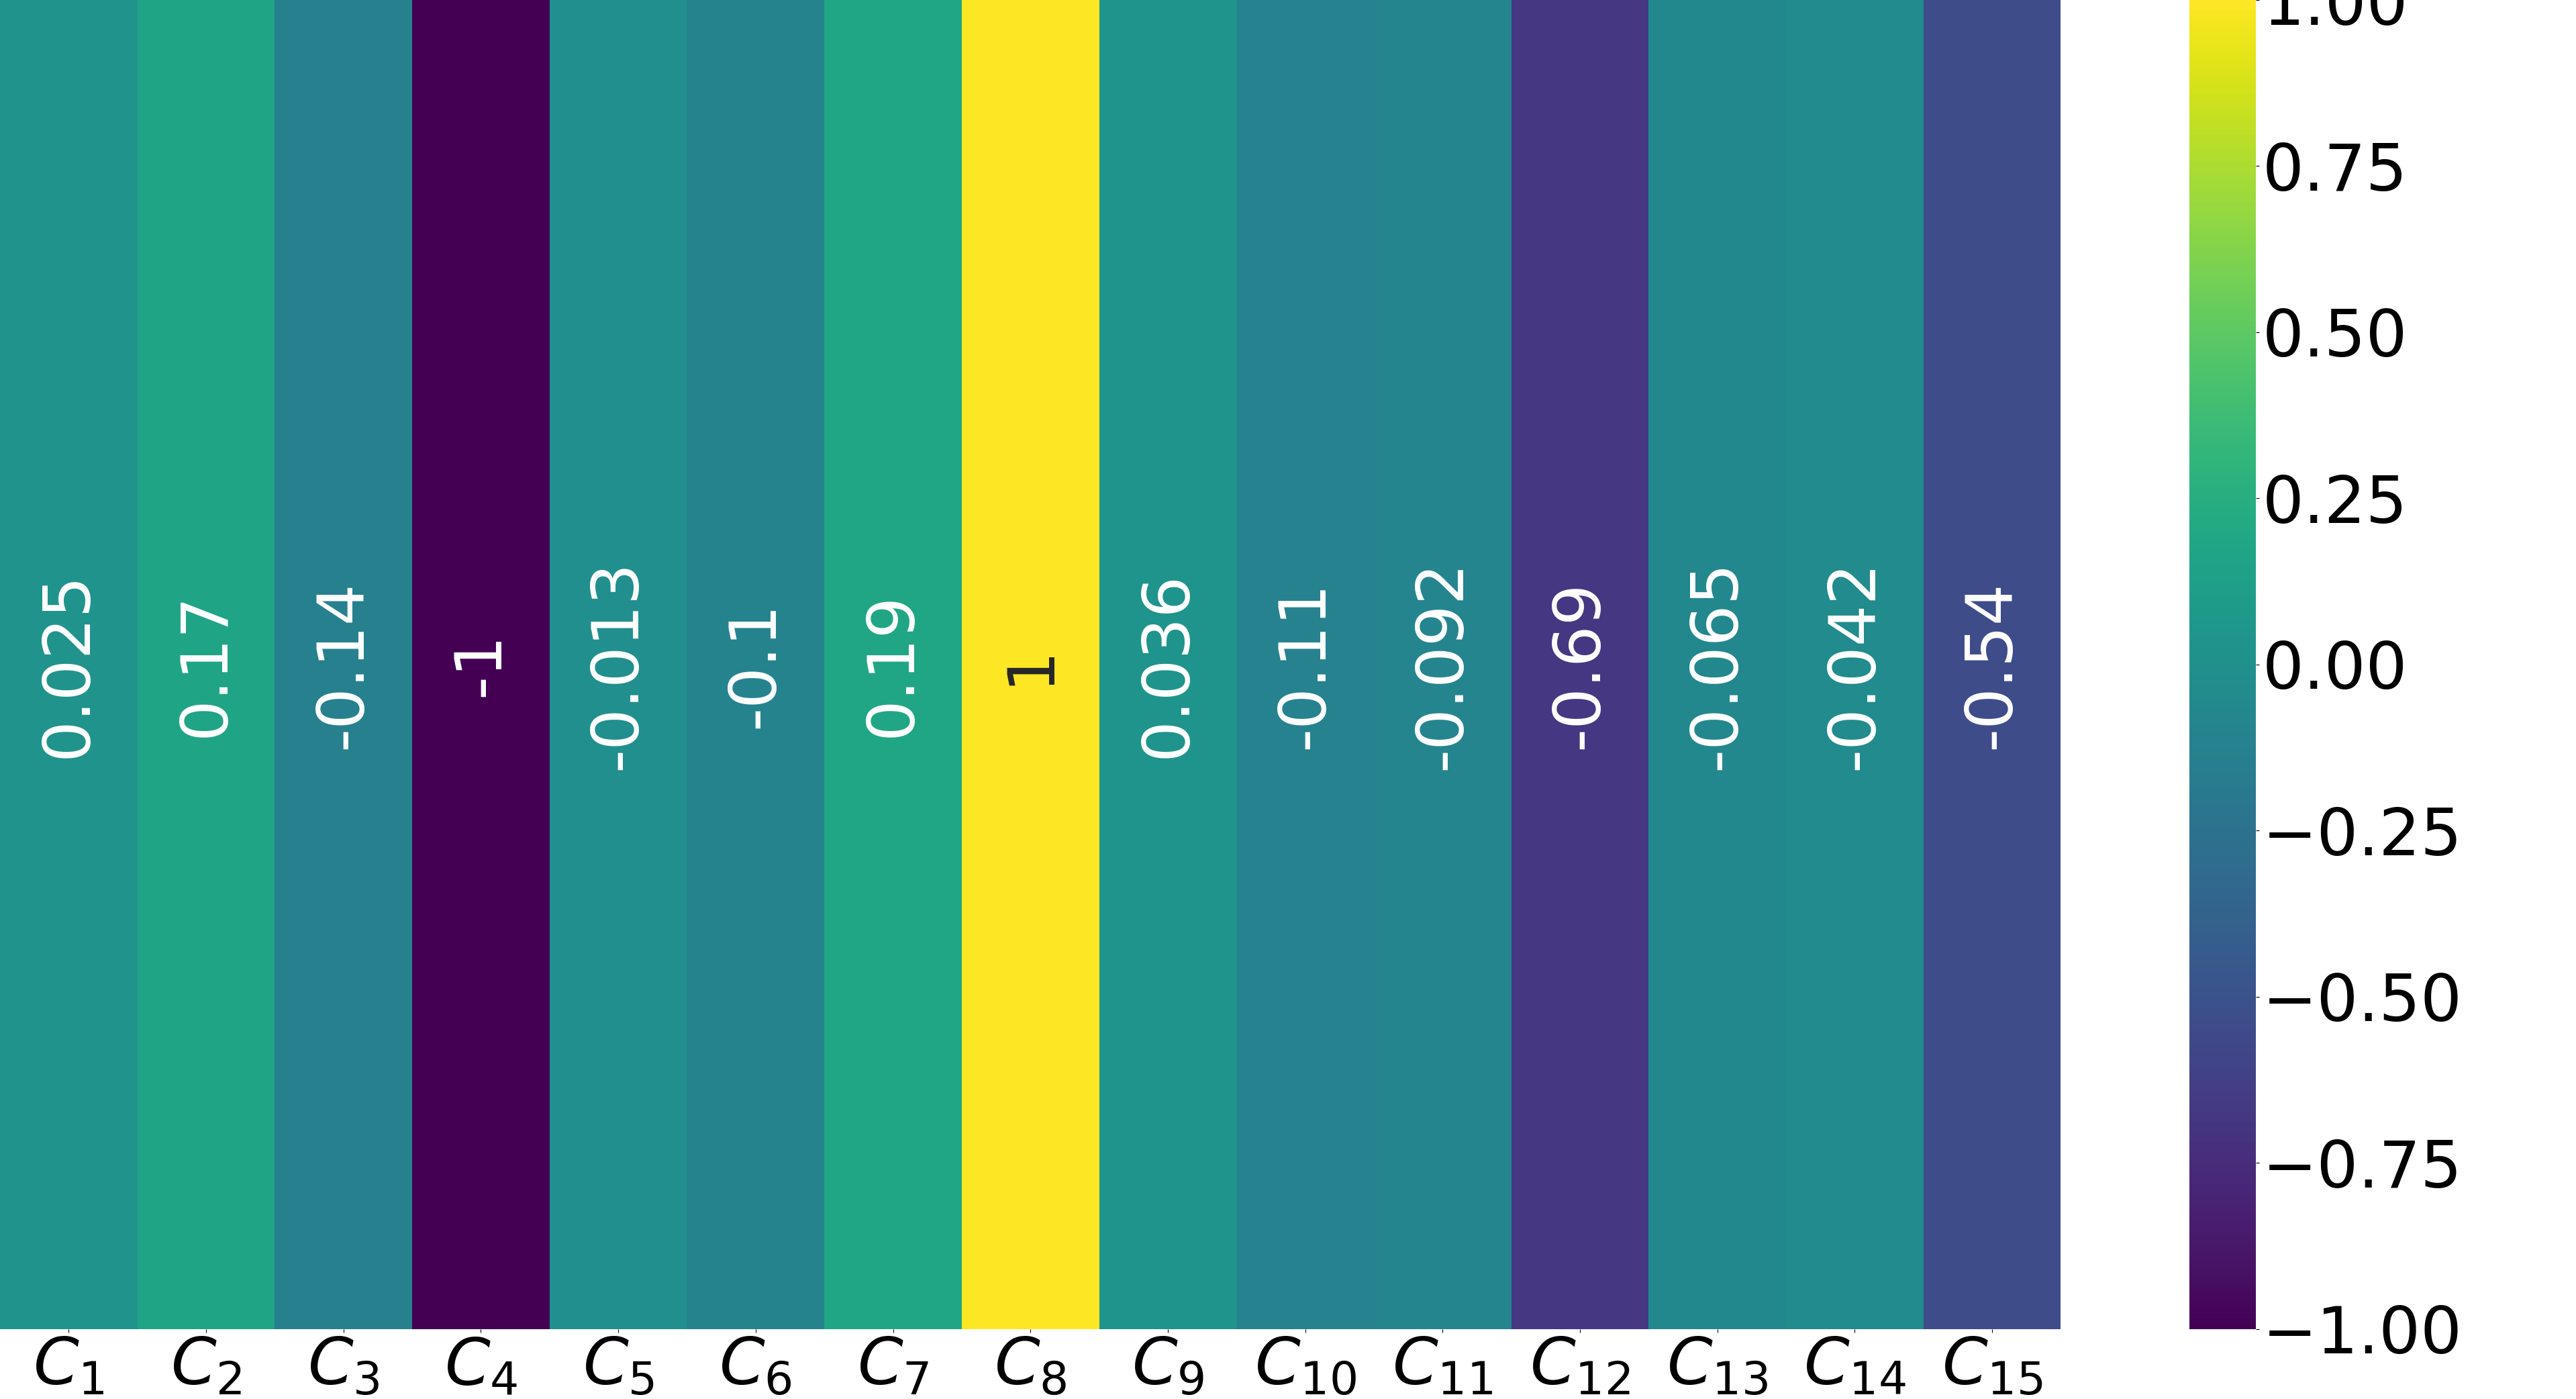
\includegraphics[width=\linewidth]{img/qlp_corr/An_coil1.png}
		\subcaption{Correlation with coil $1$}
	\end{subfigure}
	\begin{subfigure}{0.49\linewidth}
		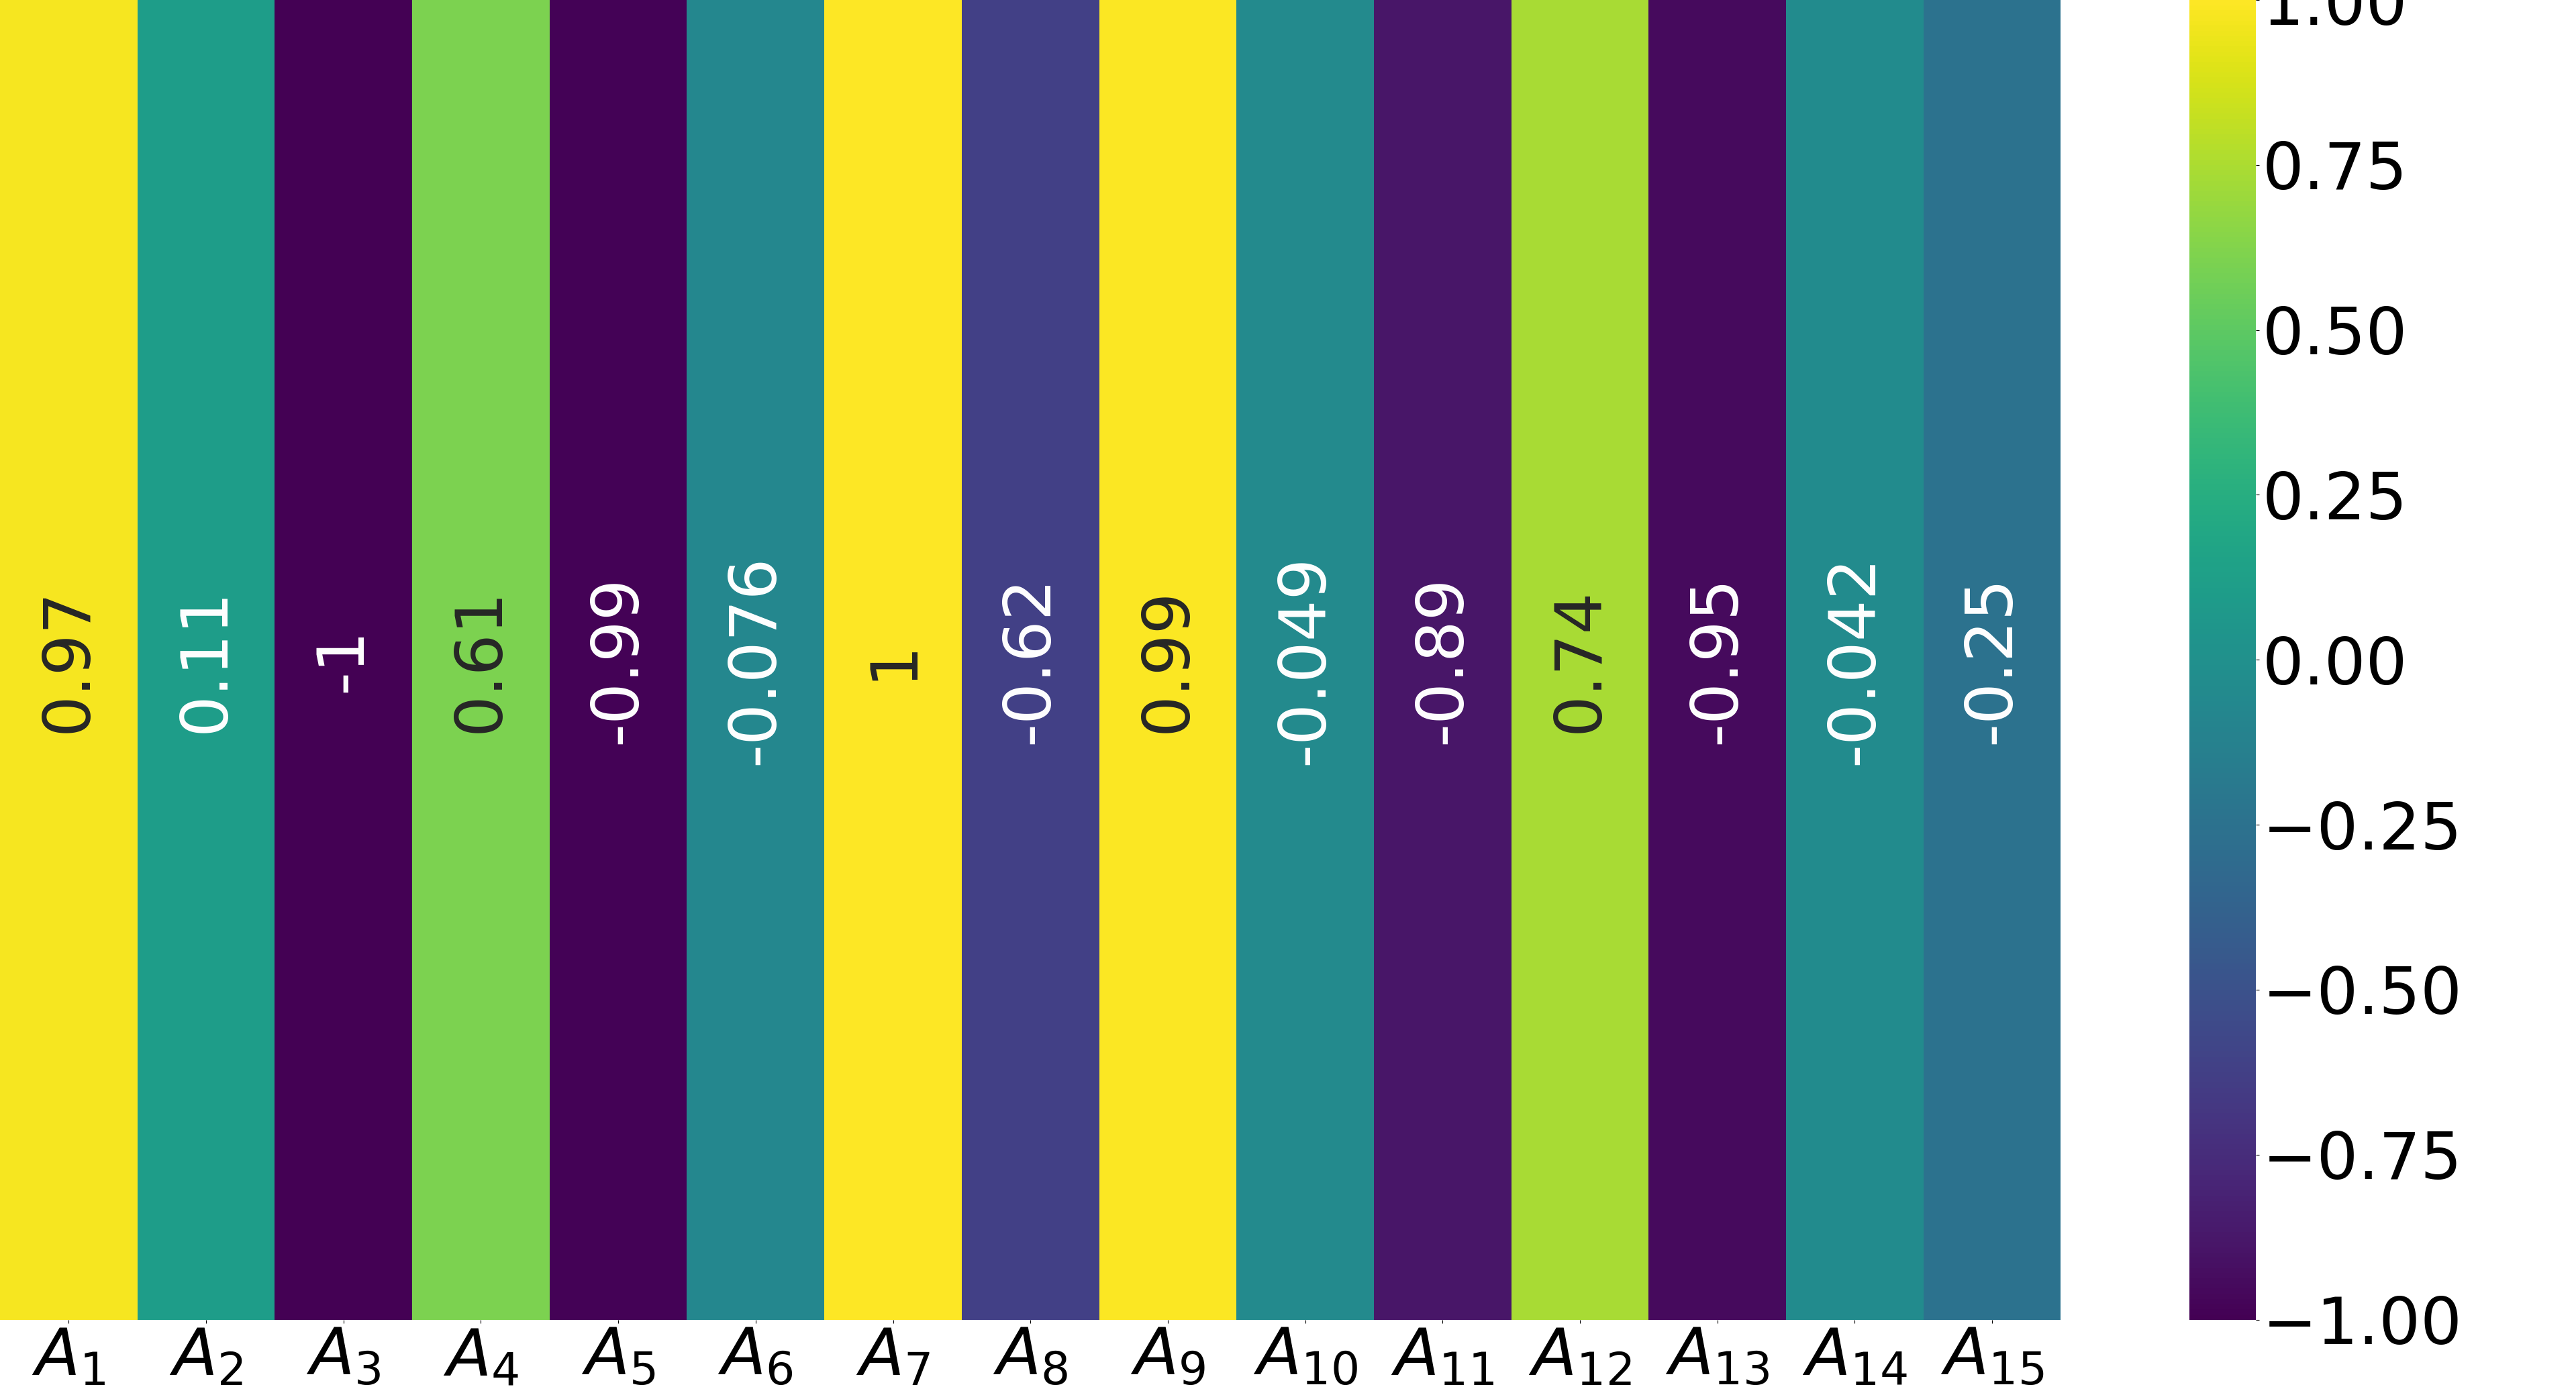
\includegraphics[width=\linewidth]{img/qlp_corr/An_coil2.png}
		\subcaption{Correlation with coil $2$}
	\end{subfigure}
	\begin{subfigure}{0.49\linewidth}
		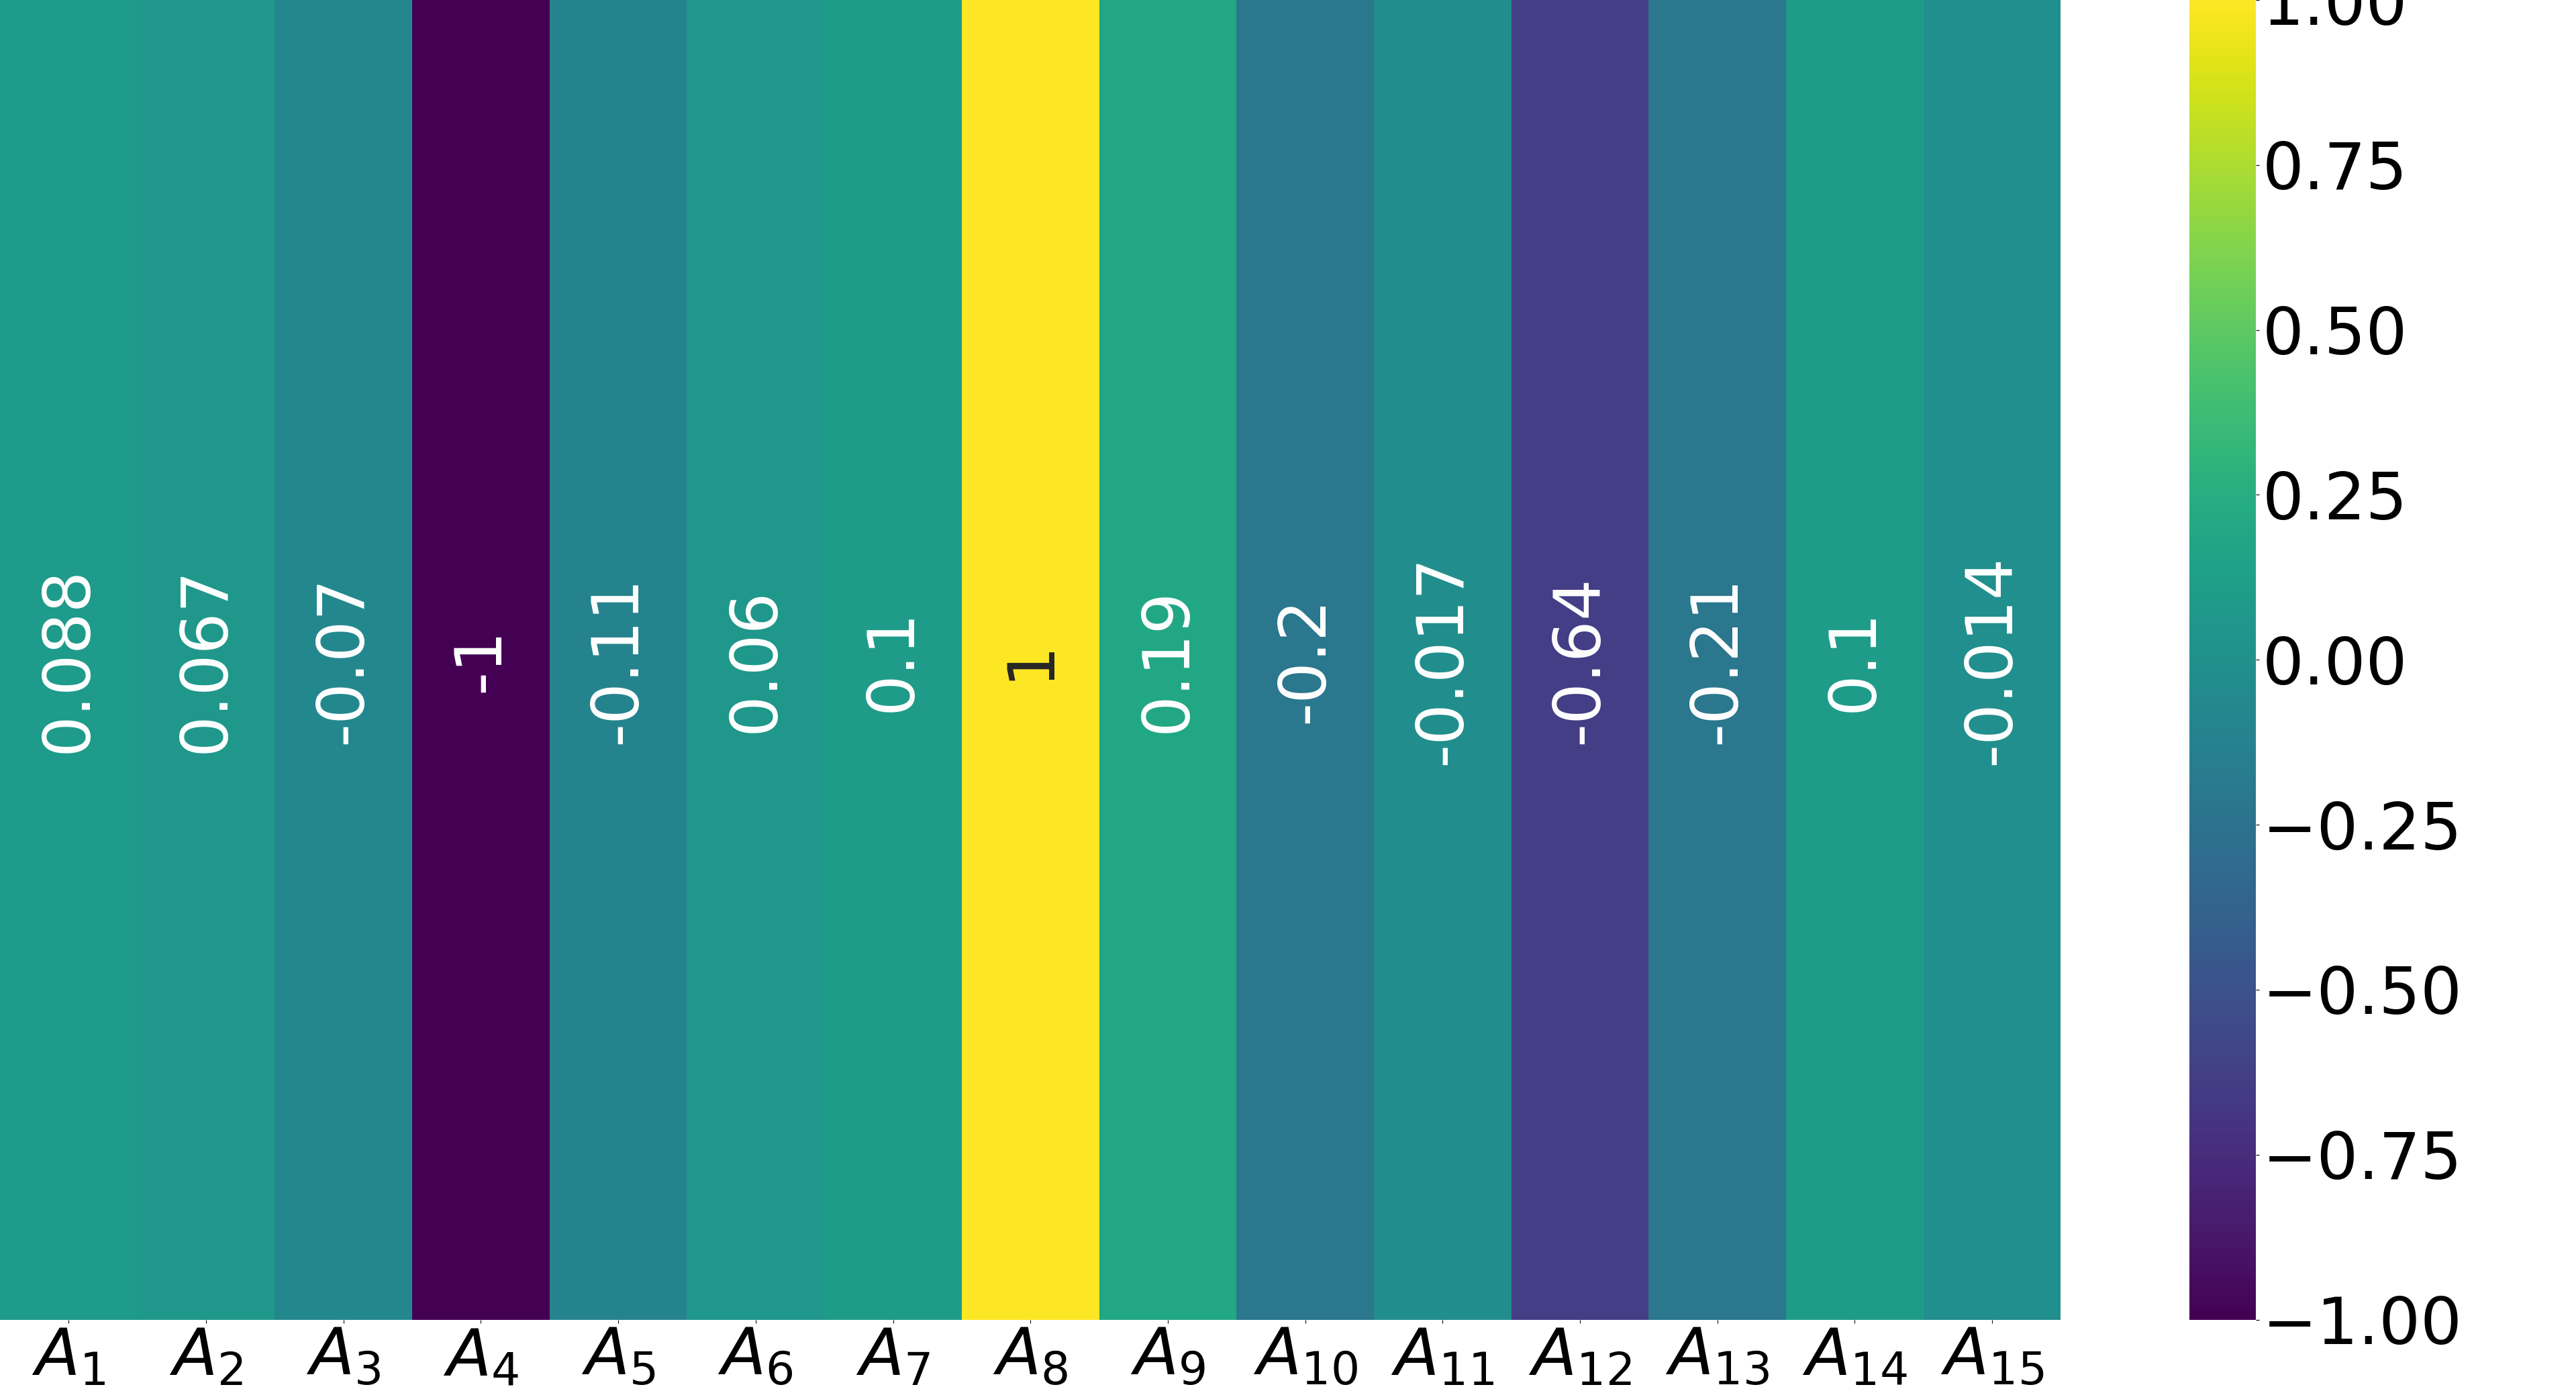
\includegraphics[width=\linewidth]{img/qlp_corr/An_coil3.png}
		\subcaption{Correlation with coil $3$}
	\end{subfigure}
	\caption{Correlation between the harmonics of the \an\ attribute and the labels for \qlp.}
	\label{fig:an-lcorr-qlp}
\end{figure}

\noindent If we remind ourselves of the correlation existing among the harmonics (cfr. \Cref{fig:an-corr}), we can see that:
\begin{itemize}
	\item Contrarily to what we discovered in \Cref{sec:qrp-preprocessing}, \an[2]\ is not
	      fundamental to explain the expected results;
	\item the harmonics containing more information are the odd ones (\an[1], \an[3], \an[5],
	      \ldots); this means that we will be able to only take one from the bunch, due to the
	      strong correlation originally identified among odd-numbered harmonics (see
		\Cref{fig:an-corr} and \Cref{sec:an}).
\end{itemize}
A potential dataset could be constructed using a primary odd harmonic (like \an[1]\ or \an[3]), the
harmonic performing the best among \an[4], \an[8]\ and \an[12]\ (which are all strongly correlated,
see \Cref{sec:an}), and finally, \an[2]\ and another high-order harmonic could be beneficial. While
the model is clearly suited to explain the behavior of coils $0$ and $2$, we thought it wise to
look for an alternative to explain the behavior of coils $1$ and $3$.
\begin{figure}[!ht]
	% Font size = 40
	\centering
	\begin{subfigure}{0.6\linewidth}
		\centering
		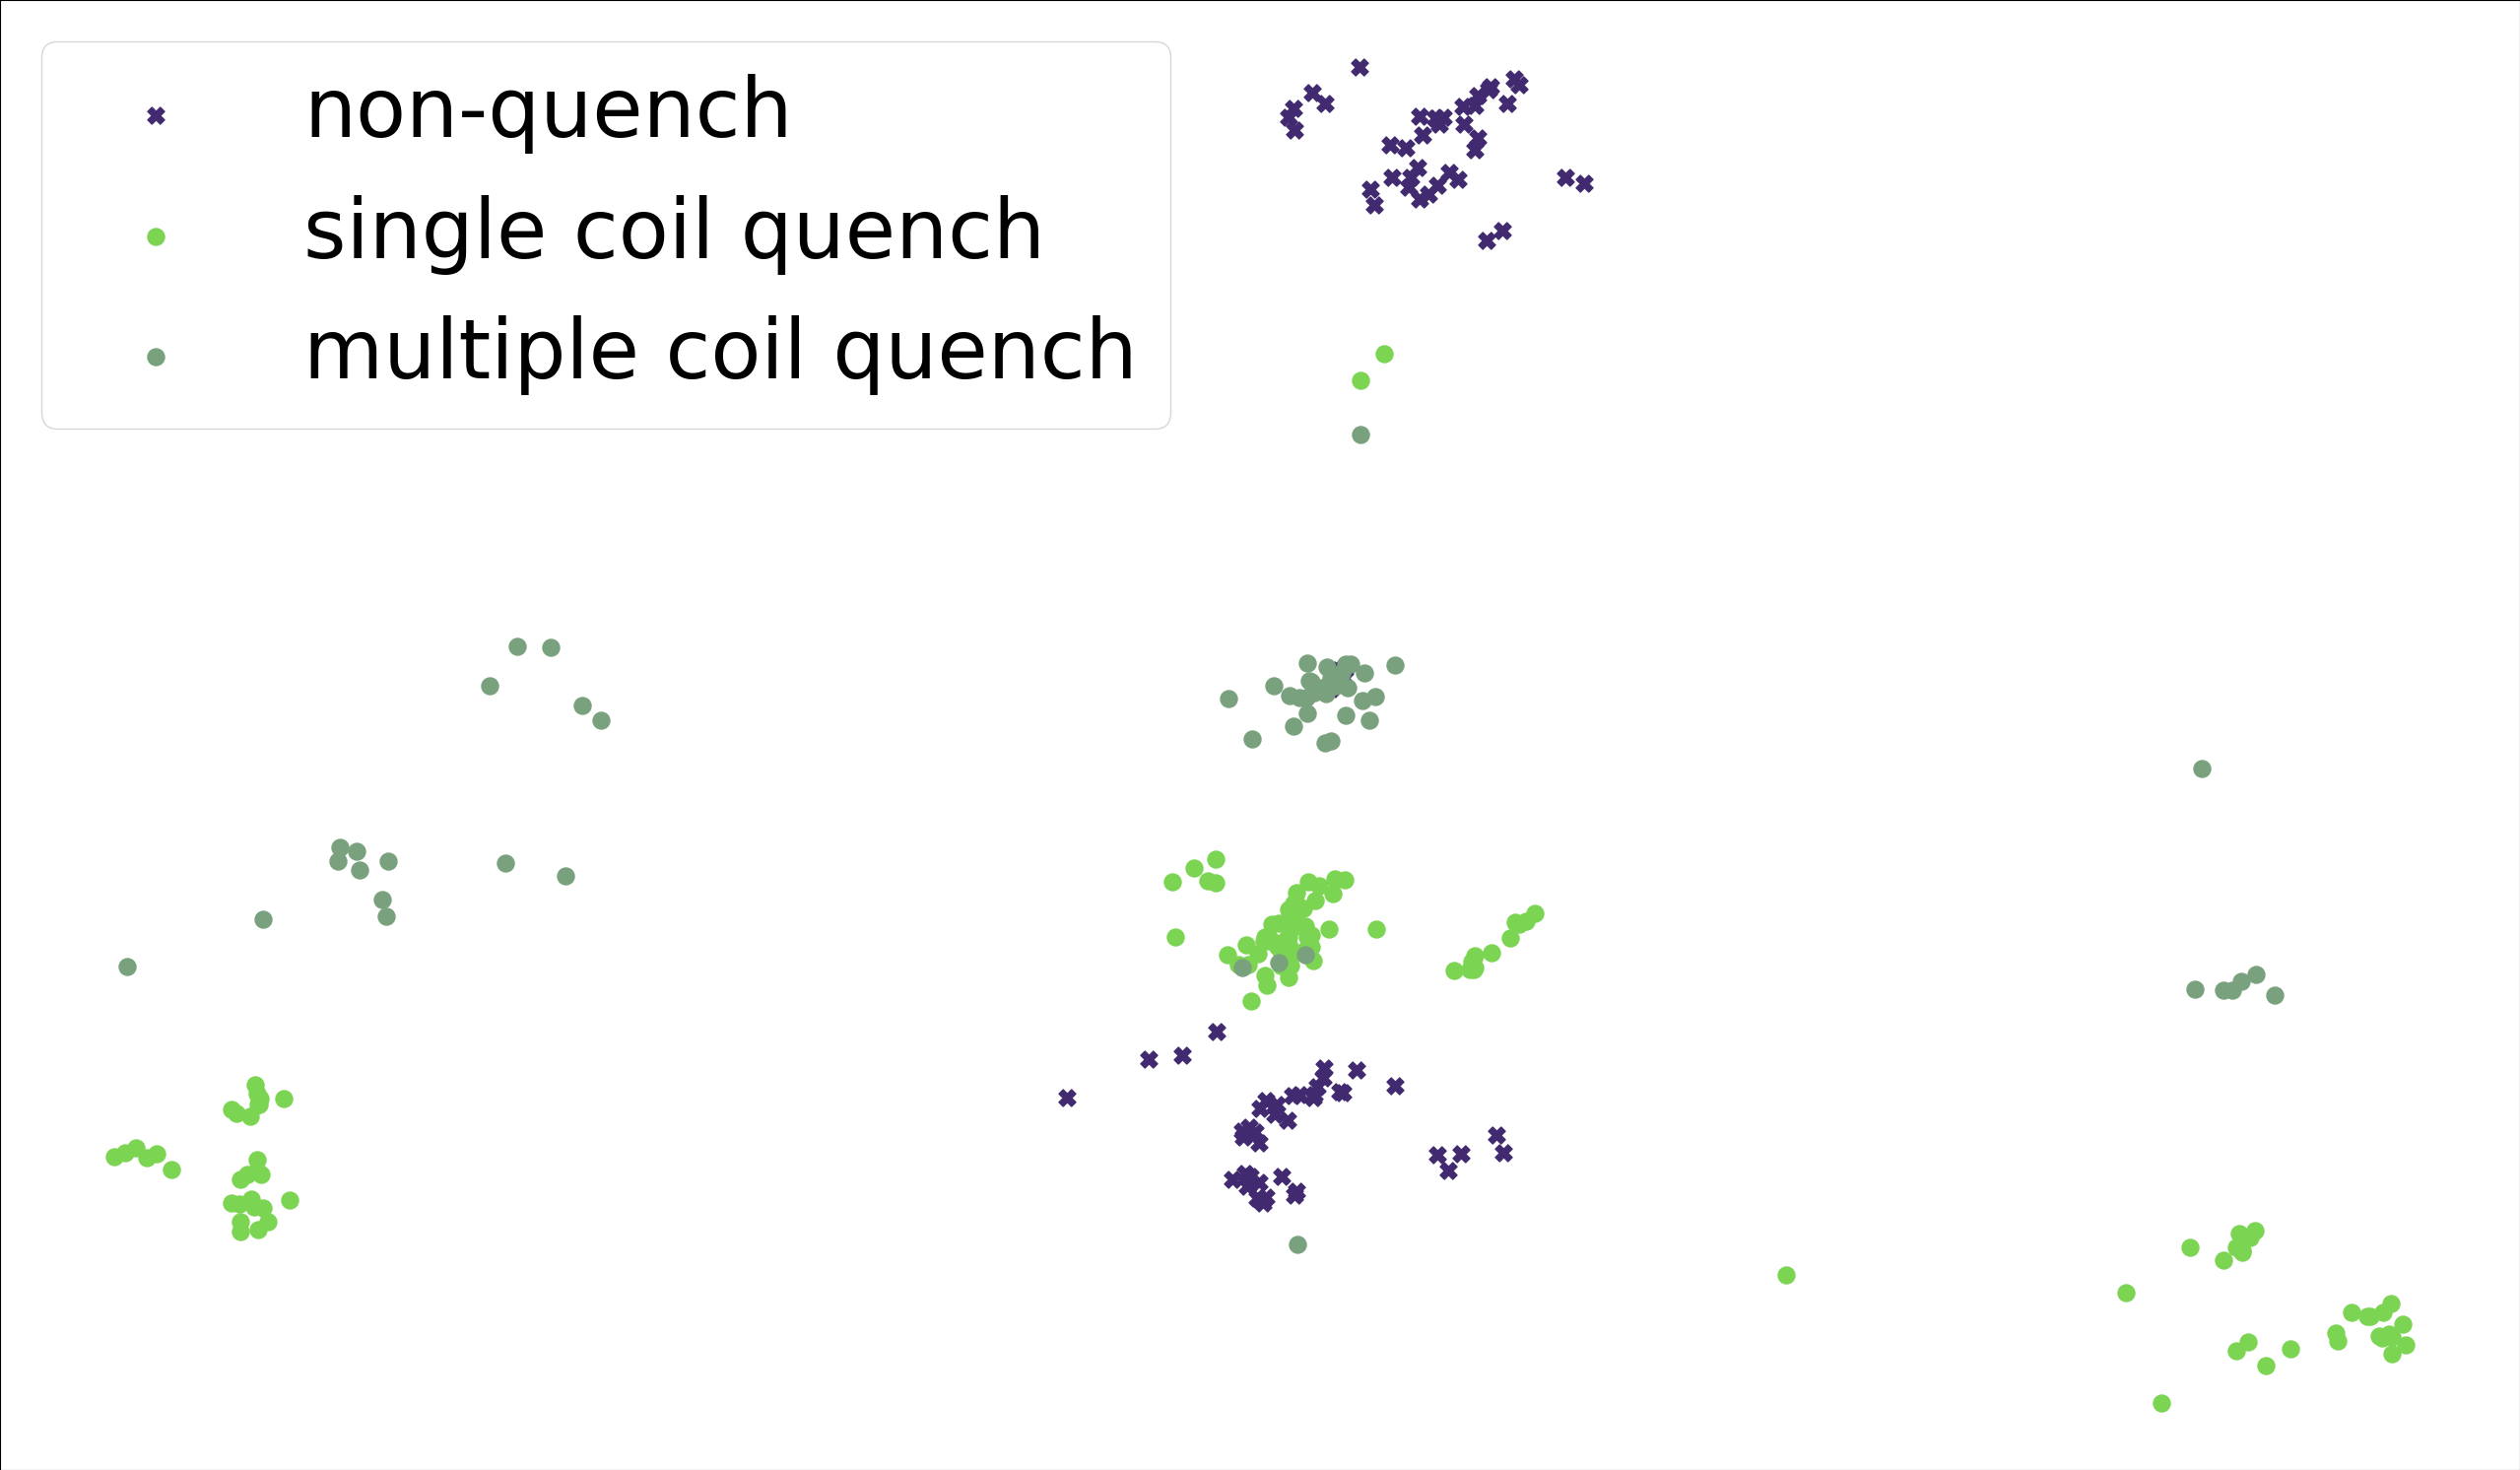
\includegraphics[width=\linewidth]{img/quench_dist_qlp/single_vs_multiple_An.png}
		\subcaption{}
	\end{subfigure}
	\begin{subfigure}{0.6\linewidth}
		\centering
		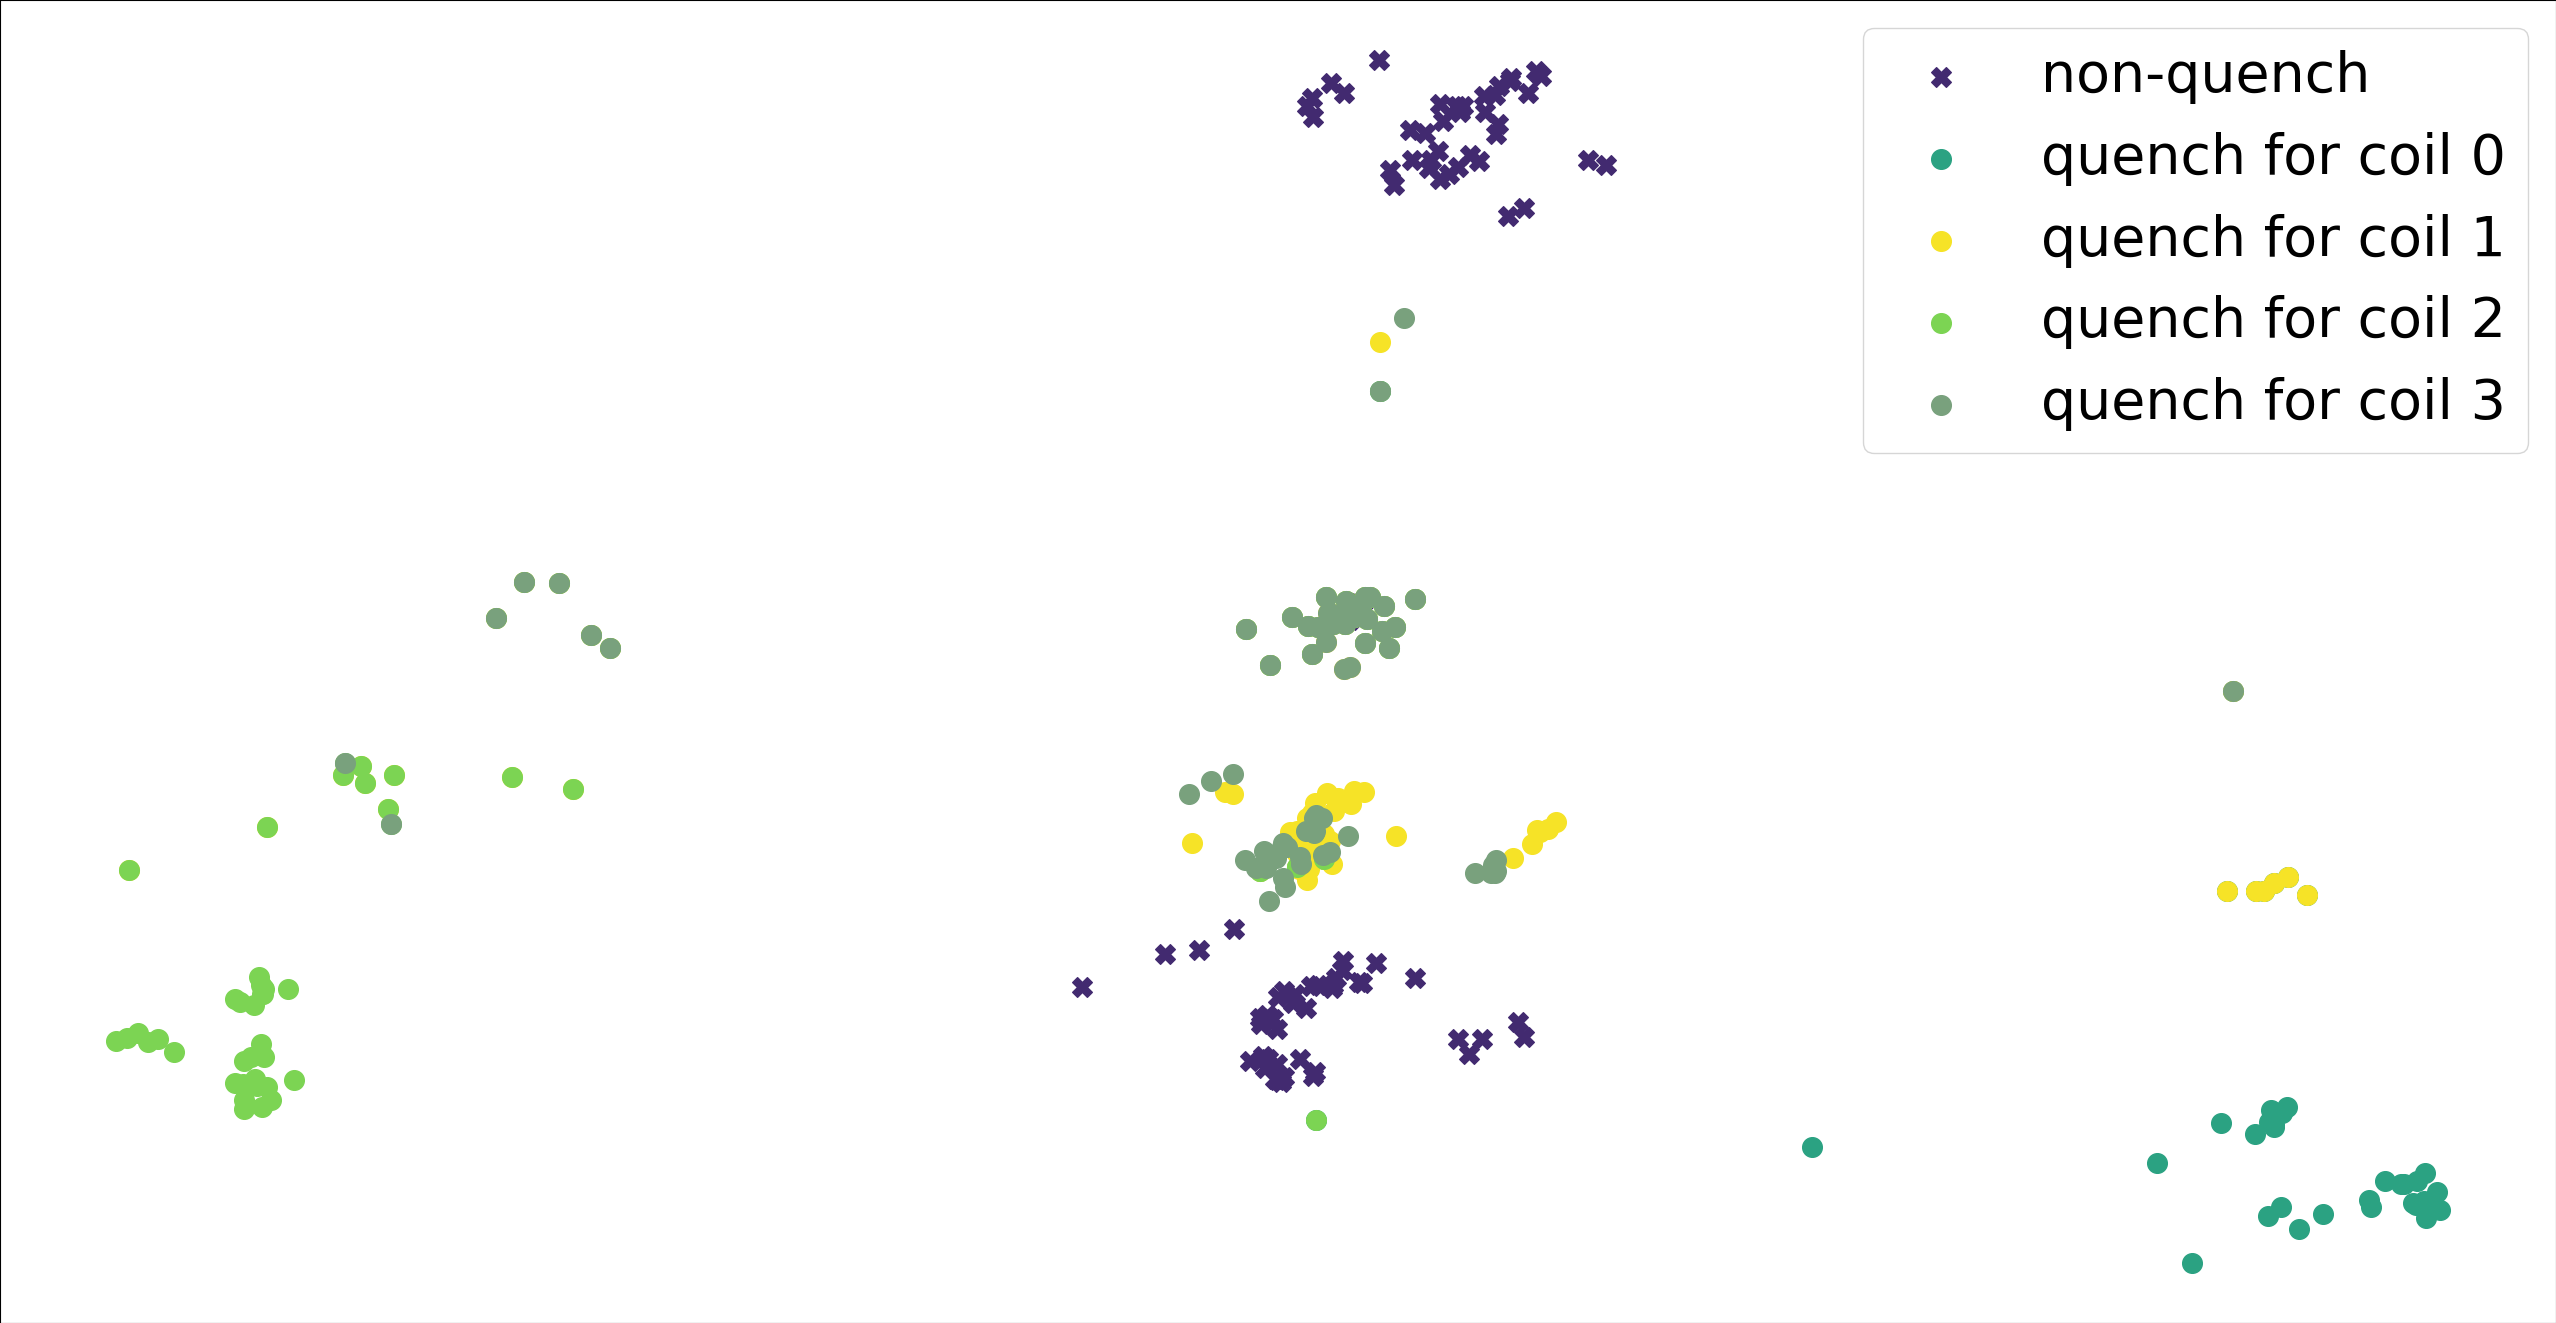
\includegraphics[width=\linewidth]{img/quench_dist_qlp_an.png}
		\subcaption{}
	\end{subfigure}
	\caption{Visualization of the \an\ attribute, the data was plotted after a run of \pca\
		dimensionality reduction. Sub-figure (a) highlights the samples based on how many quenches
		are associated to the specific sample $\{0, 1, \text{many}\}$. Sub-figure (b) highlights the
		samples based on the specific coil quenched $\{\text{None}, 0, 1, 2, 3\}$.}\label{fig:an-coilq-dist}
\end{figure}

In \Cref{fig:an-coilq-dist} we visualized the distribution of samples for \an\ in
bidimensional space, after a round of \pca\ dimensionality reduction (moving from $15$ to $2$
dimensions). Sub-figure (a) labels data based on the number of quenched coils associated to the
sample. We can evidently identify a series of clusters, characterized by a high degree of purity;
(and we had already noticed this behavior in \Cref{sec:an} on different labels). In
\Cref{sec:qlp-cluster} we are going to discuss the clustering approach on this specific attribute.
In sub-figure (b), we labelled the data based on which coil was quenched. The division of the labels
is not as neat as in sub-figure (a), which lead us to think that clustering could be used as a
preprocessing step to then have another machine learning model work on the clustered data to predict
quench localization.

While sub-figure (b) doesn't tell us everything we need to know, we can see that coil $1$ and coil
$3$ are fairly mixed together, furthermore both of them are usually involved in multi-coil quenches.
These hints are giving us another possible reason why \an\ is less-than-ideal to
predict quench localization on coils $3$ and $1$ \Cref{fig:an-lcorr-qlp}.

\subsubsection{\bn}
While experimenting with \qrp, we discovered that \bn\ was the attribute that performed the least
among the ones available. We didn't expect similar results from \qlp\ because, after the analysis
done in \Cref{chp:problem} we hypothesized that: \emph{if} \an\ performance are actually good for coils $0$
and $2$ (which are the horizontal coils), then \bn\ \emph{should} be able to explain the behavior of
the vertical coils ($1$ and $3$)~\footnote{
	Let us be reminded that the harmonics of magnetic field are dependent on the harmonic
	coefficient:
	\[C_n = B_n + iA_n \enspace.\]
	The two components of $C_n$ are the \emph{skew} component, \an, generating the horizontal
	fields, and the \emph{right} or \emph{normal} component, \bn, generating the vertical
	fields.
}.

\begin{figure}[!ht]
	% Font size = 70
	\centering
	\begin{subfigure}{0.49\linewidth}
		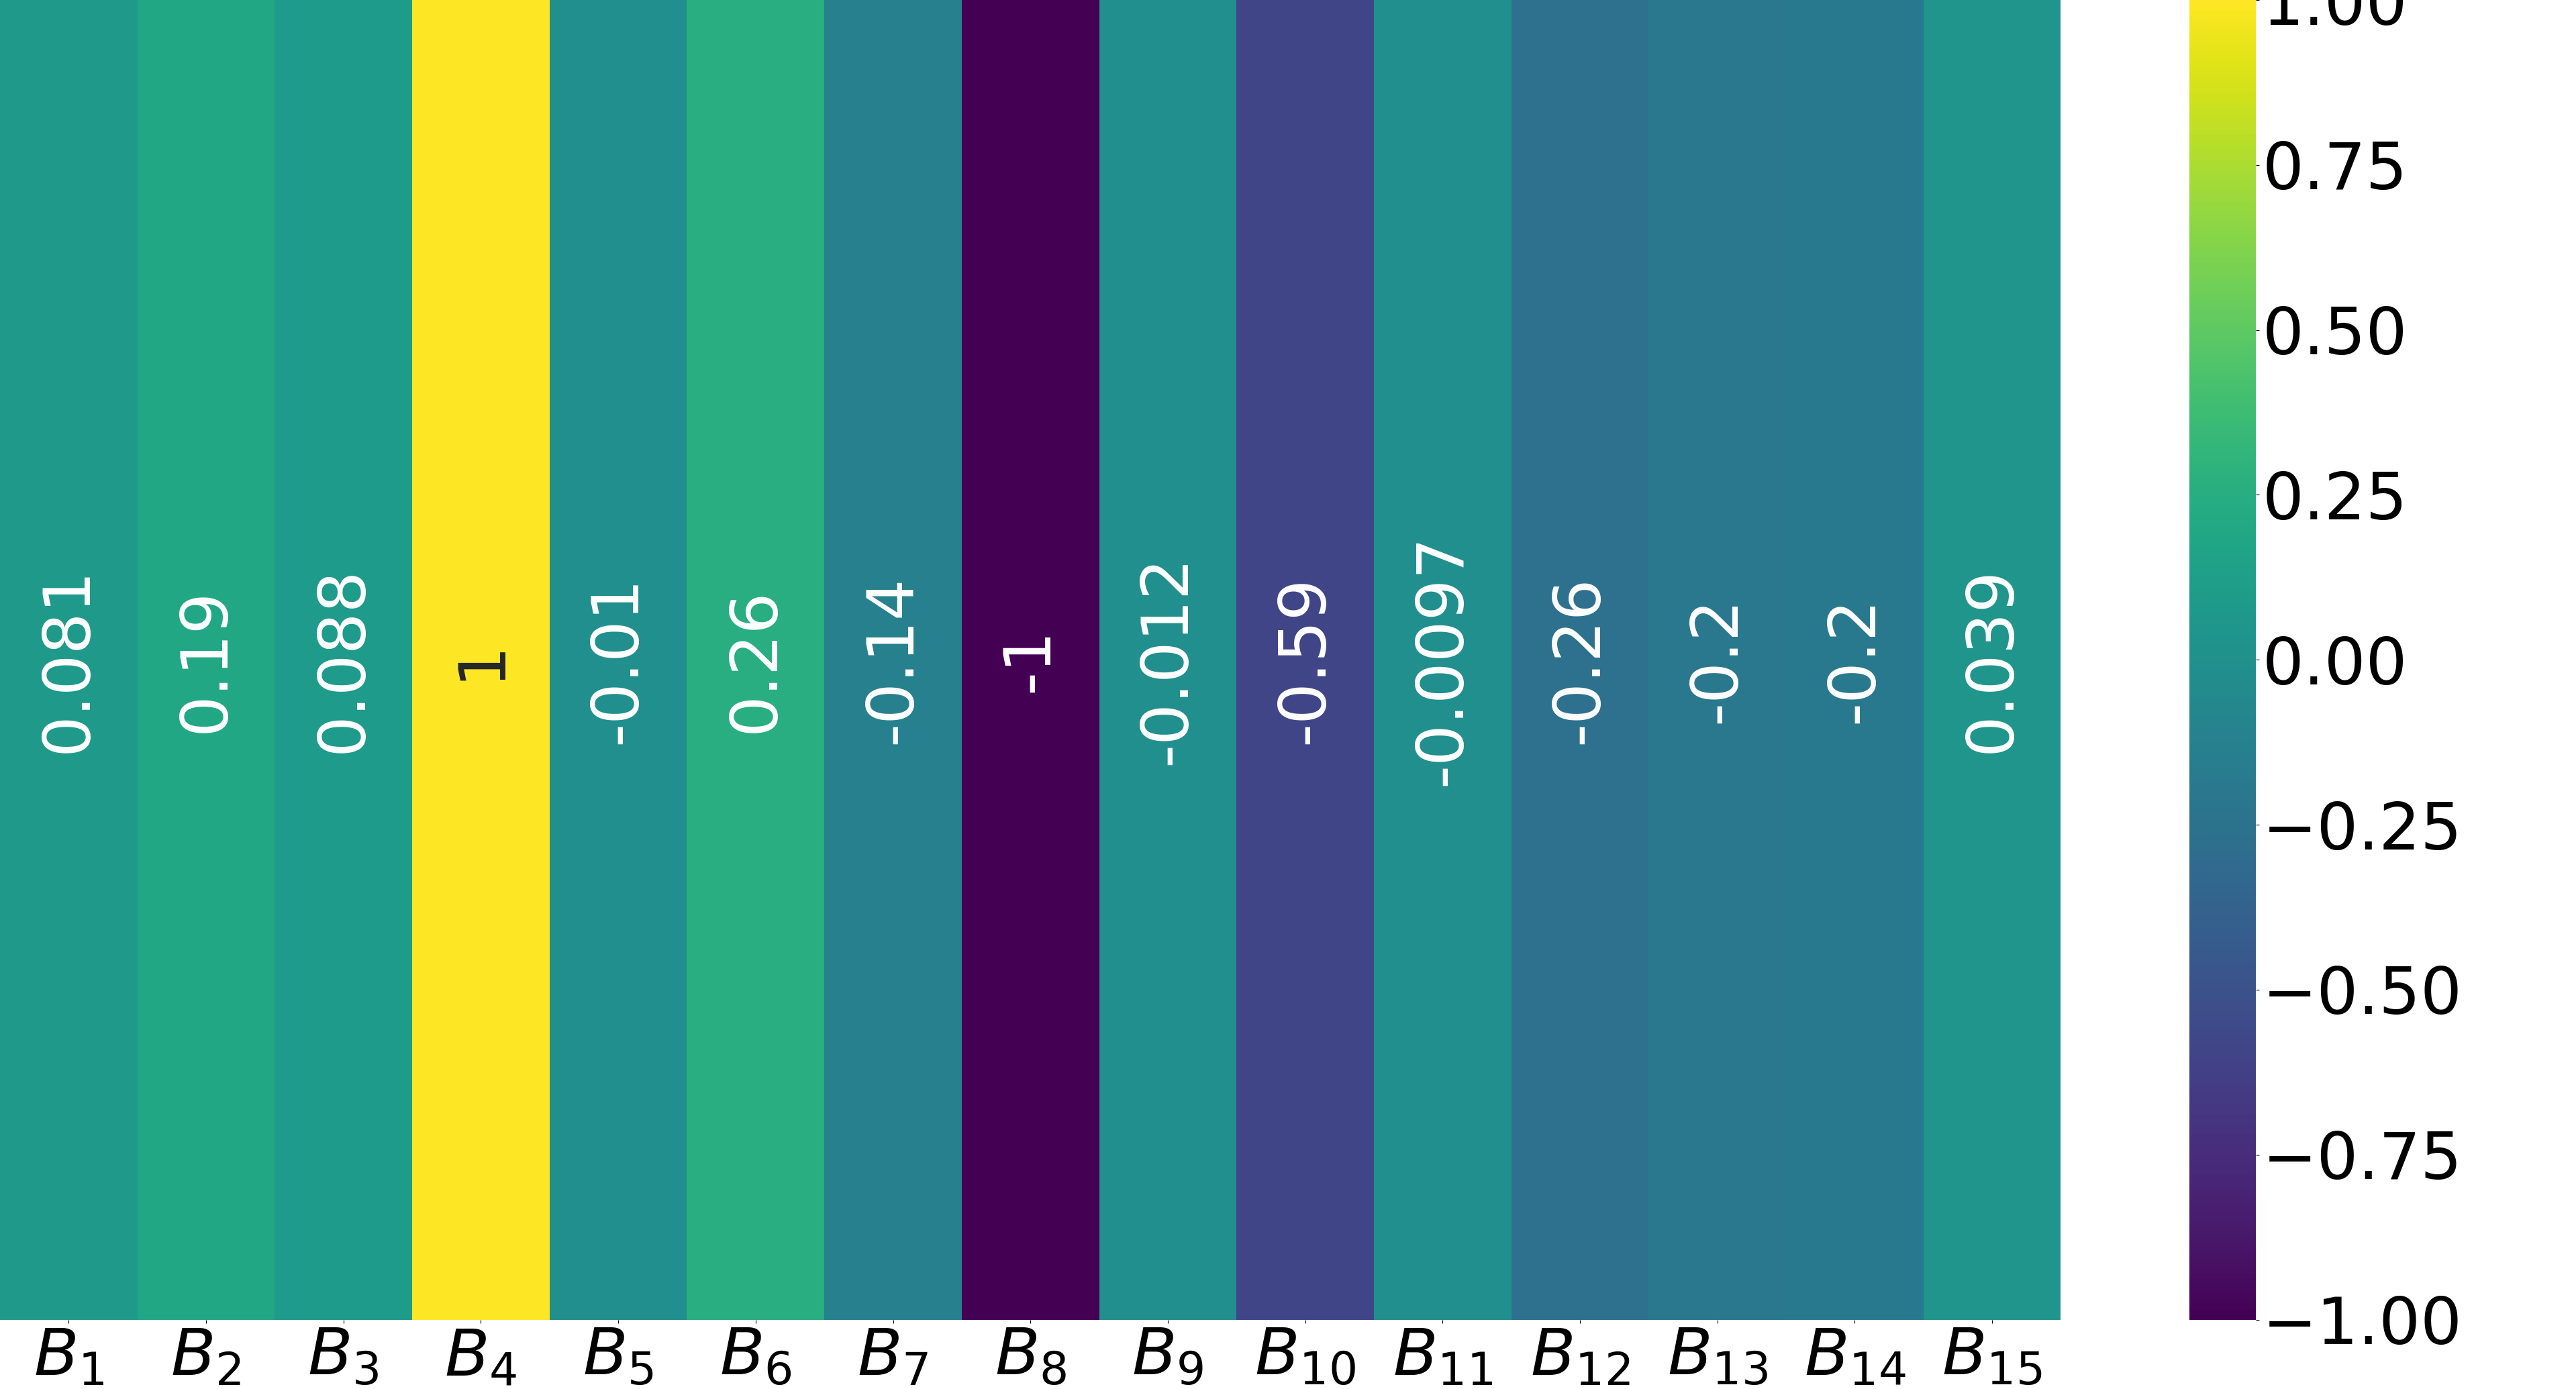
\includegraphics[width=\linewidth]{img/qlp_corr/Bn_coil0.png}
		\subcaption{Correlation with coil $0$}
	\end{subfigure}
	\begin{subfigure}{0.49\linewidth}
		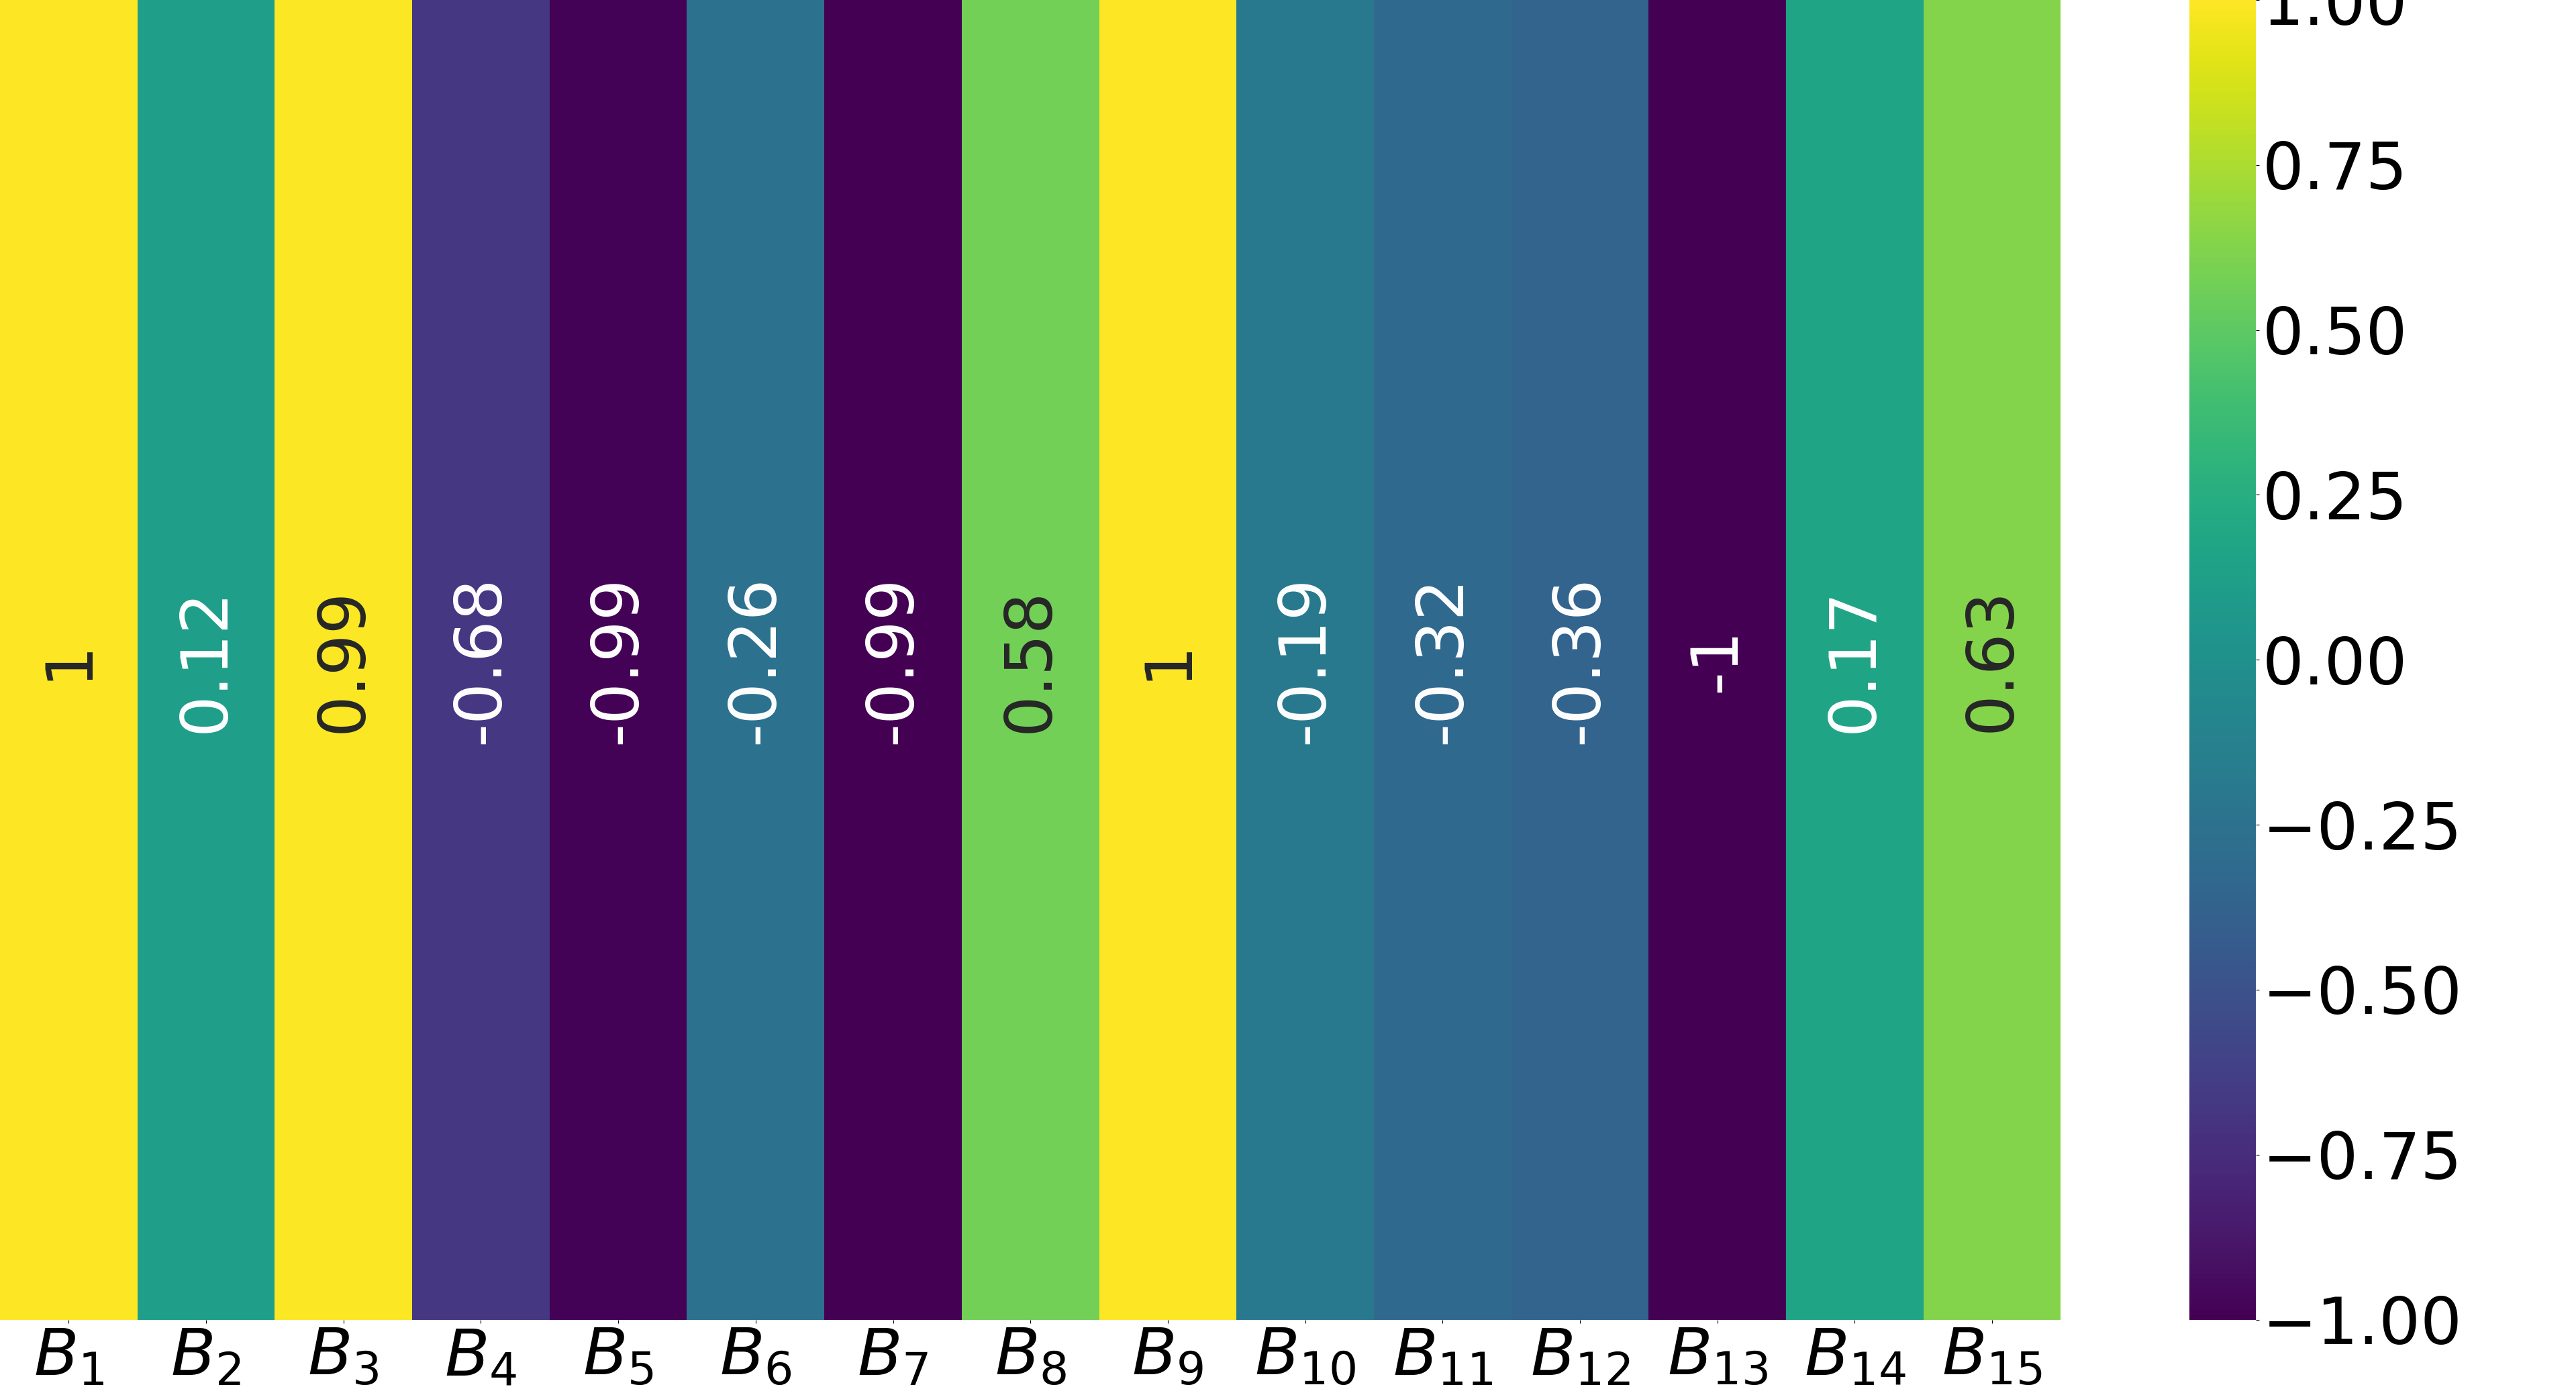
\includegraphics[width=\linewidth]{img/qlp_corr/Bn_coil1.png}
		\subcaption{Correlation with coil $1$}
	\end{subfigure}
	\begin{subfigure}{0.49\linewidth}
		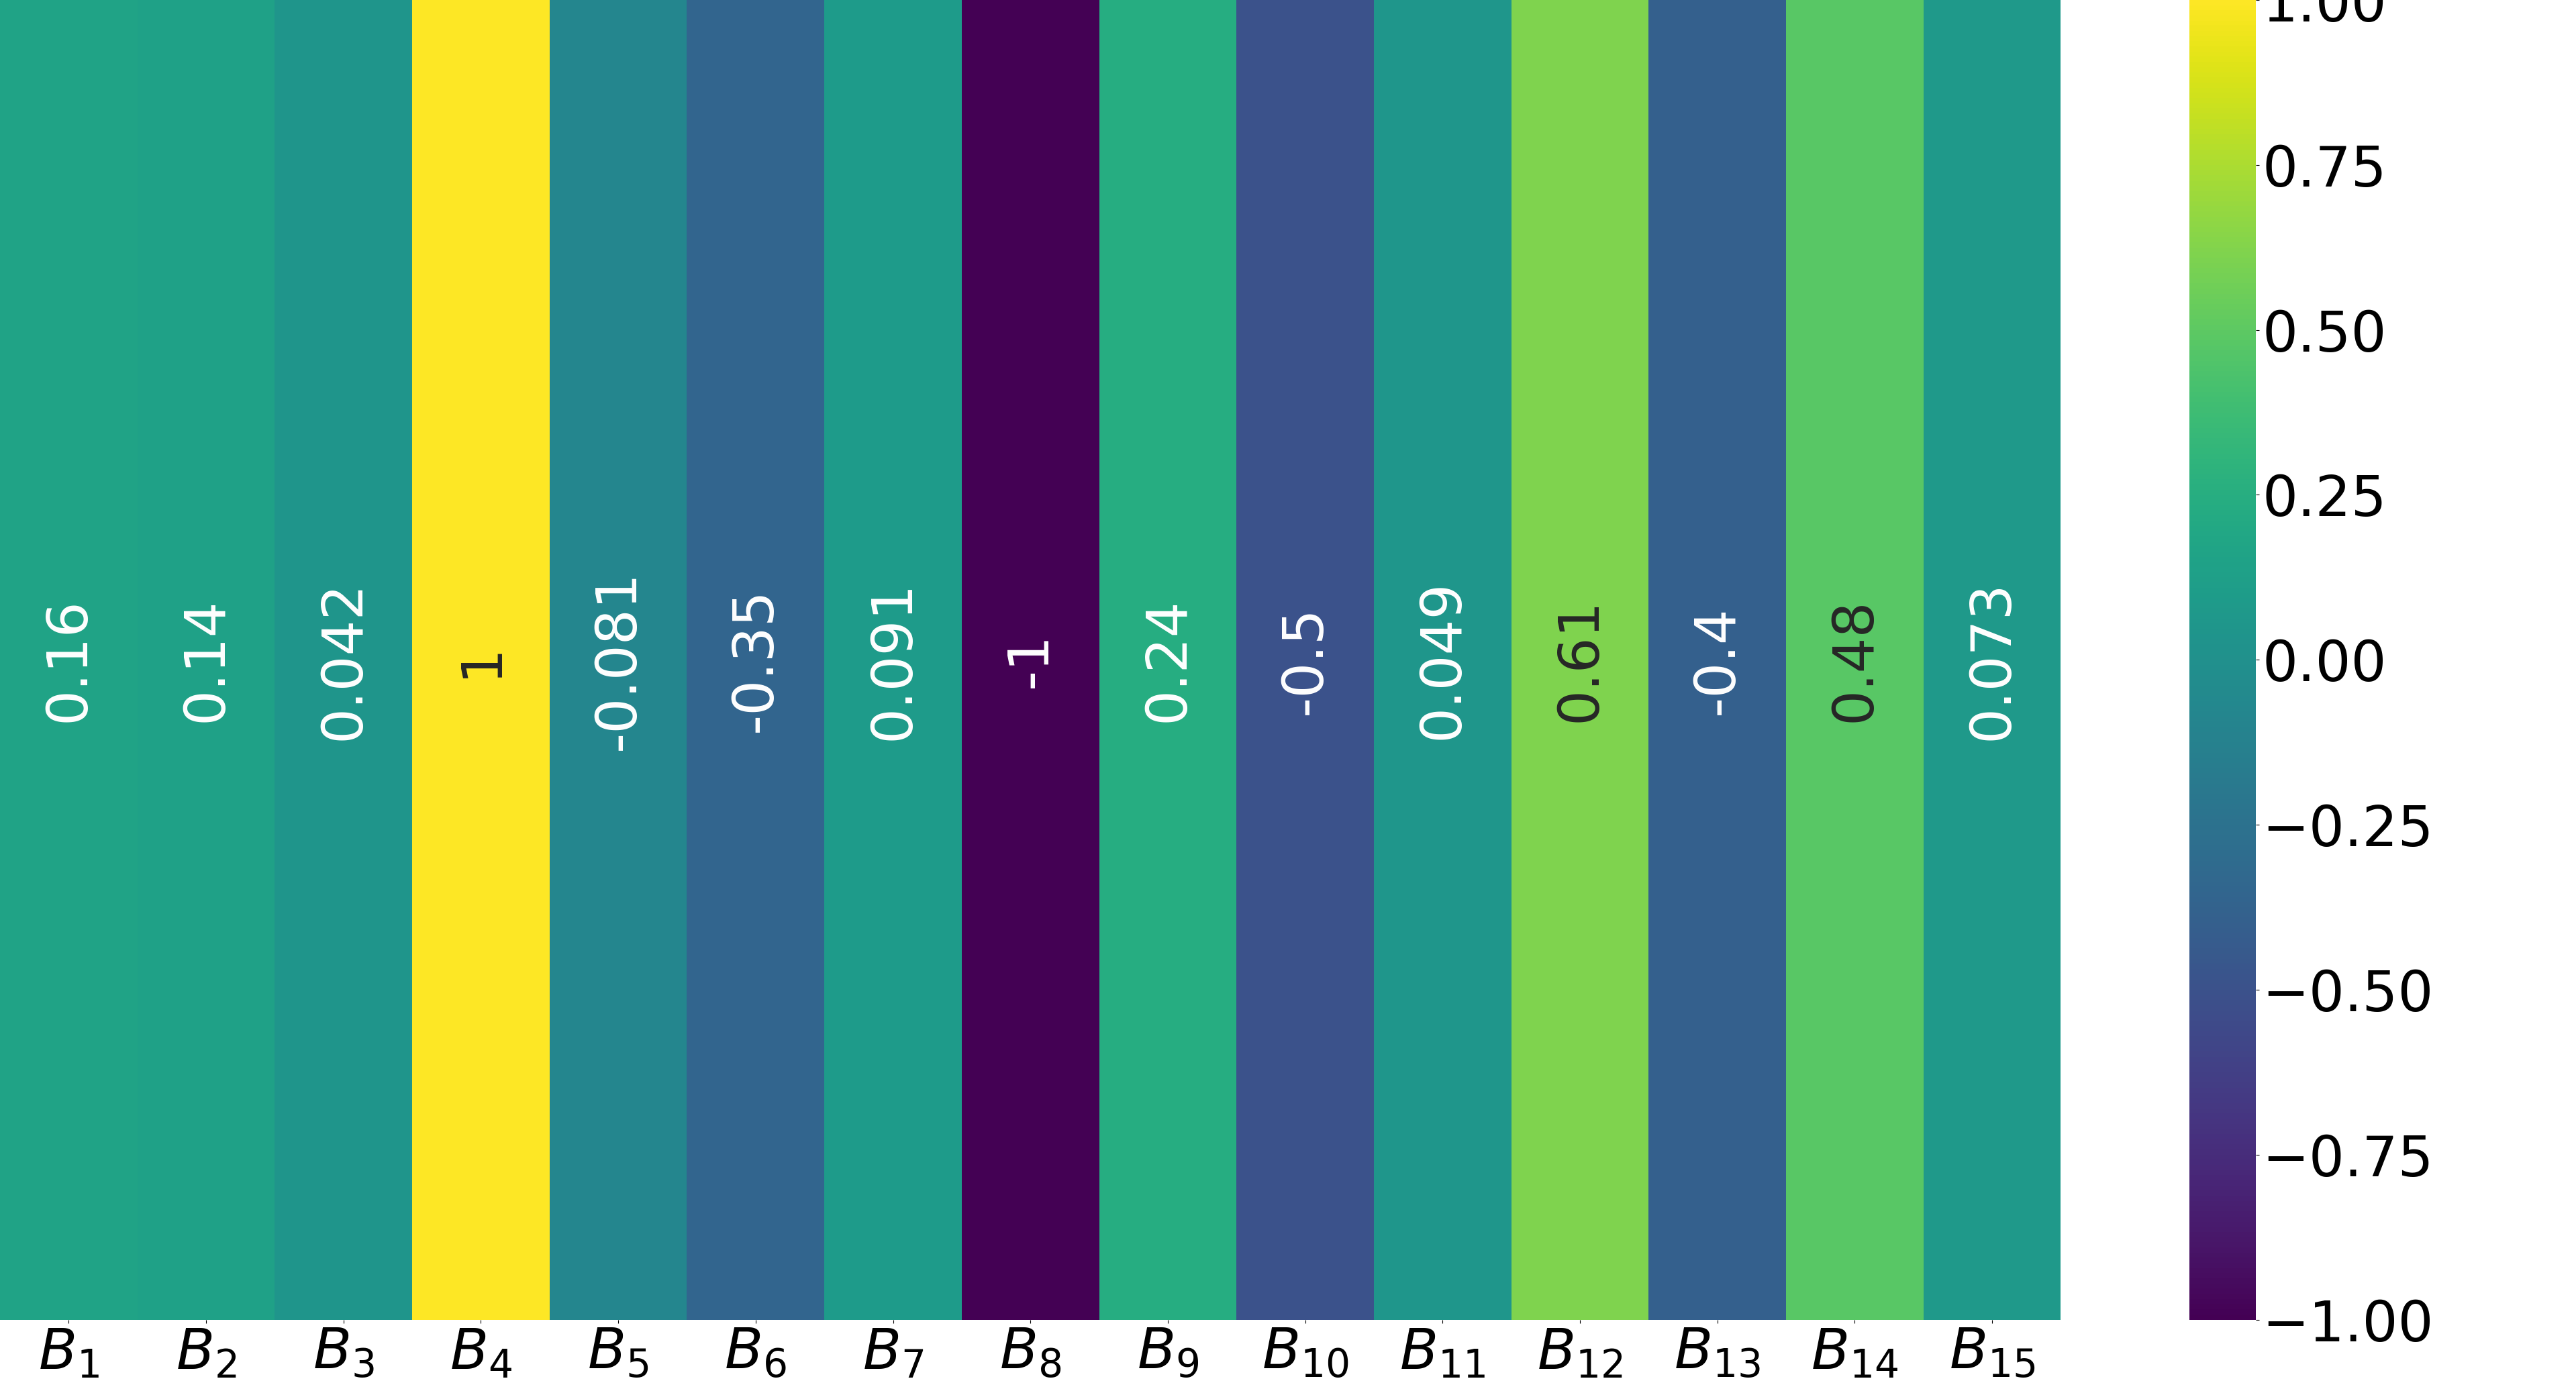
\includegraphics[width=\linewidth]{img/qlp_corr/Bn_coil2.png}
		\subcaption{Correlation with coil $2$}
	\end{subfigure}
	\begin{subfigure}{0.49\linewidth}
		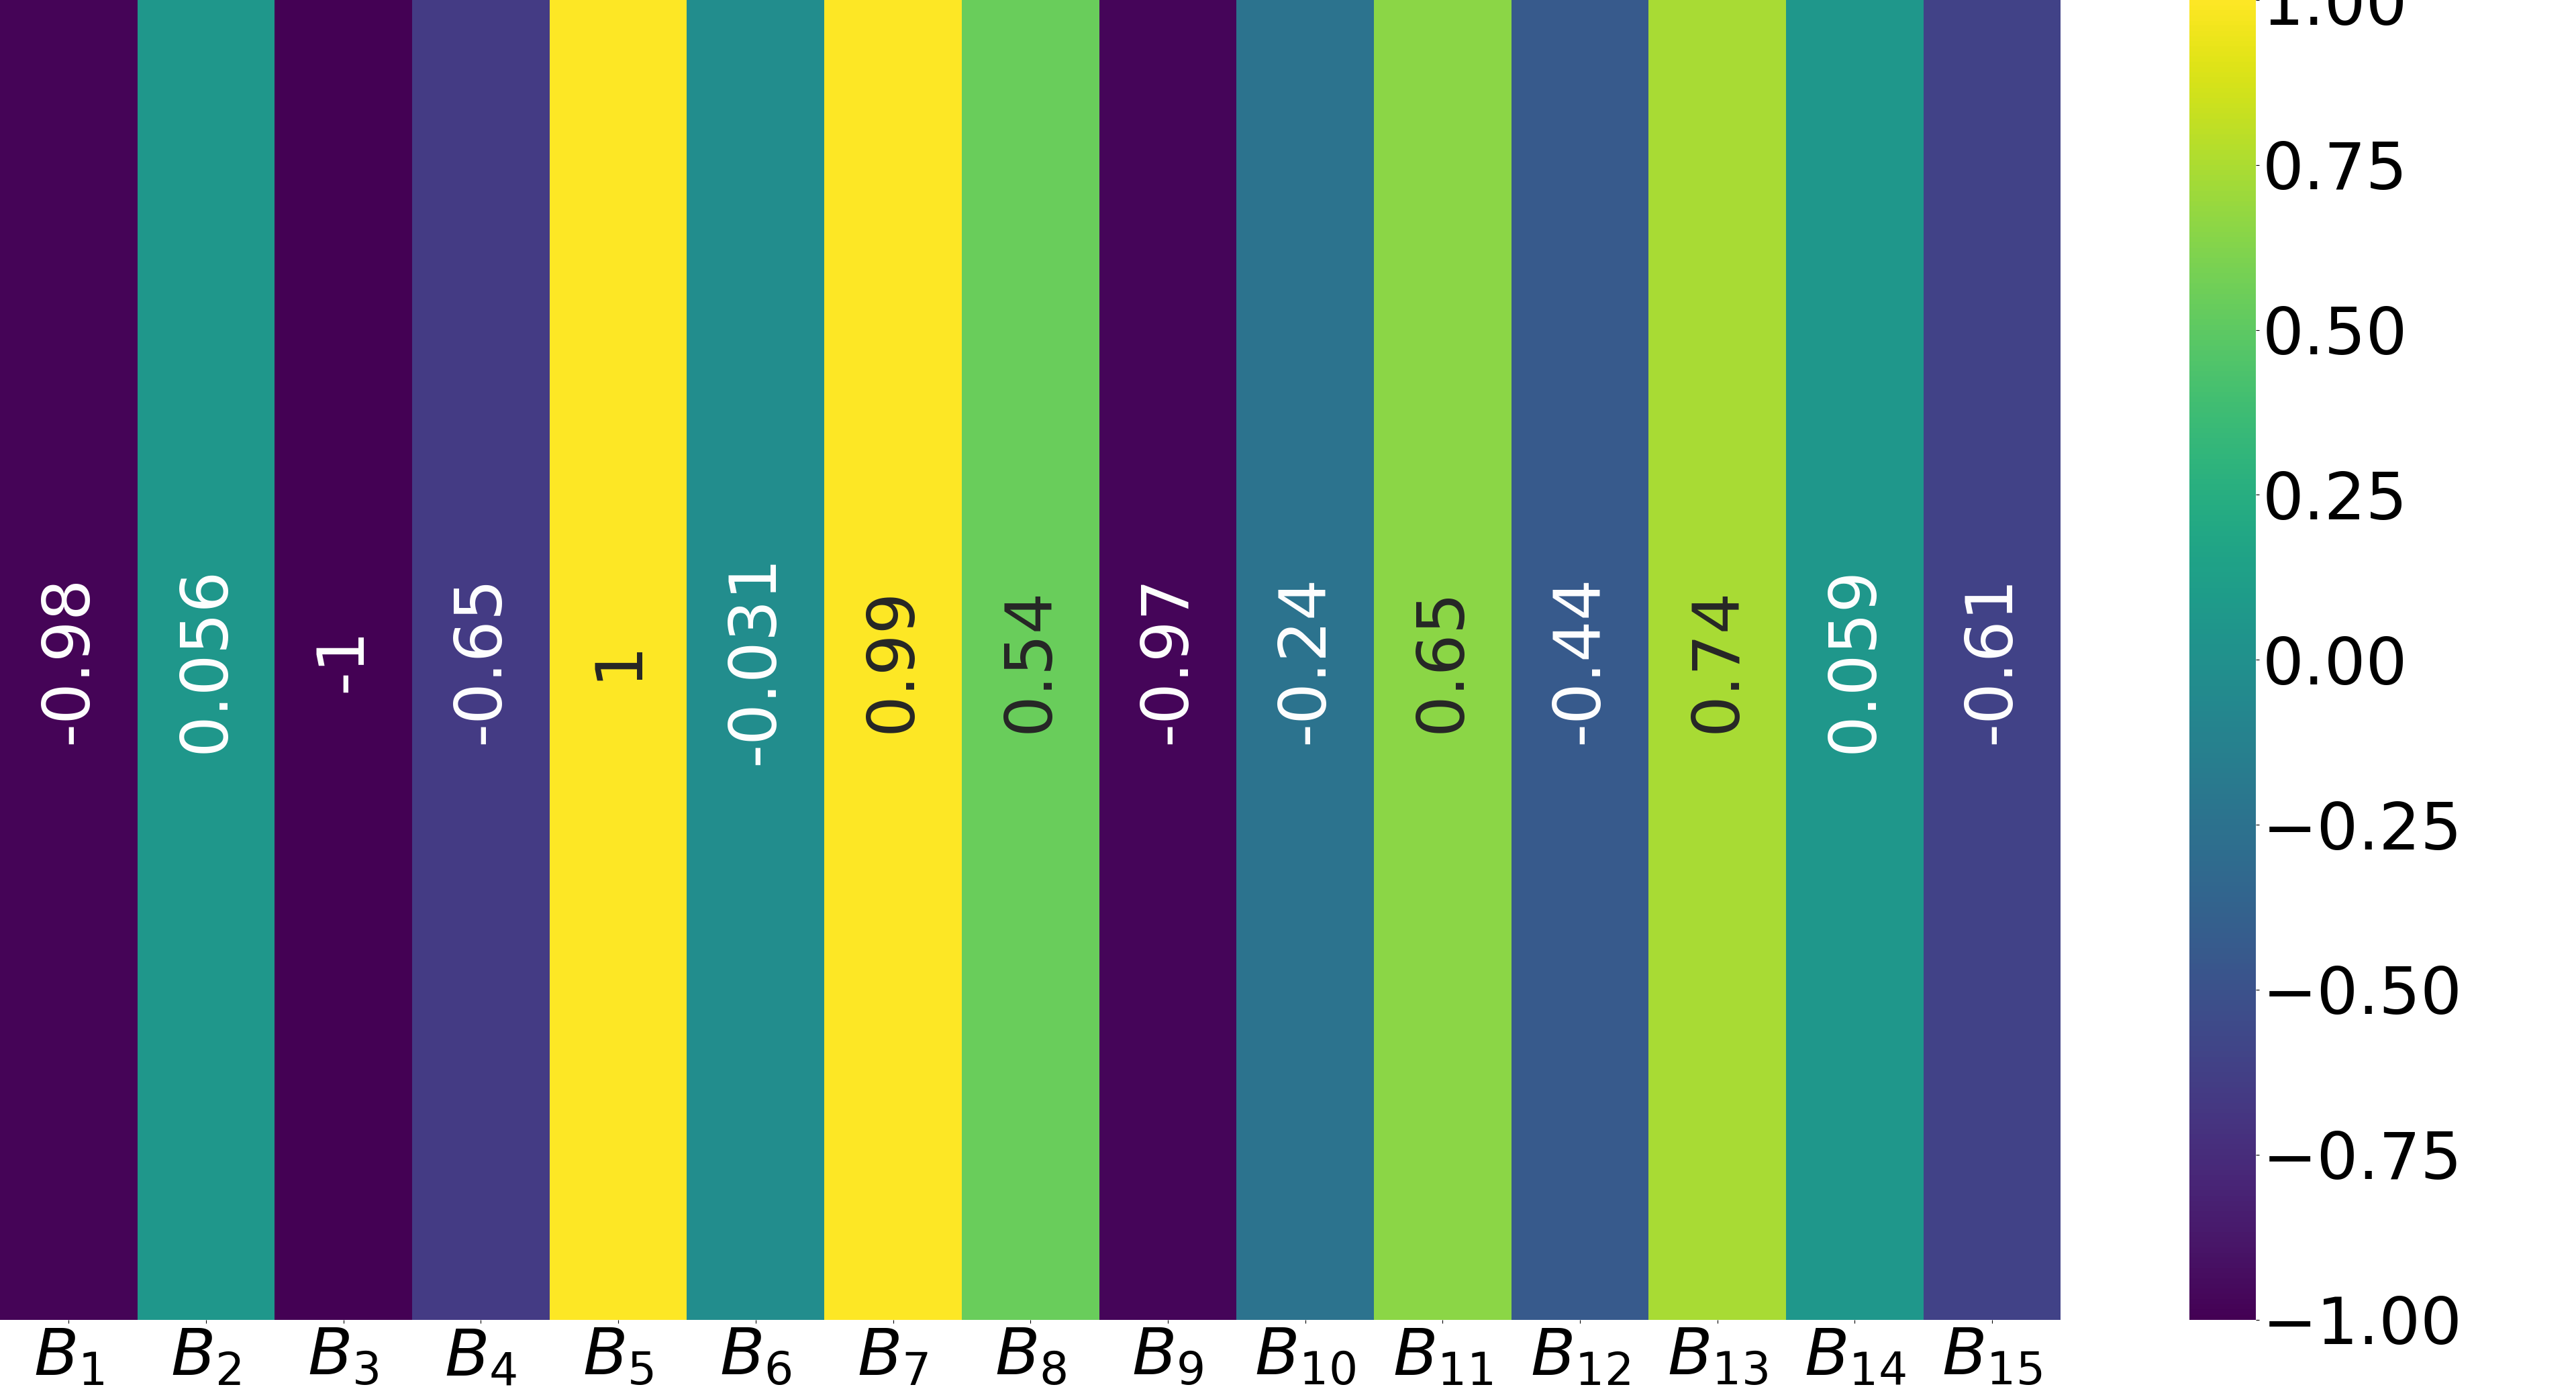
\includegraphics[width=\linewidth]{img/qlp_corr/Bn_coil3.png}
		\subcaption{Correlation with coil $3$}
	\end{subfigure}
	\caption{Correlation between the harmonics of the \bn\ attribute and the labels for \qlp.}
	\label{fig:bn-lcorr-qlp}
\end{figure}

\Cref{fig:bn-lcorr-qlp} highlights the correlation between \bn\ harmonics and the label associated
to each coil (as described in \Cref{chp:problem}). The attribute, similarly to \an, sees a pattern
of strong correlations between its odd-numbered harmonics and coils $1$ and $3$. Since the pattern
of sub-figures (b) and (d) is very similar to the one shown in sub-figures (a) and (c) of
\Cref{fig:an-lcorr-qlp}, we imagined that a plausible dataset composition would have followed rules
similar to the ones identified for \an.

In \Cref{fig:bn-coilq-dist} we visualized the samples in \bn\ after a round of \pca. Independently
of the sub-figure we consider it's clear that the level of homogeneity of the samples belonging to
the central cluster is very high. This was a phenomenon that we had already identified in
\Cref{sec:bn}, and, while this alone cannot induce us to think that the performance of models based
on \bn\ is going to be bad, we are drawn to consider the possibility that \bn\ might not be a good
enough attribute if taken on its own.
\begin{figure}[!ht]
	% Font size = 40
	\centering
	\begin{subfigure}{0.6\linewidth}
		\centering
		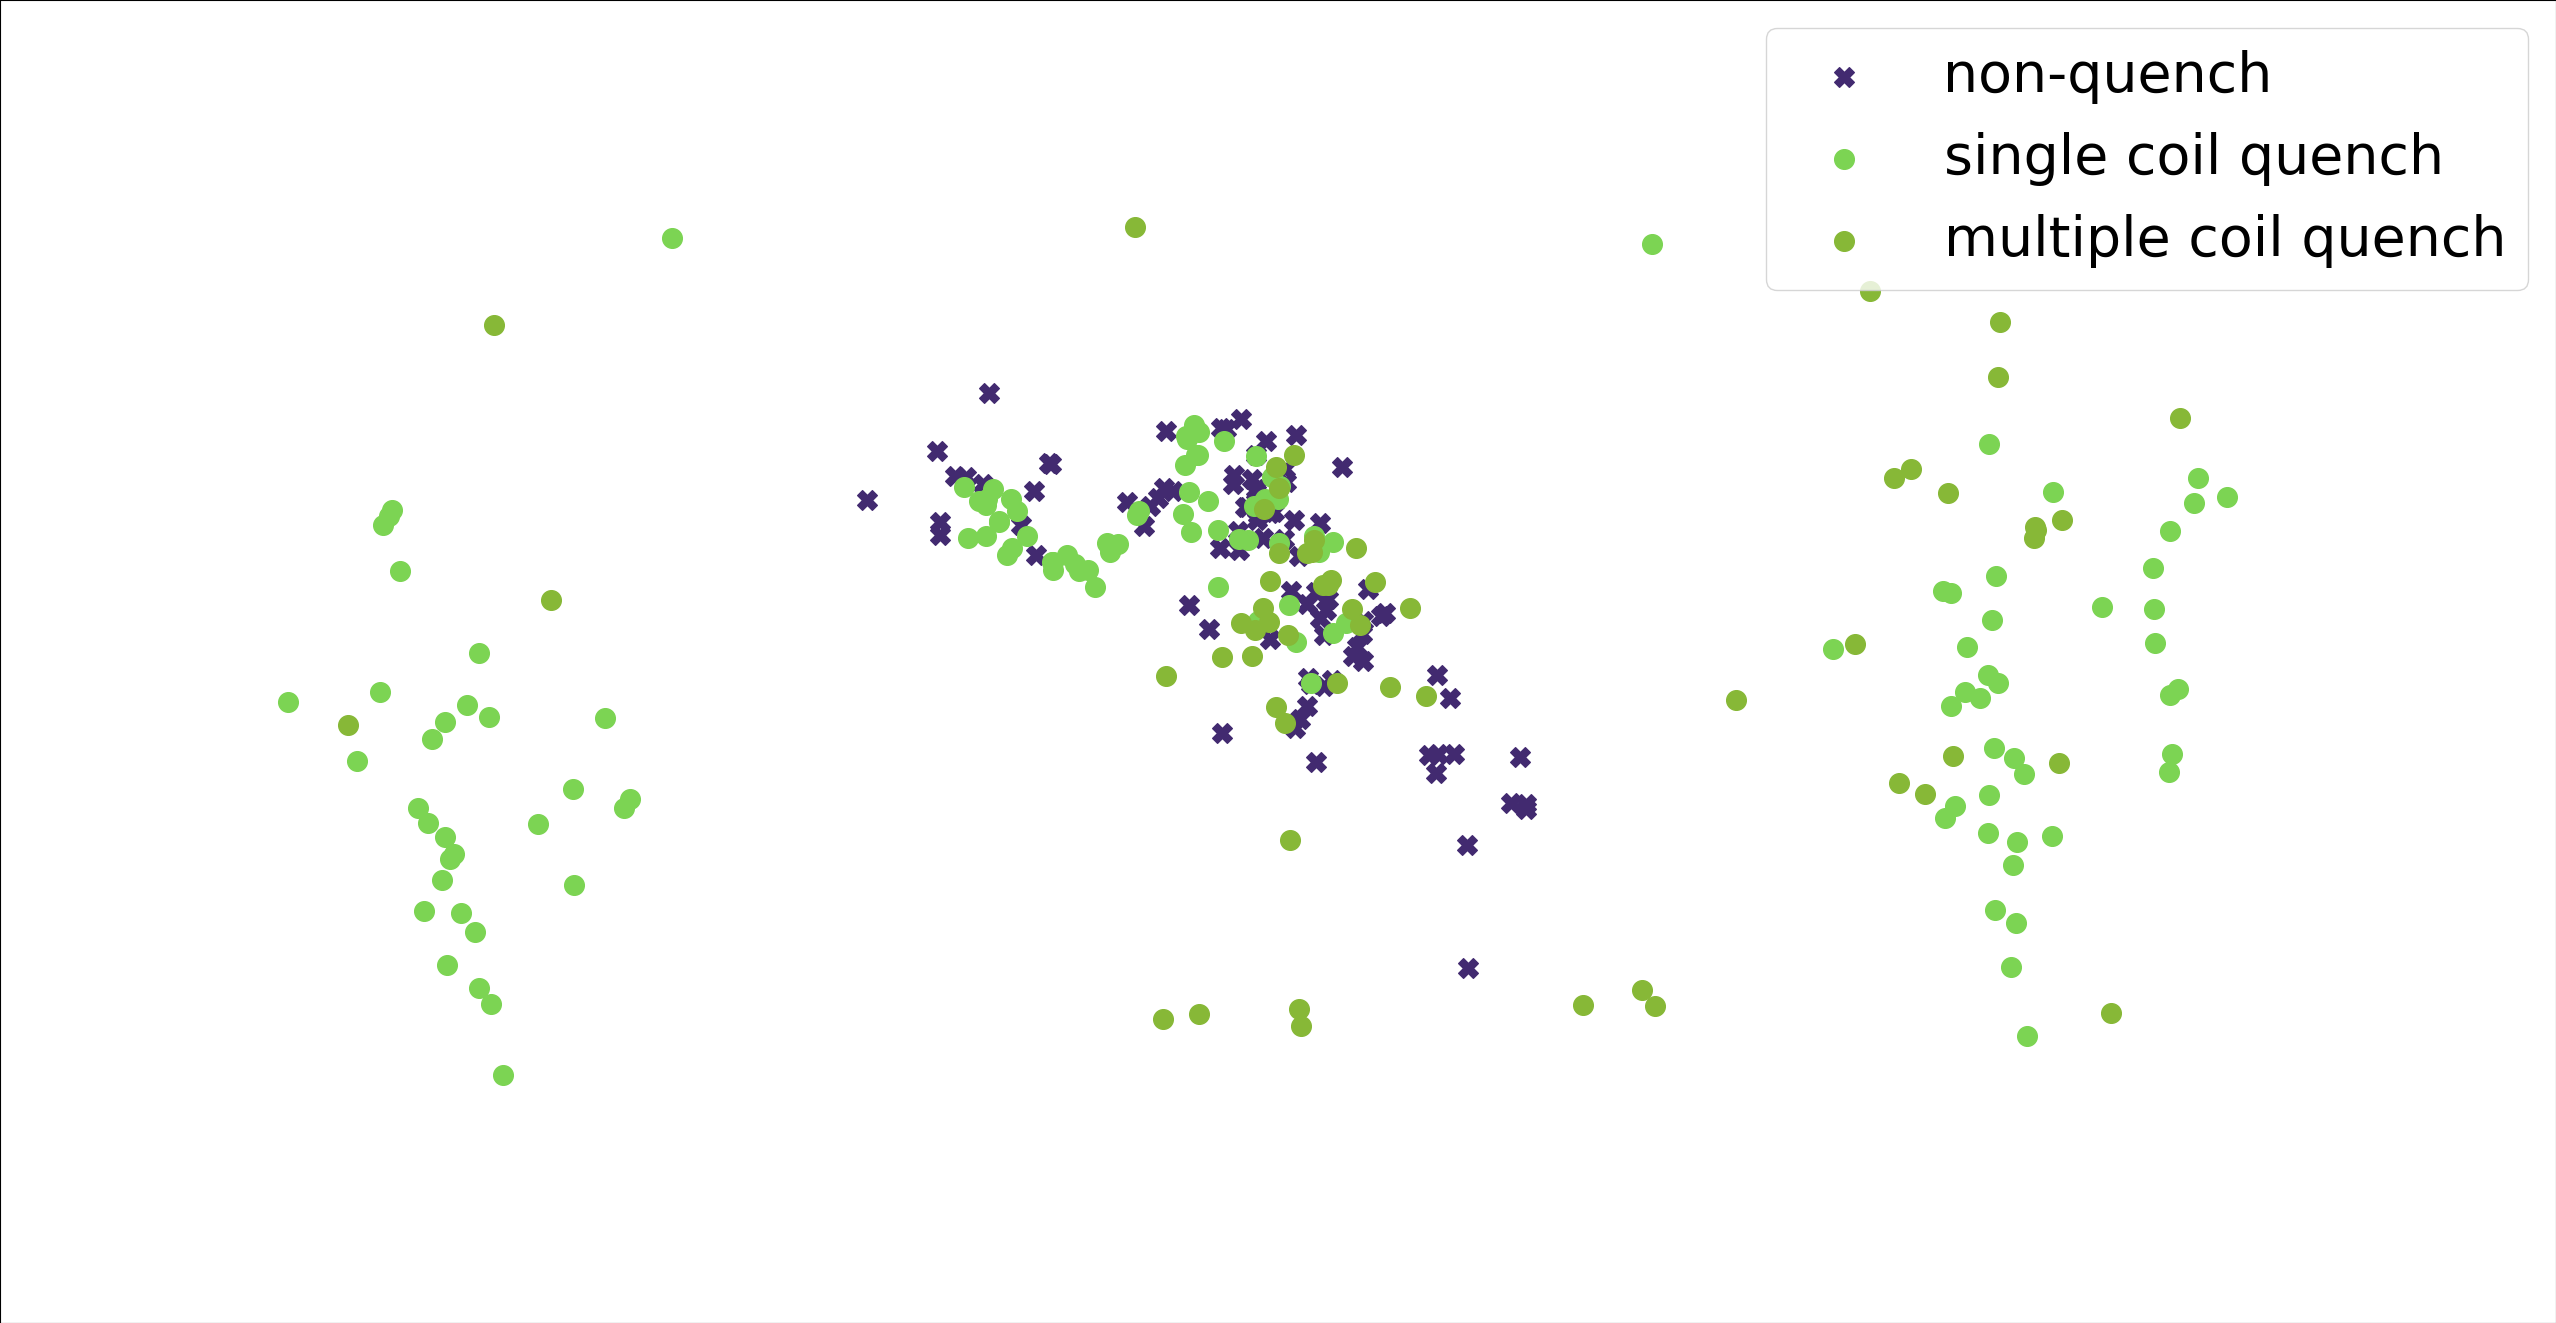
\includegraphics[width=\linewidth]{img/quench_dist_qlp/single_vs_multiple_Bn.png}
		\subcaption{}
	\end{subfigure}
	\begin{subfigure}{0.6\linewidth}
		\centering
		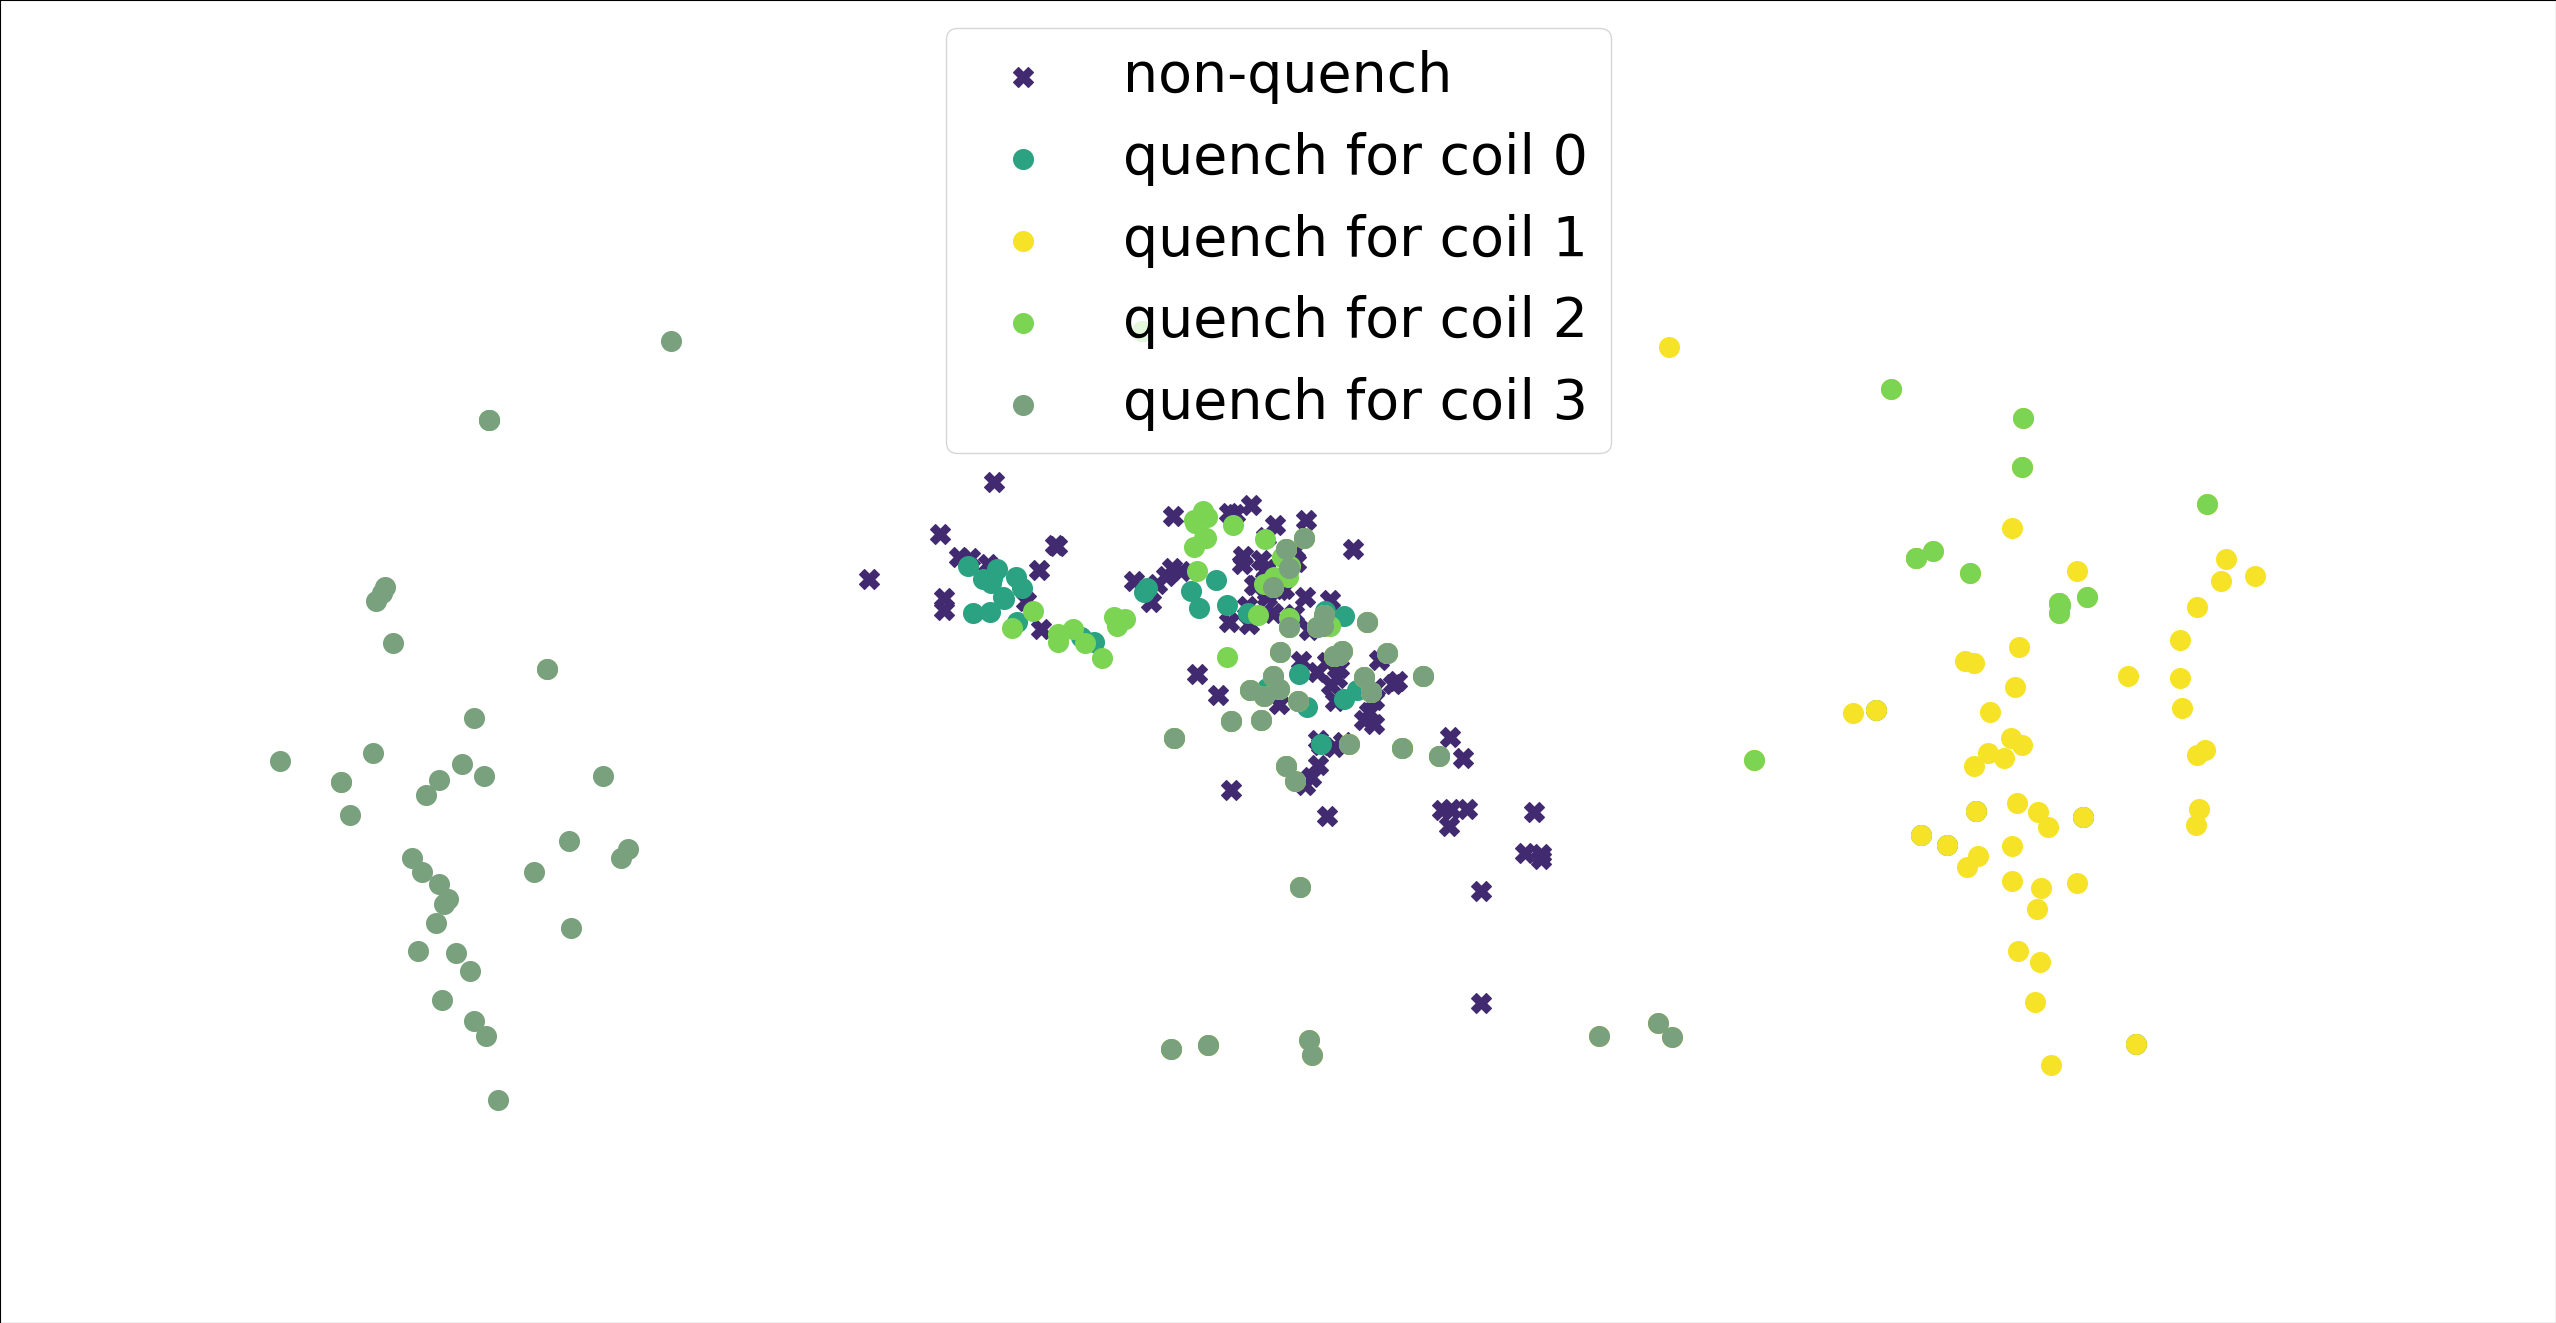
\includegraphics[width=\linewidth]{img/quench_dist_qlp_bn.png}
		\subcaption{}
	\end{subfigure}
	\caption{Visualization of the \bn\ attribute, the data was plotted after a run of \pca\
		dimensionality reduction. Sub-figure (a) highlights the samples based on how many quenches
		are associated to the specific sample $\{0, 1, \text{many}\}$. Sub-figure (b) highlights the
		samples based on the specific coil quenched $\{\text{None}, 0, 1, 2, 3\}$.}
	\label{fig:bn-coilq-dist}
\end{figure}

\subsubsection{\cnmod}
As we said in \Cref{chp:problem}, \cnmod\ was expected to be very informative for \qrp, but not for
\qlp. Interestingly, though, the correlation between the harmonics for the attribute and the labels
associated to each coil, shown in \Cref{fig:cnmod-lcorr-qlp}, seems to be telling a different story.
If we consider coils $0$ and $3$, we can see a very strong correlation between the harmonics and the
label, it's also worth noting that, in sub-figures (a) through (d), \cnmod[2]\ seems to be extremely
important to explain the value associated with the labels.
\begin{figure}[!ht]
	% Font size = 70
	\centering
	\begin{subfigure}{0.49\linewidth}
		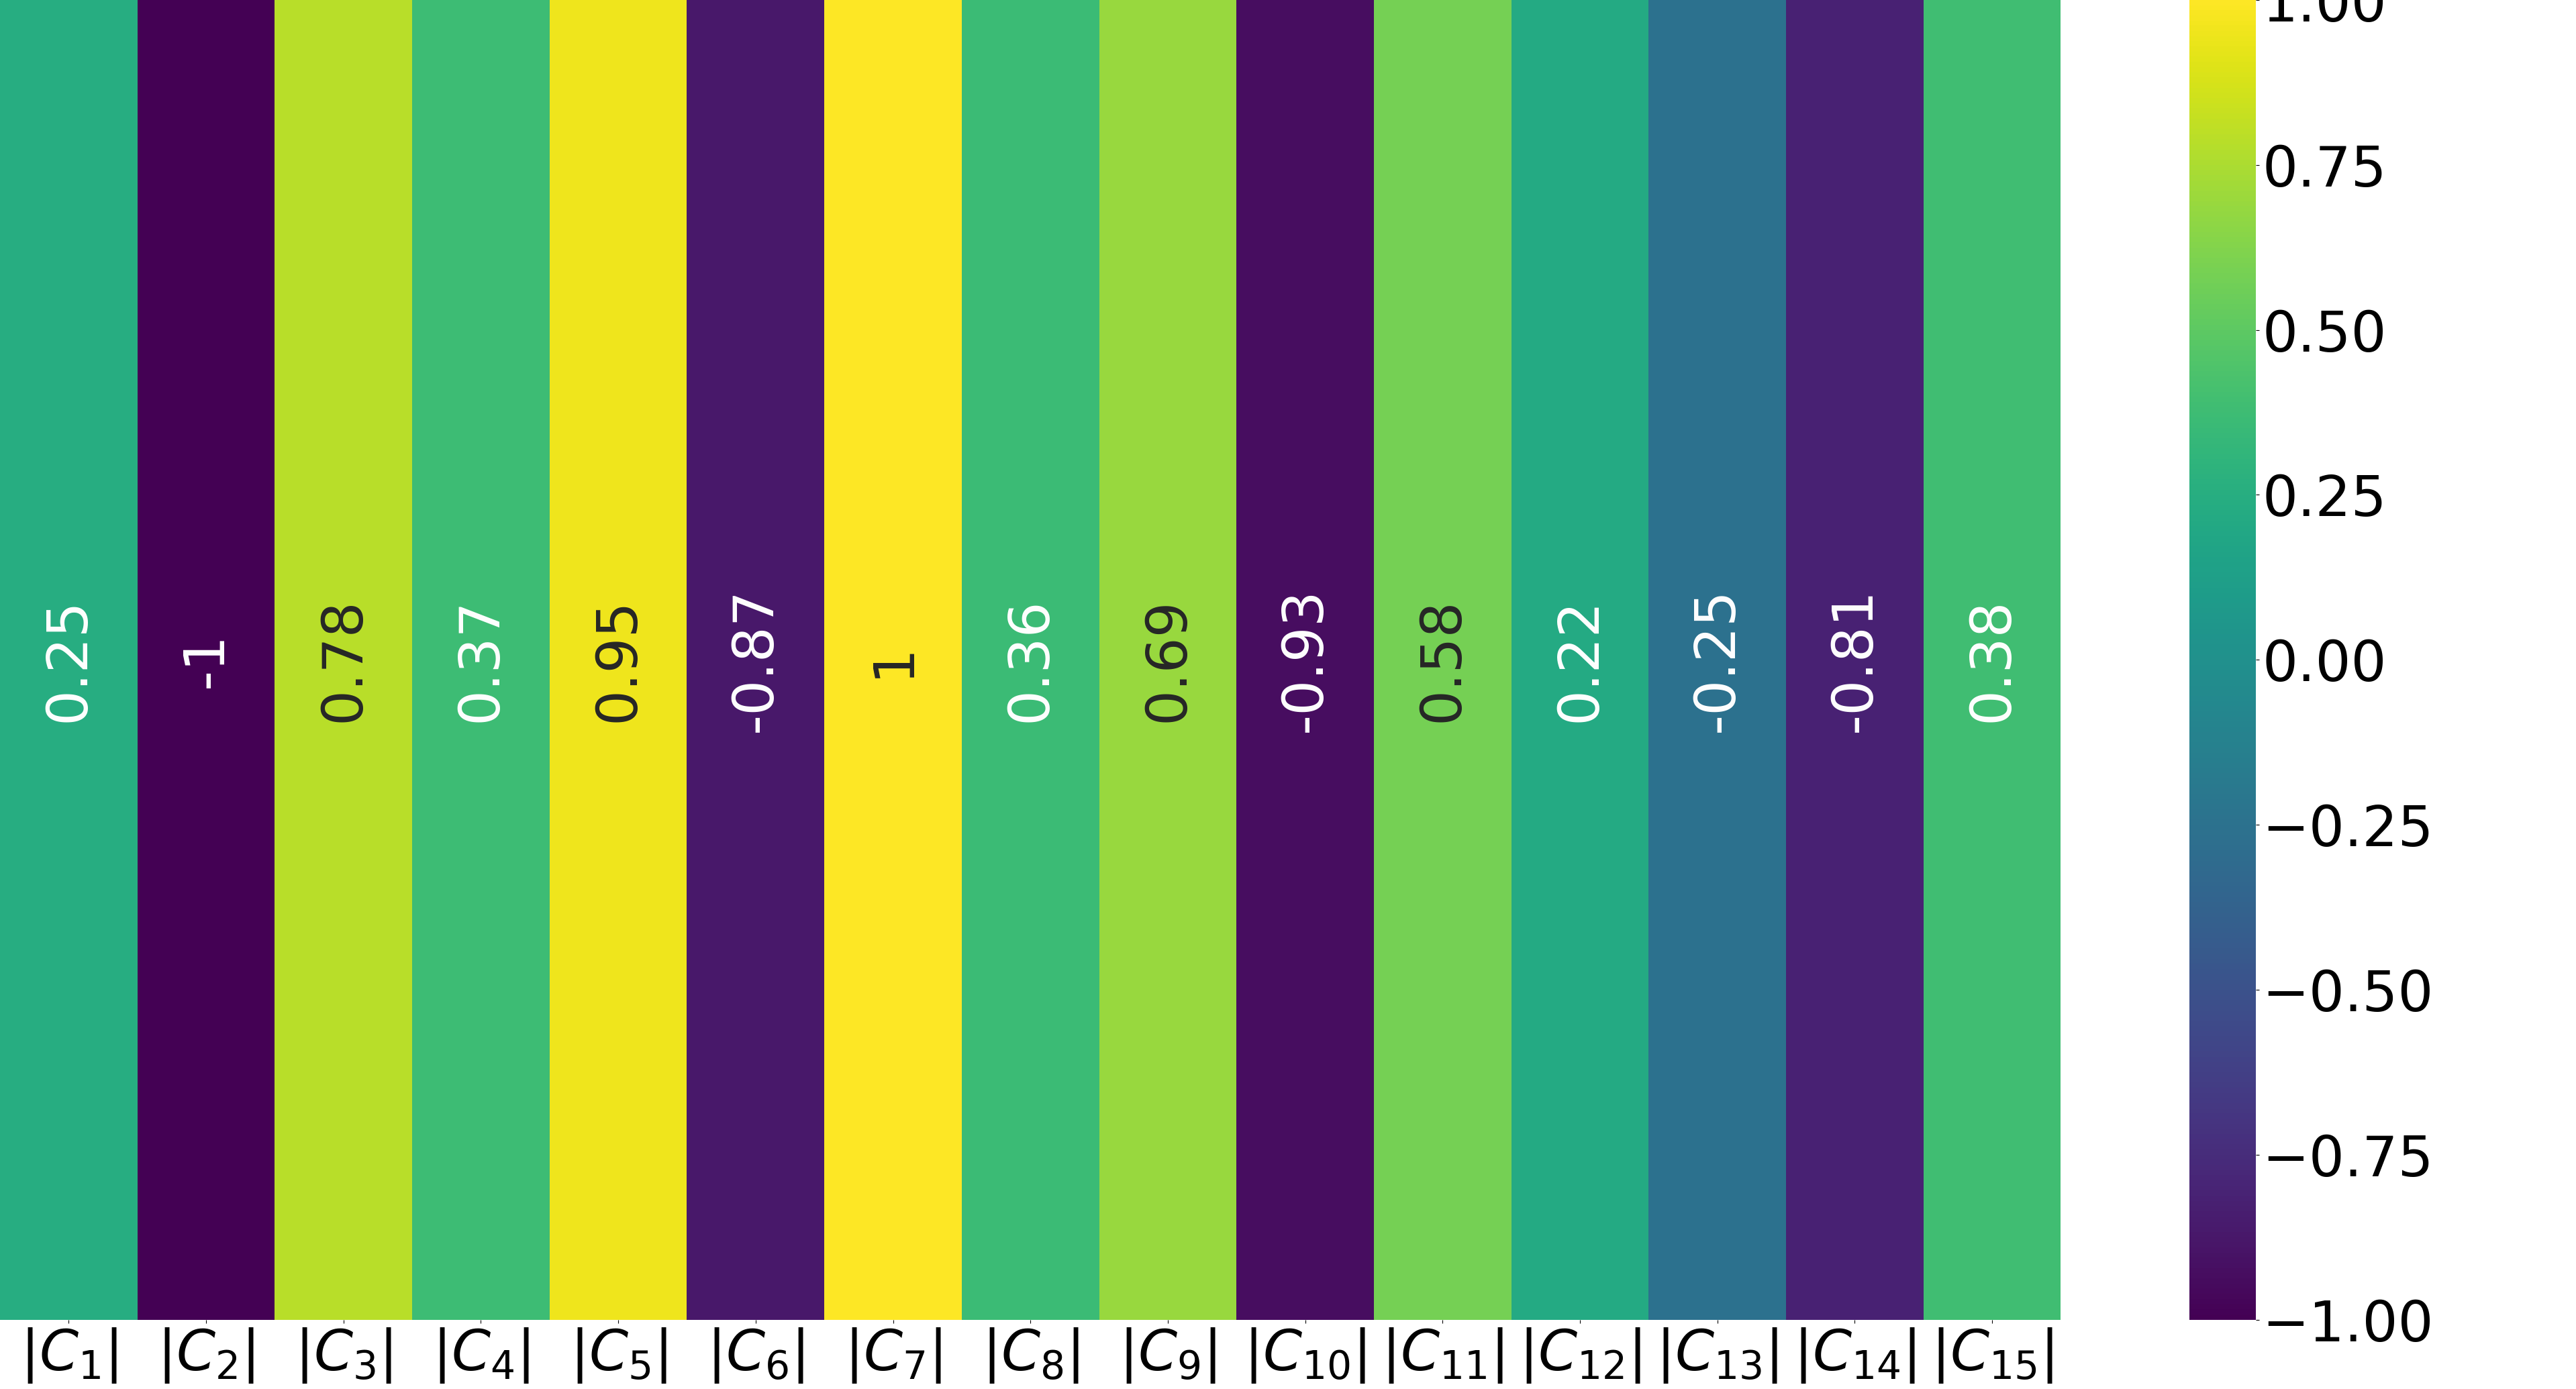
\includegraphics[width=\linewidth]{img/qlp_corr/Cnmod_coil0.png}
		\subcaption{Correlation with coil $0$}
	\end{subfigure}
	\begin{subfigure}{0.49\linewidth}
		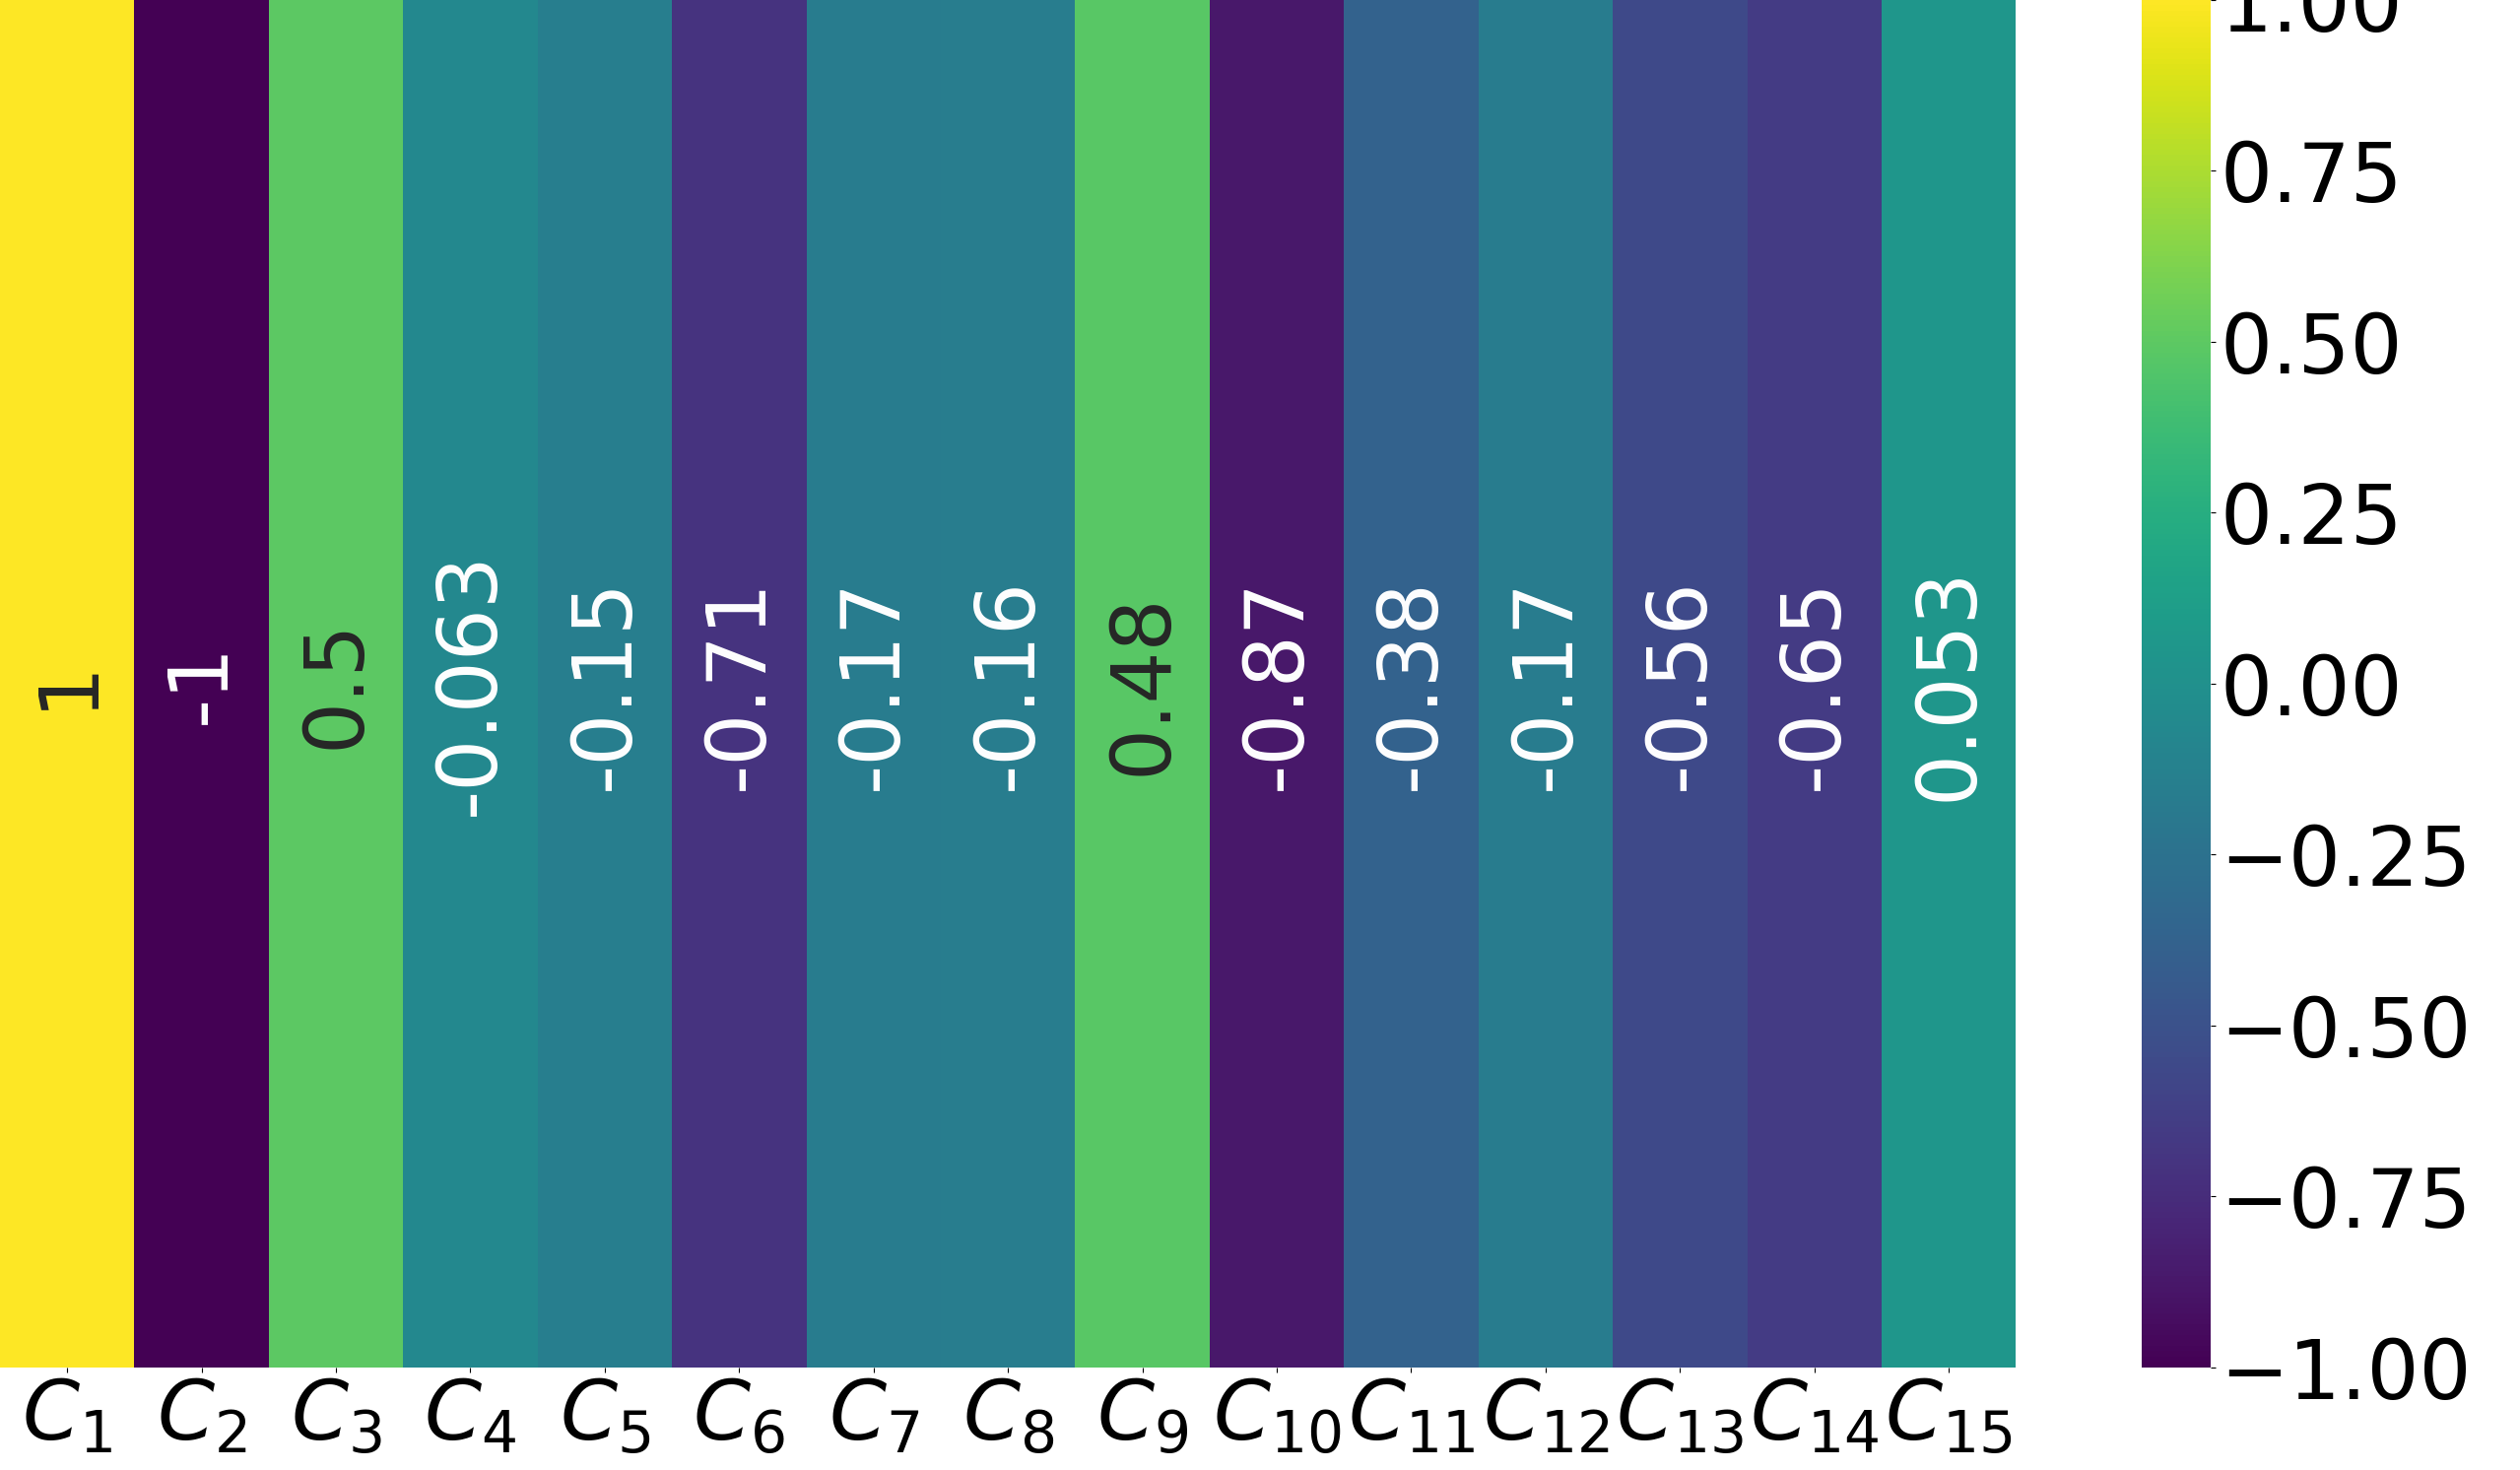
\includegraphics[width=\linewidth]{img/qlp_corr/Cnmod_coil1.png}
		\subcaption{Correlation with coil $1$}
	\end{subfigure}
	\begin{subfigure}{0.49\linewidth}
		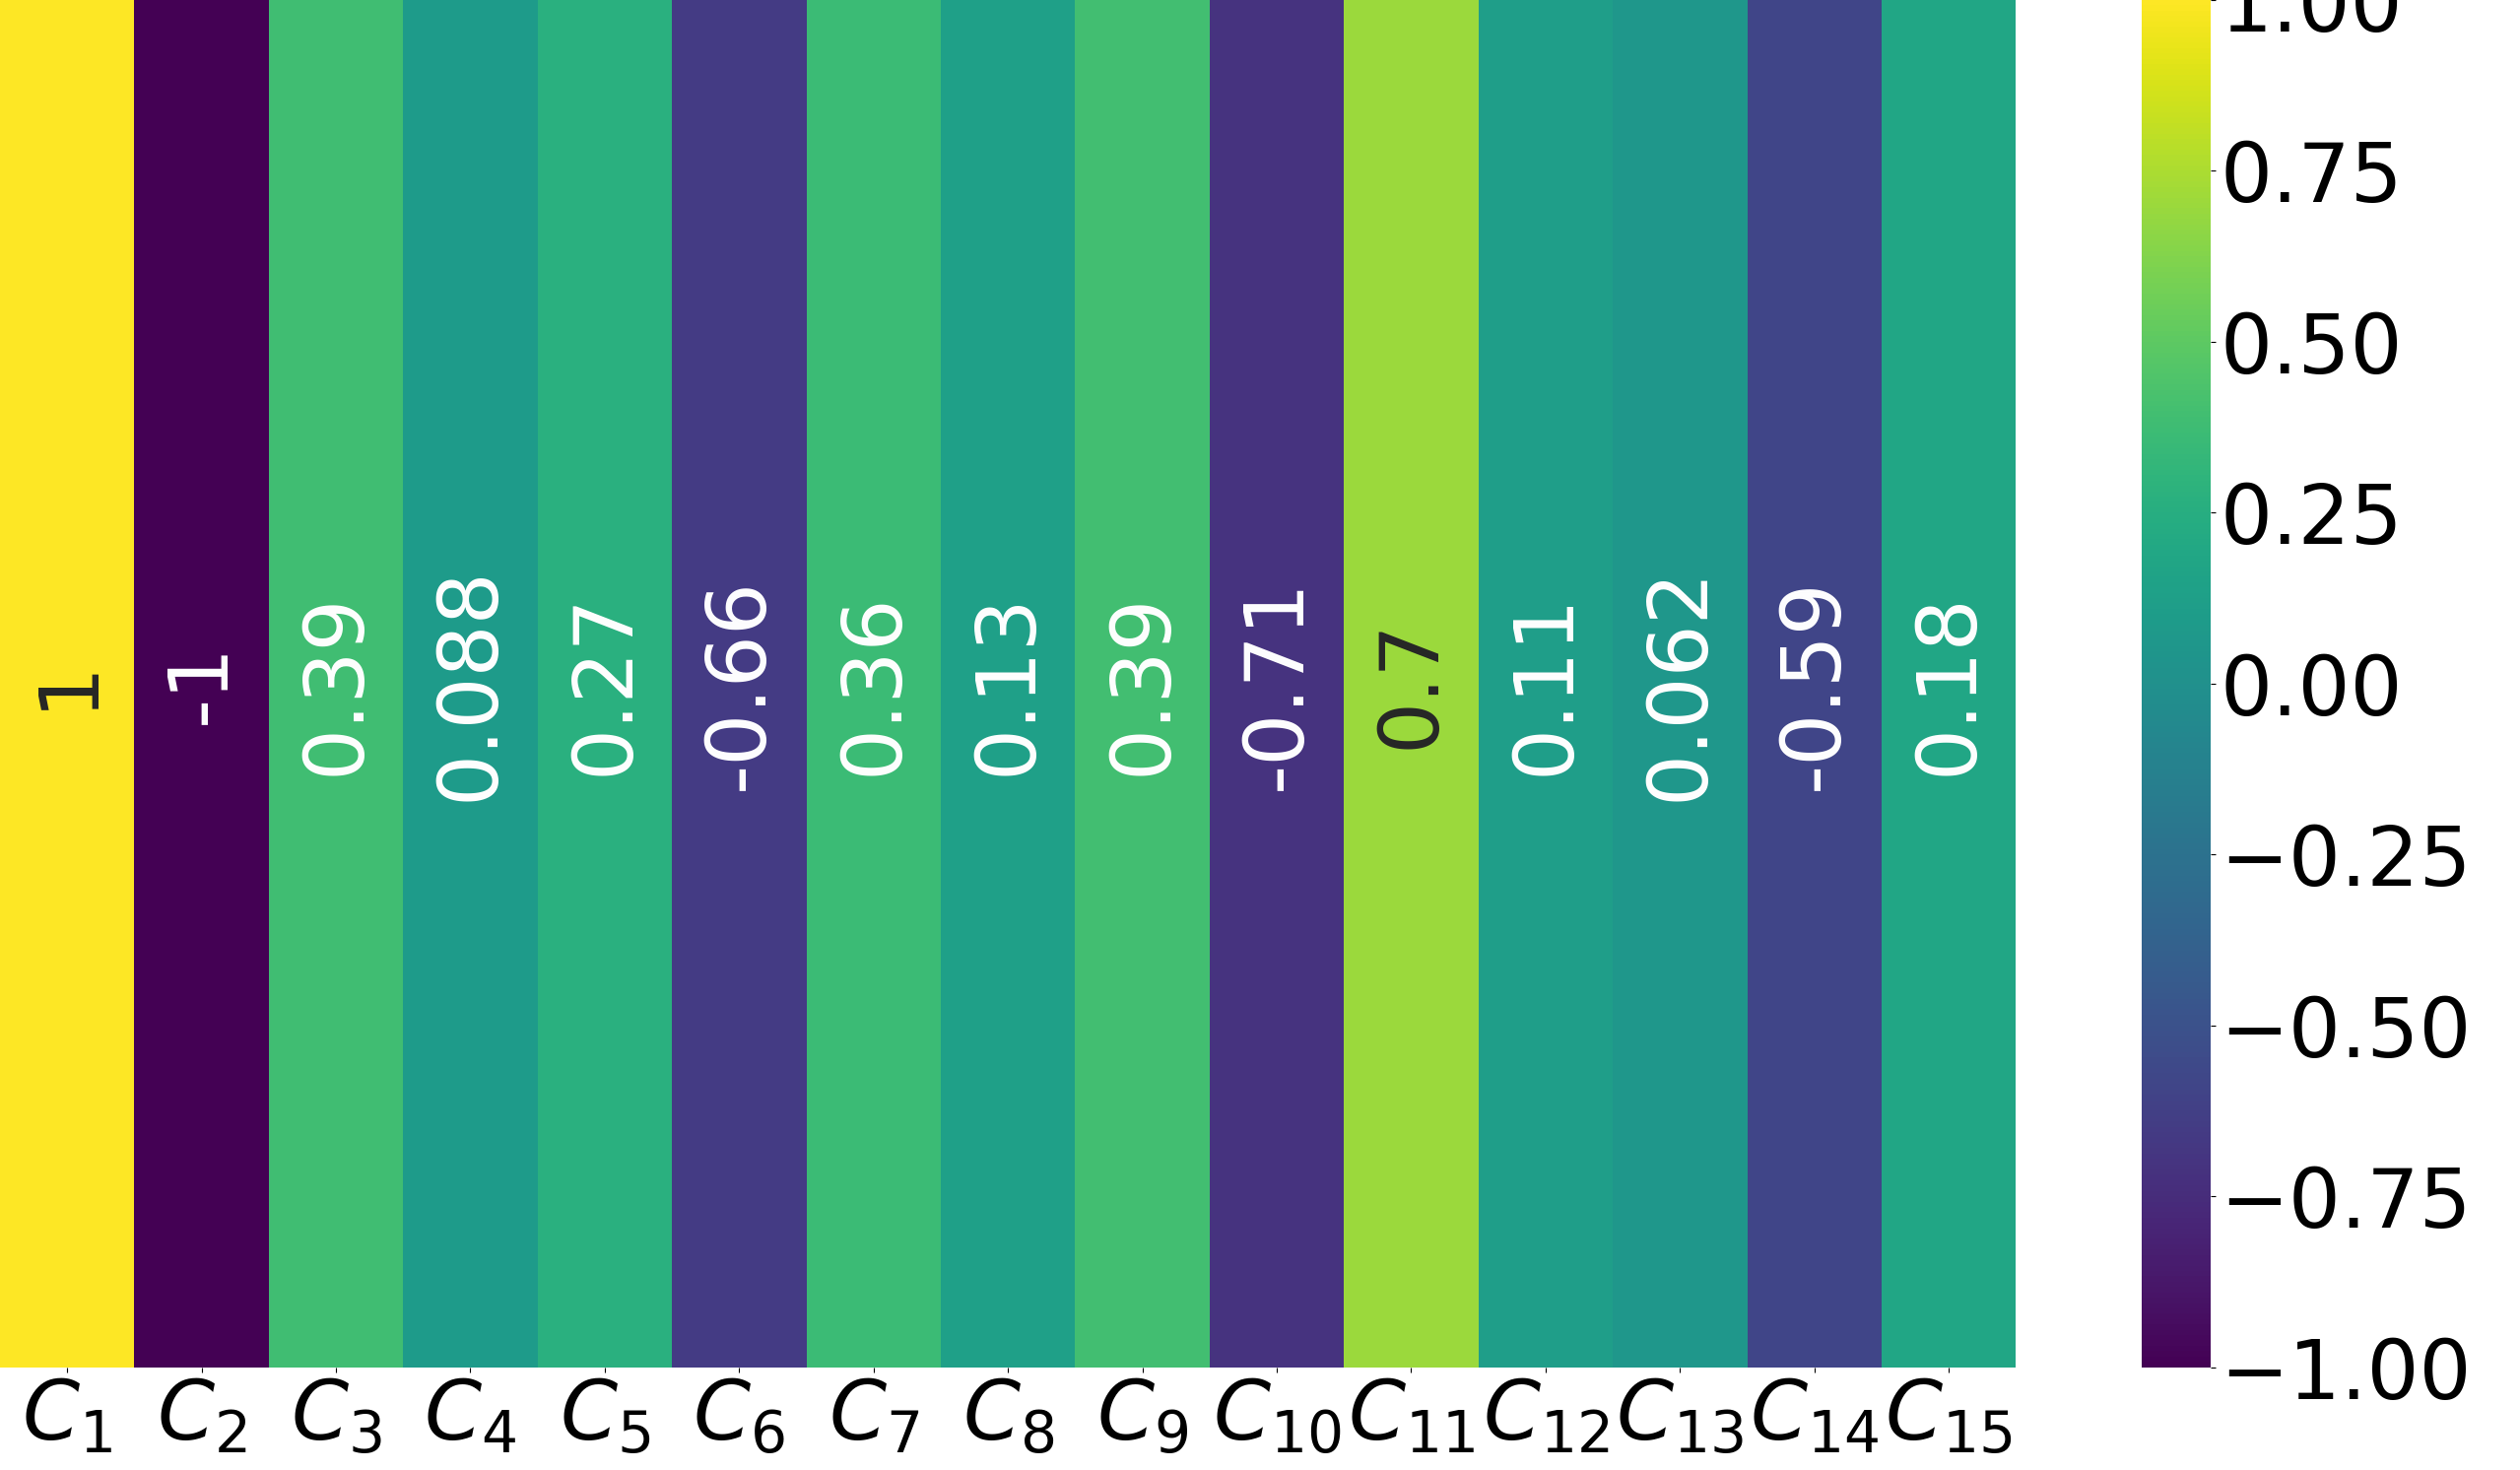
\includegraphics[width=\linewidth]{img/qlp_corr/Cnmod_coil2.png}
		\subcaption{Correlation with coil $2$}
	\end{subfigure}
	\begin{subfigure}{0.49\linewidth}
		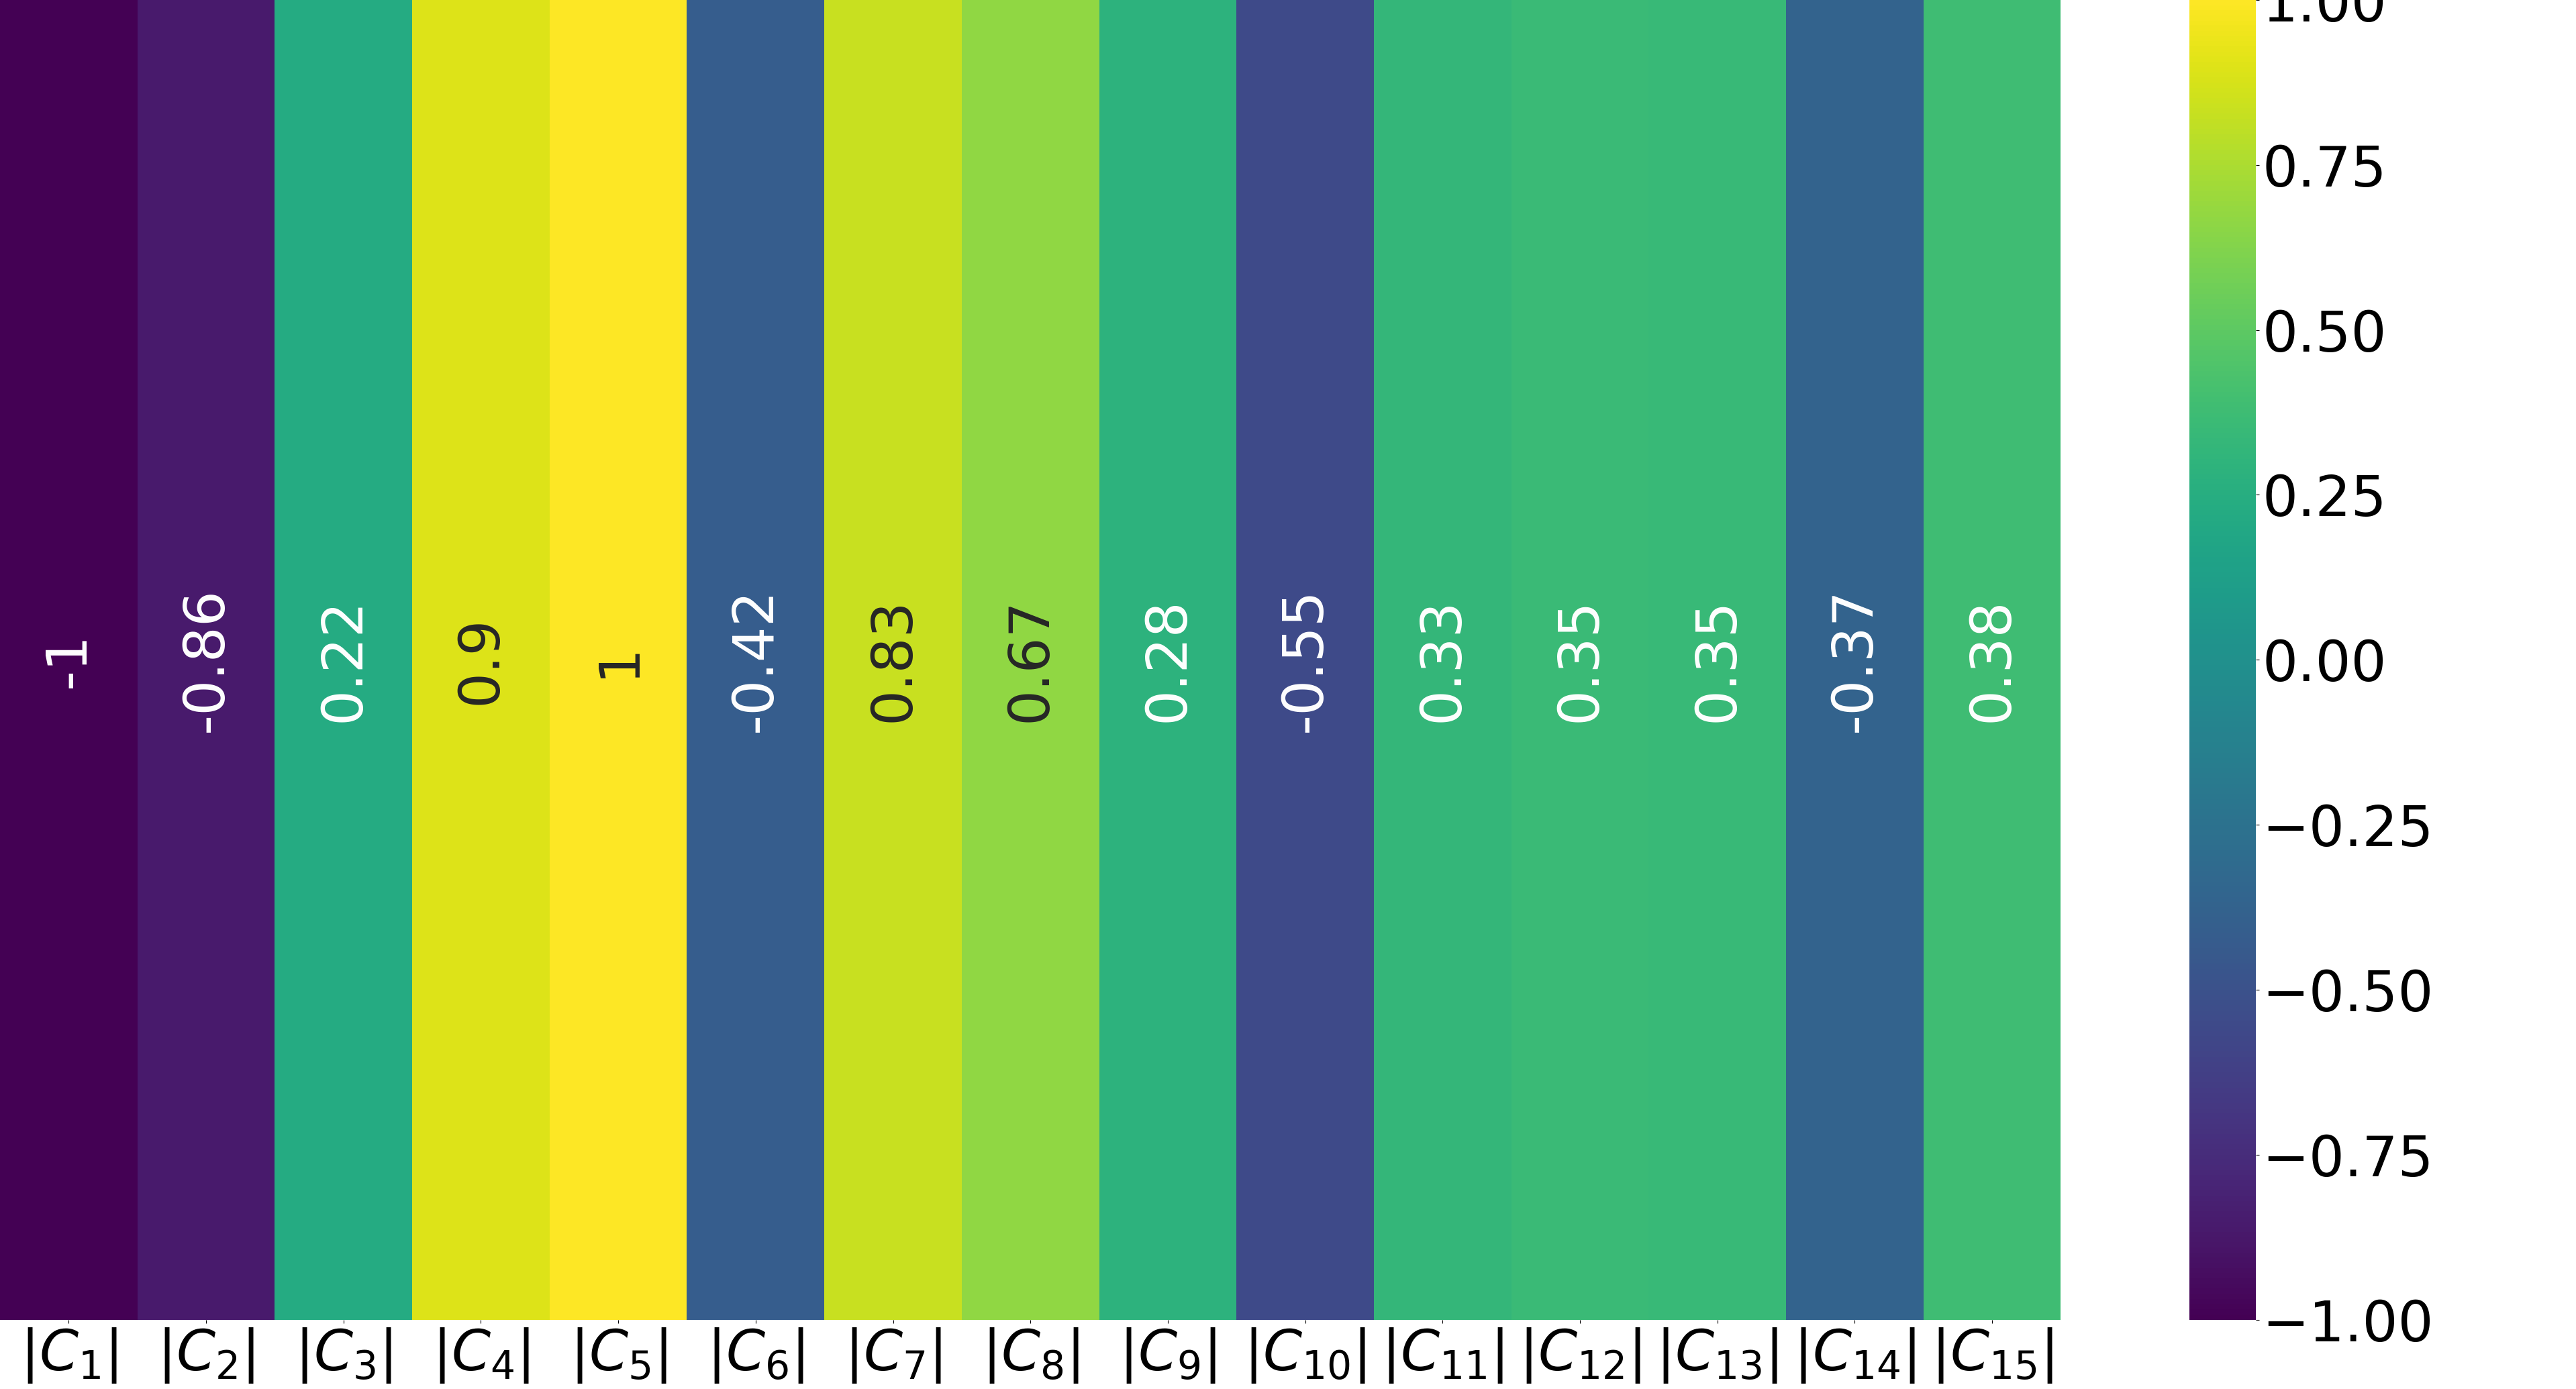
\includegraphics[width=\linewidth]{img/qlp_corr/Cnmod_coil3.png}
		\subcaption{Correlation with coil $3$}
	\end{subfigure}
	\caption{Correlation between the harmonics of the \cnmod\ attribute and the labels for \qlp.}
	\label{fig:cnmod-lcorr-qlp}
\end{figure}

If we look back at the correlation matrix computed for \cnmod\ during the preprocessing for \qrp\
(see \Cref{fig:cnmod-corr} and \Cref{sec:cnmod}) a sub-view of \cnmod\ could be built as follows.
\begin{itemize}
	\item For coil $0$, \cnmod[2] and a high-order candidate. While this would
		technically maximize the total correlation with the label, we have seen in \qrp\
		that choosing \cnmod[2]\ was a choice that didn't pay. That is why we might select
		\cnmod[3] or \cnmod[6] in the end, accompanied by another high order harmonic like
		\cnmod[9] or \cnmod[11].
	\item For coil $3$, we could be taking harmonic \cnmod[1] and then using one or more from
	      \{\cnmod[4], \cnmod[5], \cnmod[6], \cnmod[7], \cnmod[8]\}; finally, if it leads to
	      better performance, we could also add another high-order harmonic like \cnmod[10].
\end{itemize}
\begin{figure}[!ht]
	% Font size = 40
	\centering
	\begin{subfigure}{0.6\linewidth}
		\centering
		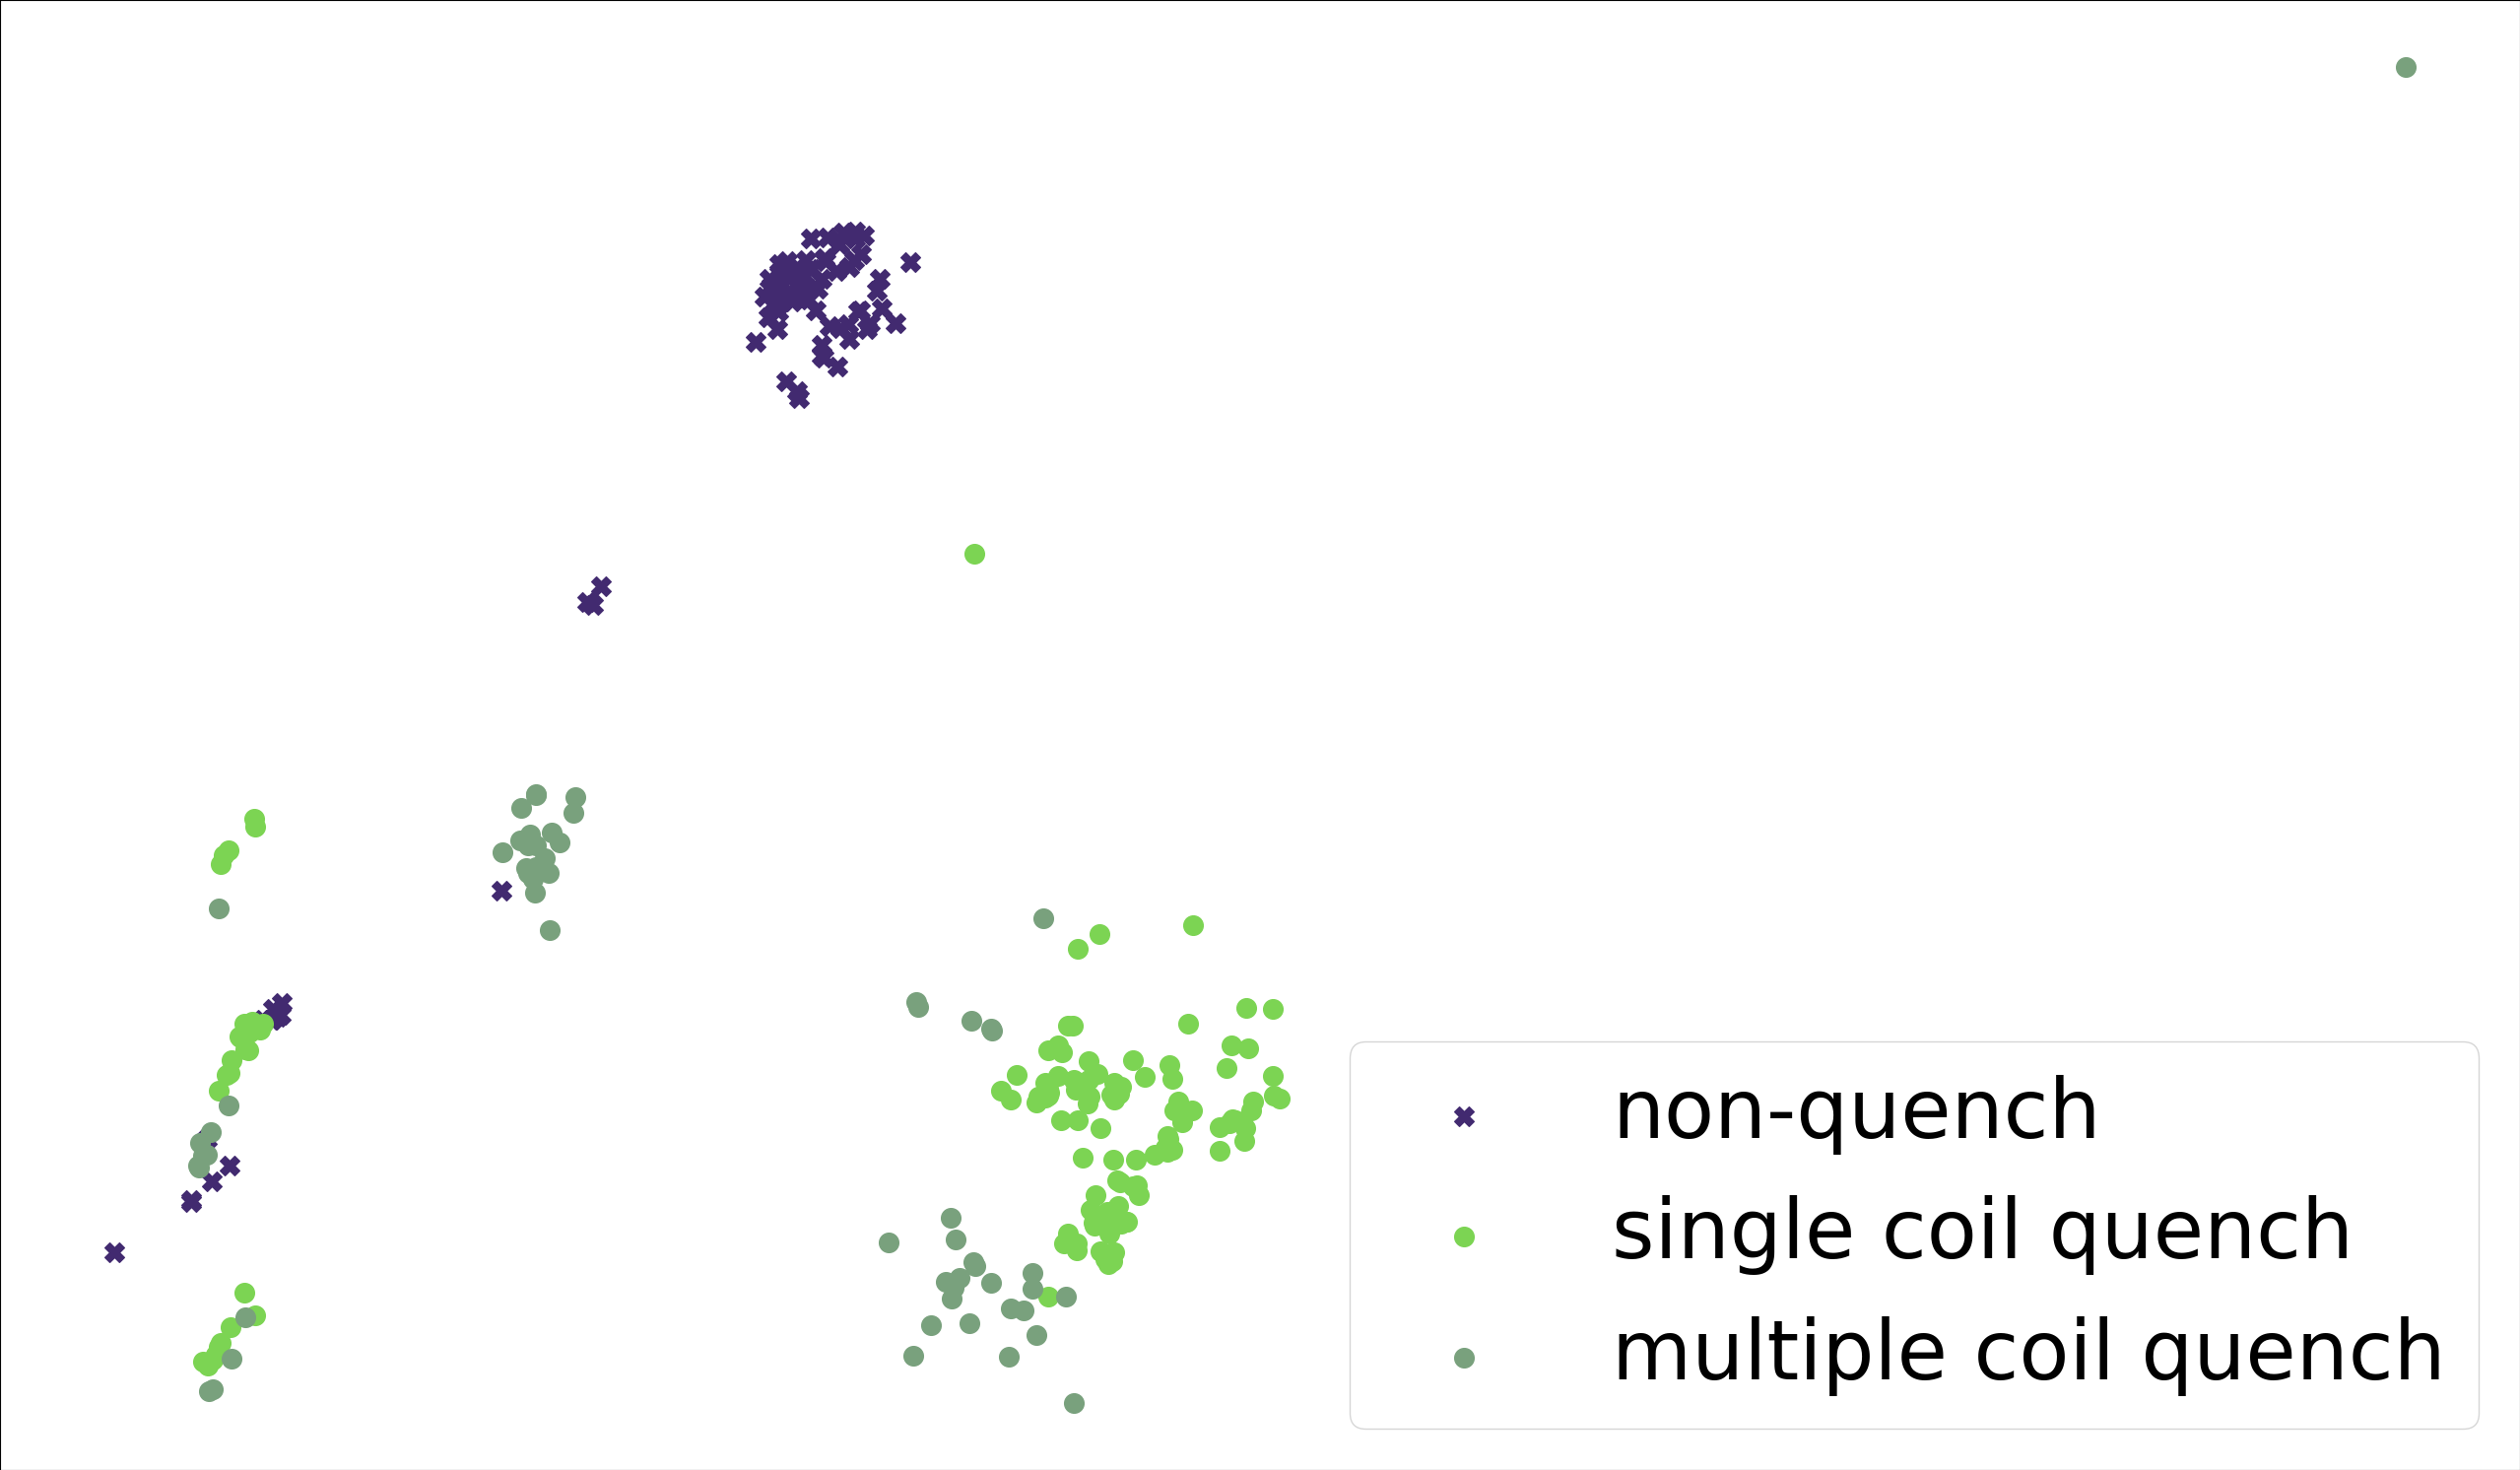
\includegraphics[width=\linewidth]{img/quench_dist_qlp/single_vs_multiple_Cnmod.png}
		\subcaption{}
	\end{subfigure}
	\begin{subfigure}{0.6\linewidth}
		\centering
		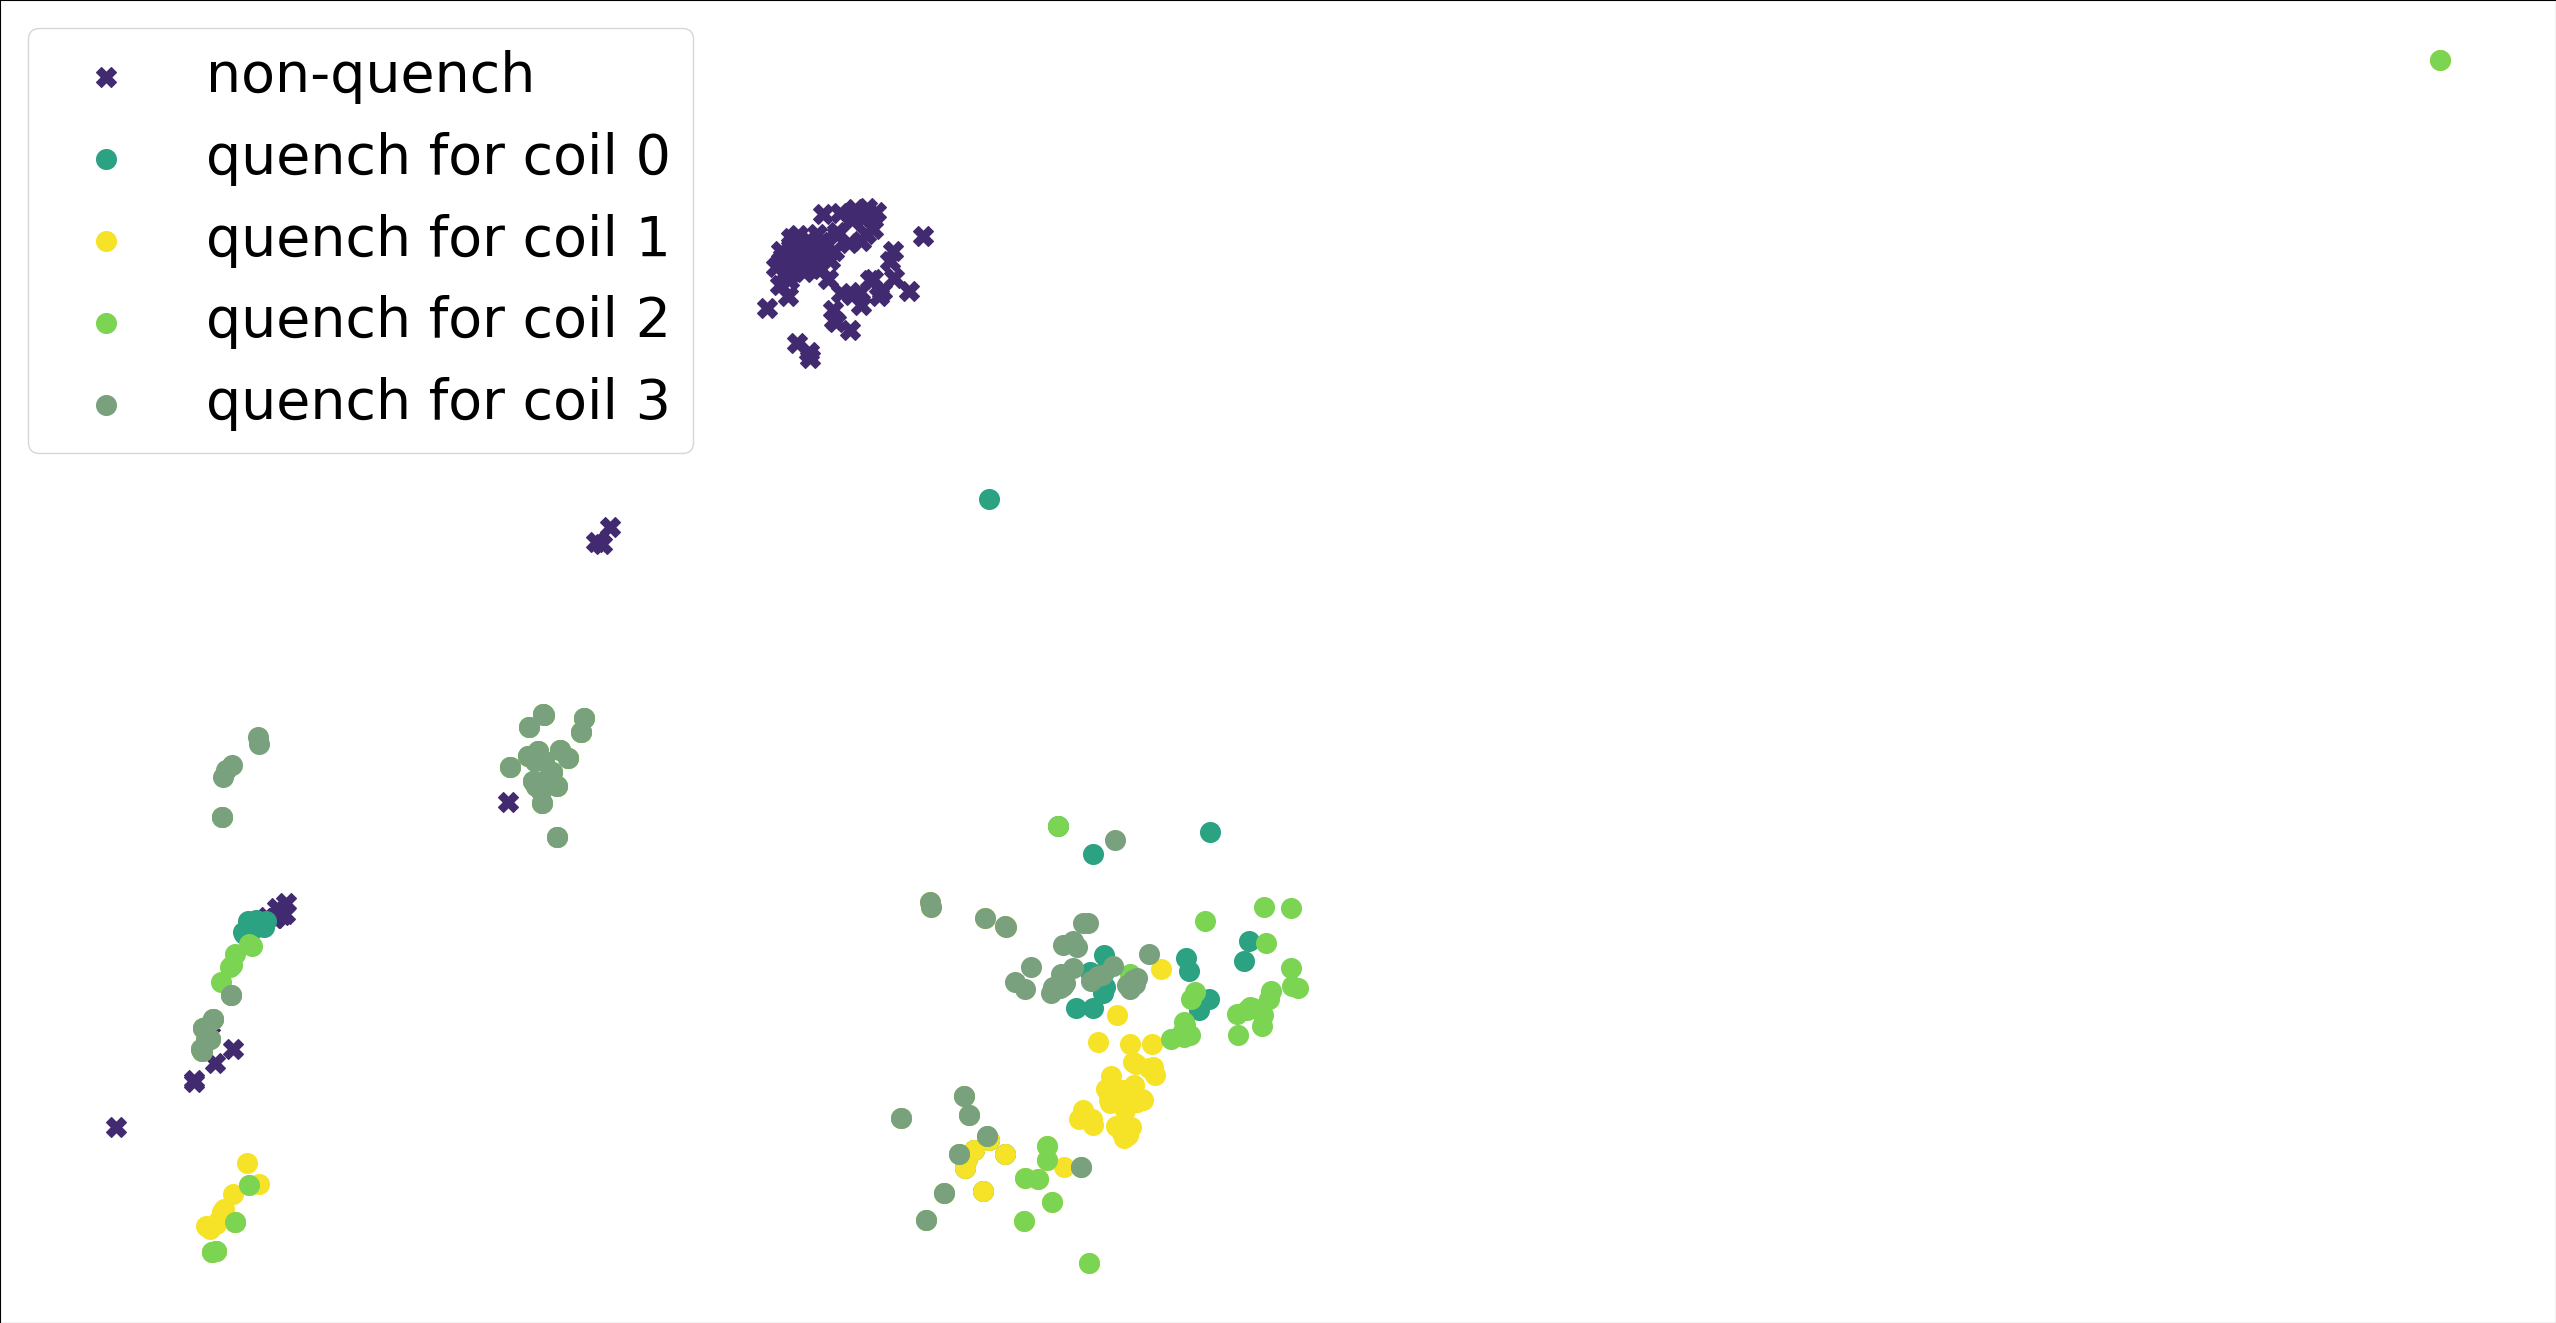
\includegraphics[width=\linewidth]{img/quench_dist_qlp_cnmod.png}
		\subcaption{}
	\end{subfigure}
	\caption{Visualization of the \cnmod\ attribute, the data was plotted after a run of \pca\
		dimensionality reduction. Sub-figure (a) highlights the samples based on how many quenches
		are associated to the specific sample $\{0, 1, \text{many}\}$. Sub-figure (b) highlights the
		samples based on the specific coil quenched $\{\text{None}, 0, 1, 2, 3\}$.}
	\label{fig:cnmod-coilq-dist}
\end{figure}

As we did for \an\ and \bn, we visualized \cnmod\ after a round of \pca\ dimensionality reduction.
\Cref{fig:cnmod-coilq-dist} shows a similar situation to \an, if we consider the specific case of
sub-figure (a), while the clusters are not as clean cut as the alternative, there is much more
separation of the classes compared to \bn. As far as single coil quench is concerned (see sub-figure
(b)), there is clearly a high degree of homogeneity, especially in the cluster in the bottom right,
where we can see many points labelled differently but located very close together.

\subsubsection{\phin}
To close the section we are going to consider the \phin\ attribute. In \Cref{fig:phi-lcorr-qlp} we
plotted the cross-correlation between the harmonics and the labels. Due to how high the correlation
is between most harmonics and basically all the coils, we might be lead to think that this is the
best attribute available to us. This hypothesis is corroborated by the fact that, in the original
work~\cite{mariotto2022}, the identification of the quenched coil was done by computing the averaged
phase of the residual magnetic field. Since the harmonics are also very weakly correlated among themselves
(see \Cref{fig:phi-corr} and \Cref{sec:phi}), we just chose to not extract any features and use the
attribute as is.
\begin{figure}[!ht]
	% Font size = 70
	\centering
	\begin{subfigure}{0.49\linewidth}
		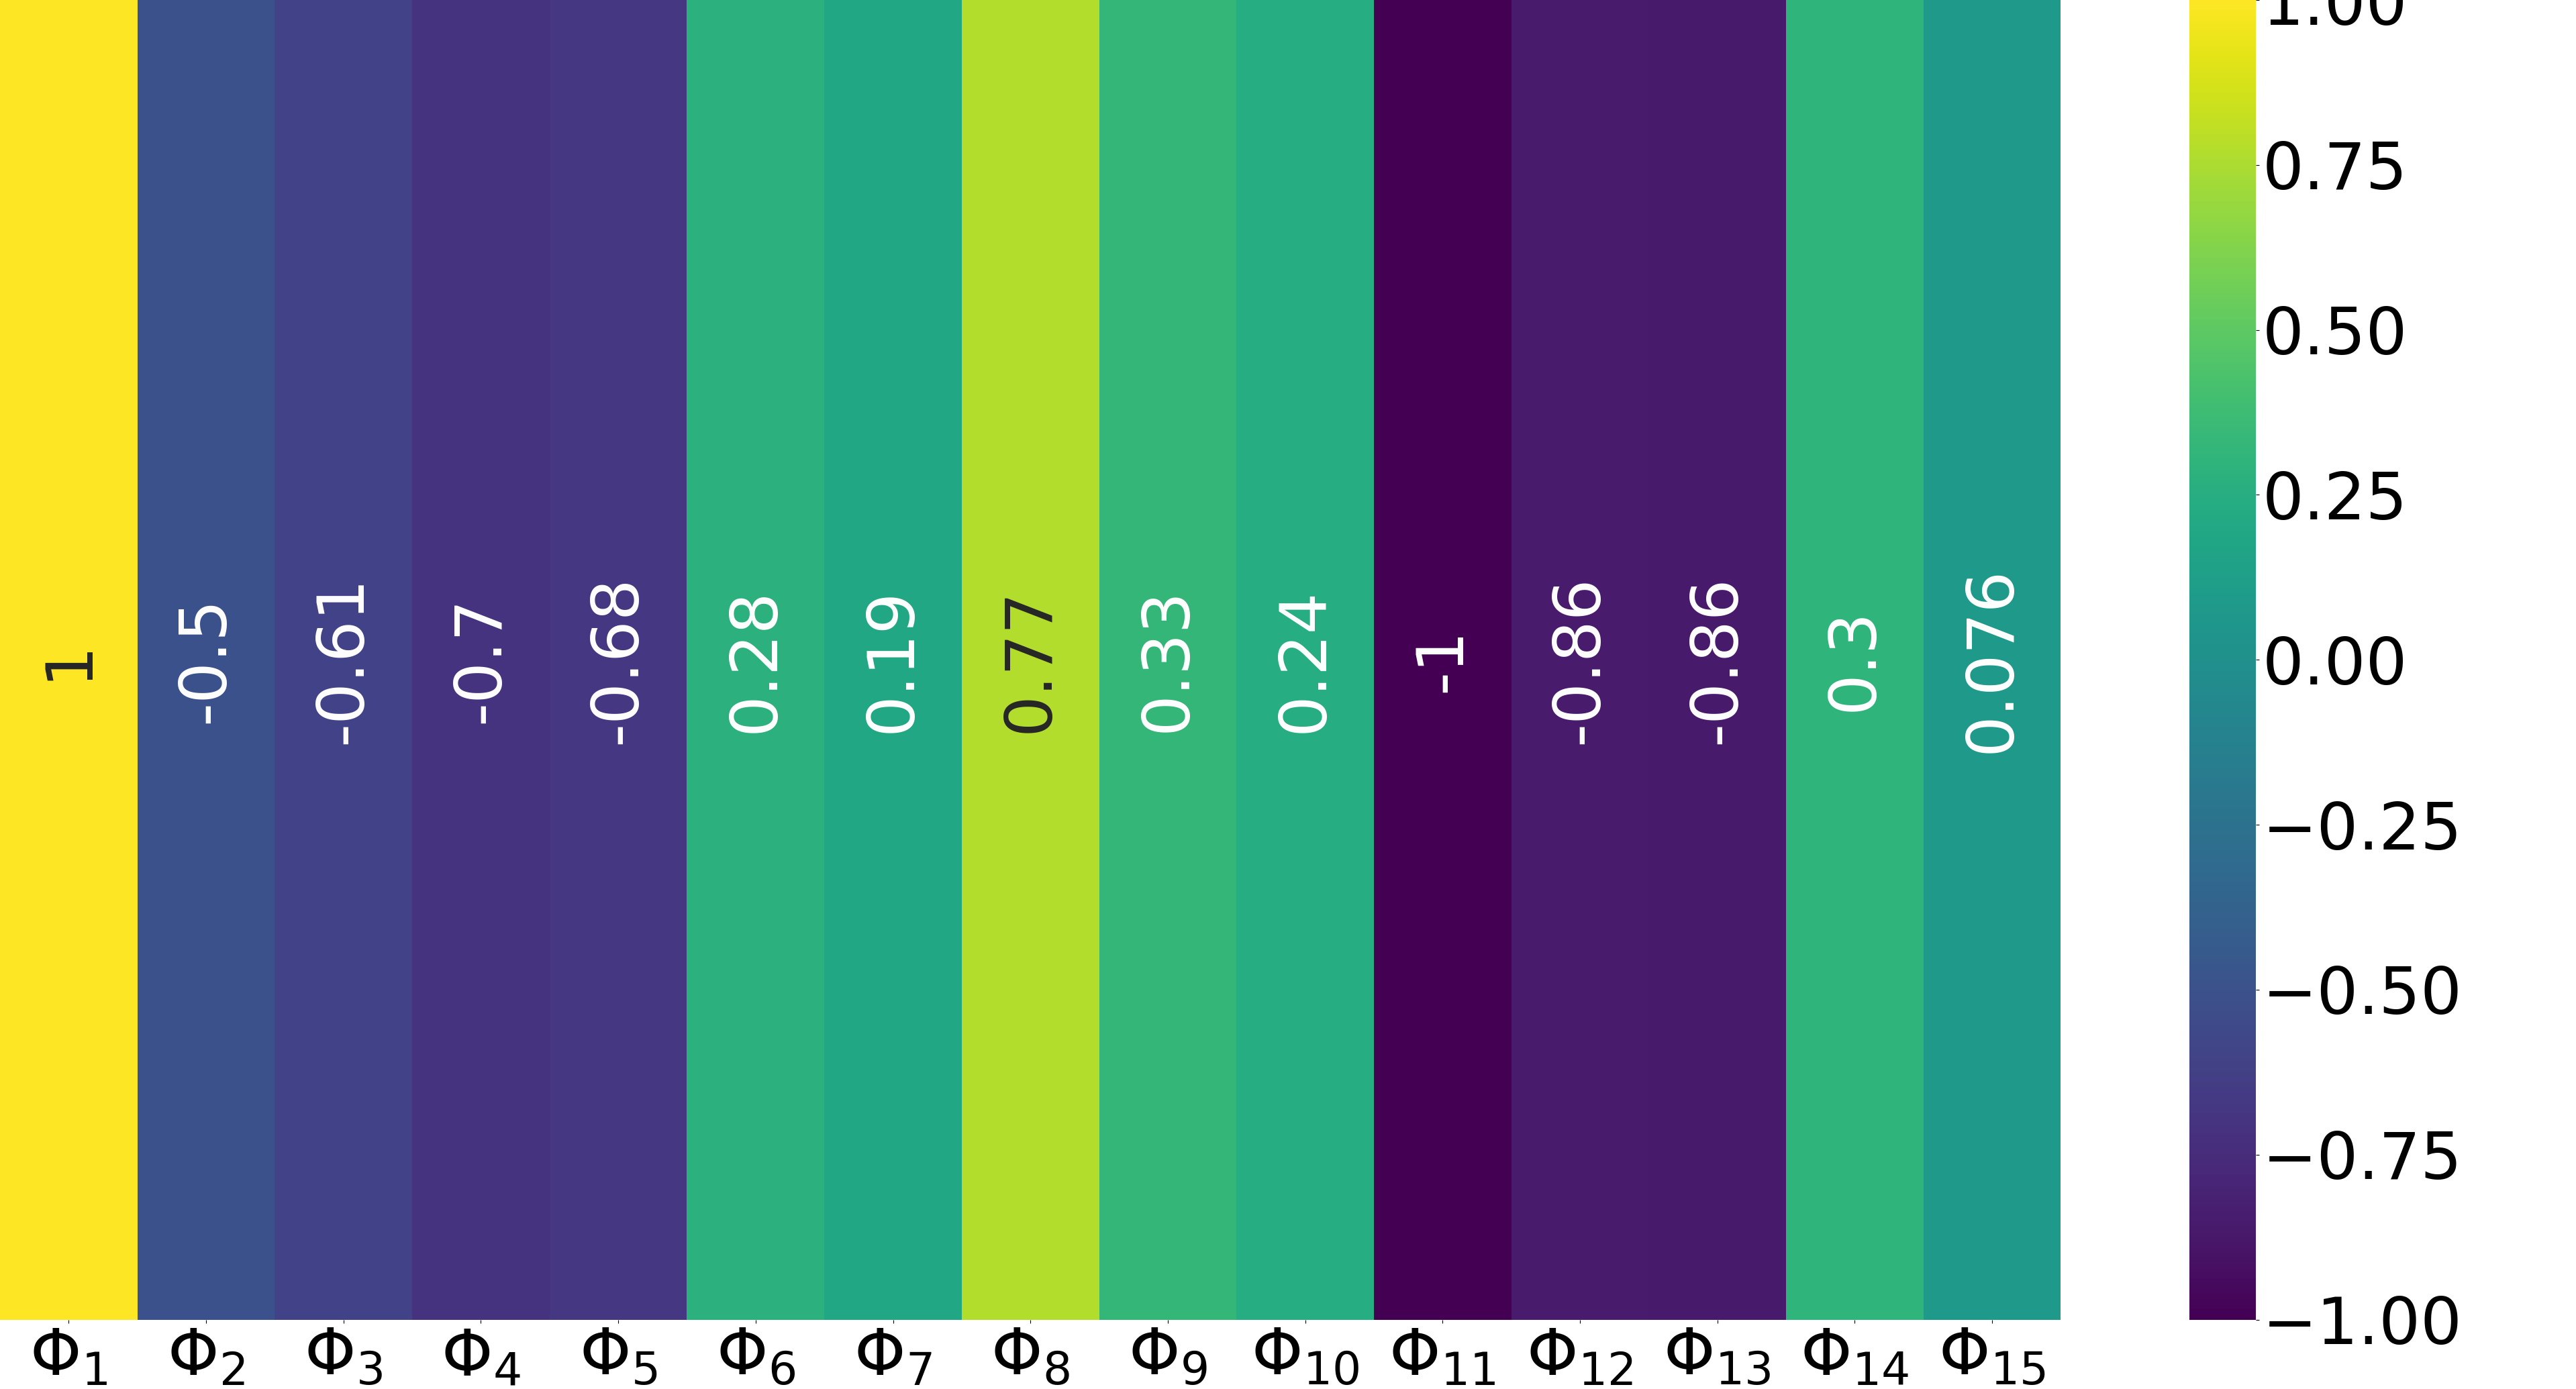
\includegraphics[width=\linewidth]{img/qlp_corr/Phi_coil0.png}
		\subcaption{Correlation with coil $0$}
	\end{subfigure}
	\begin{subfigure}{0.49\linewidth}
		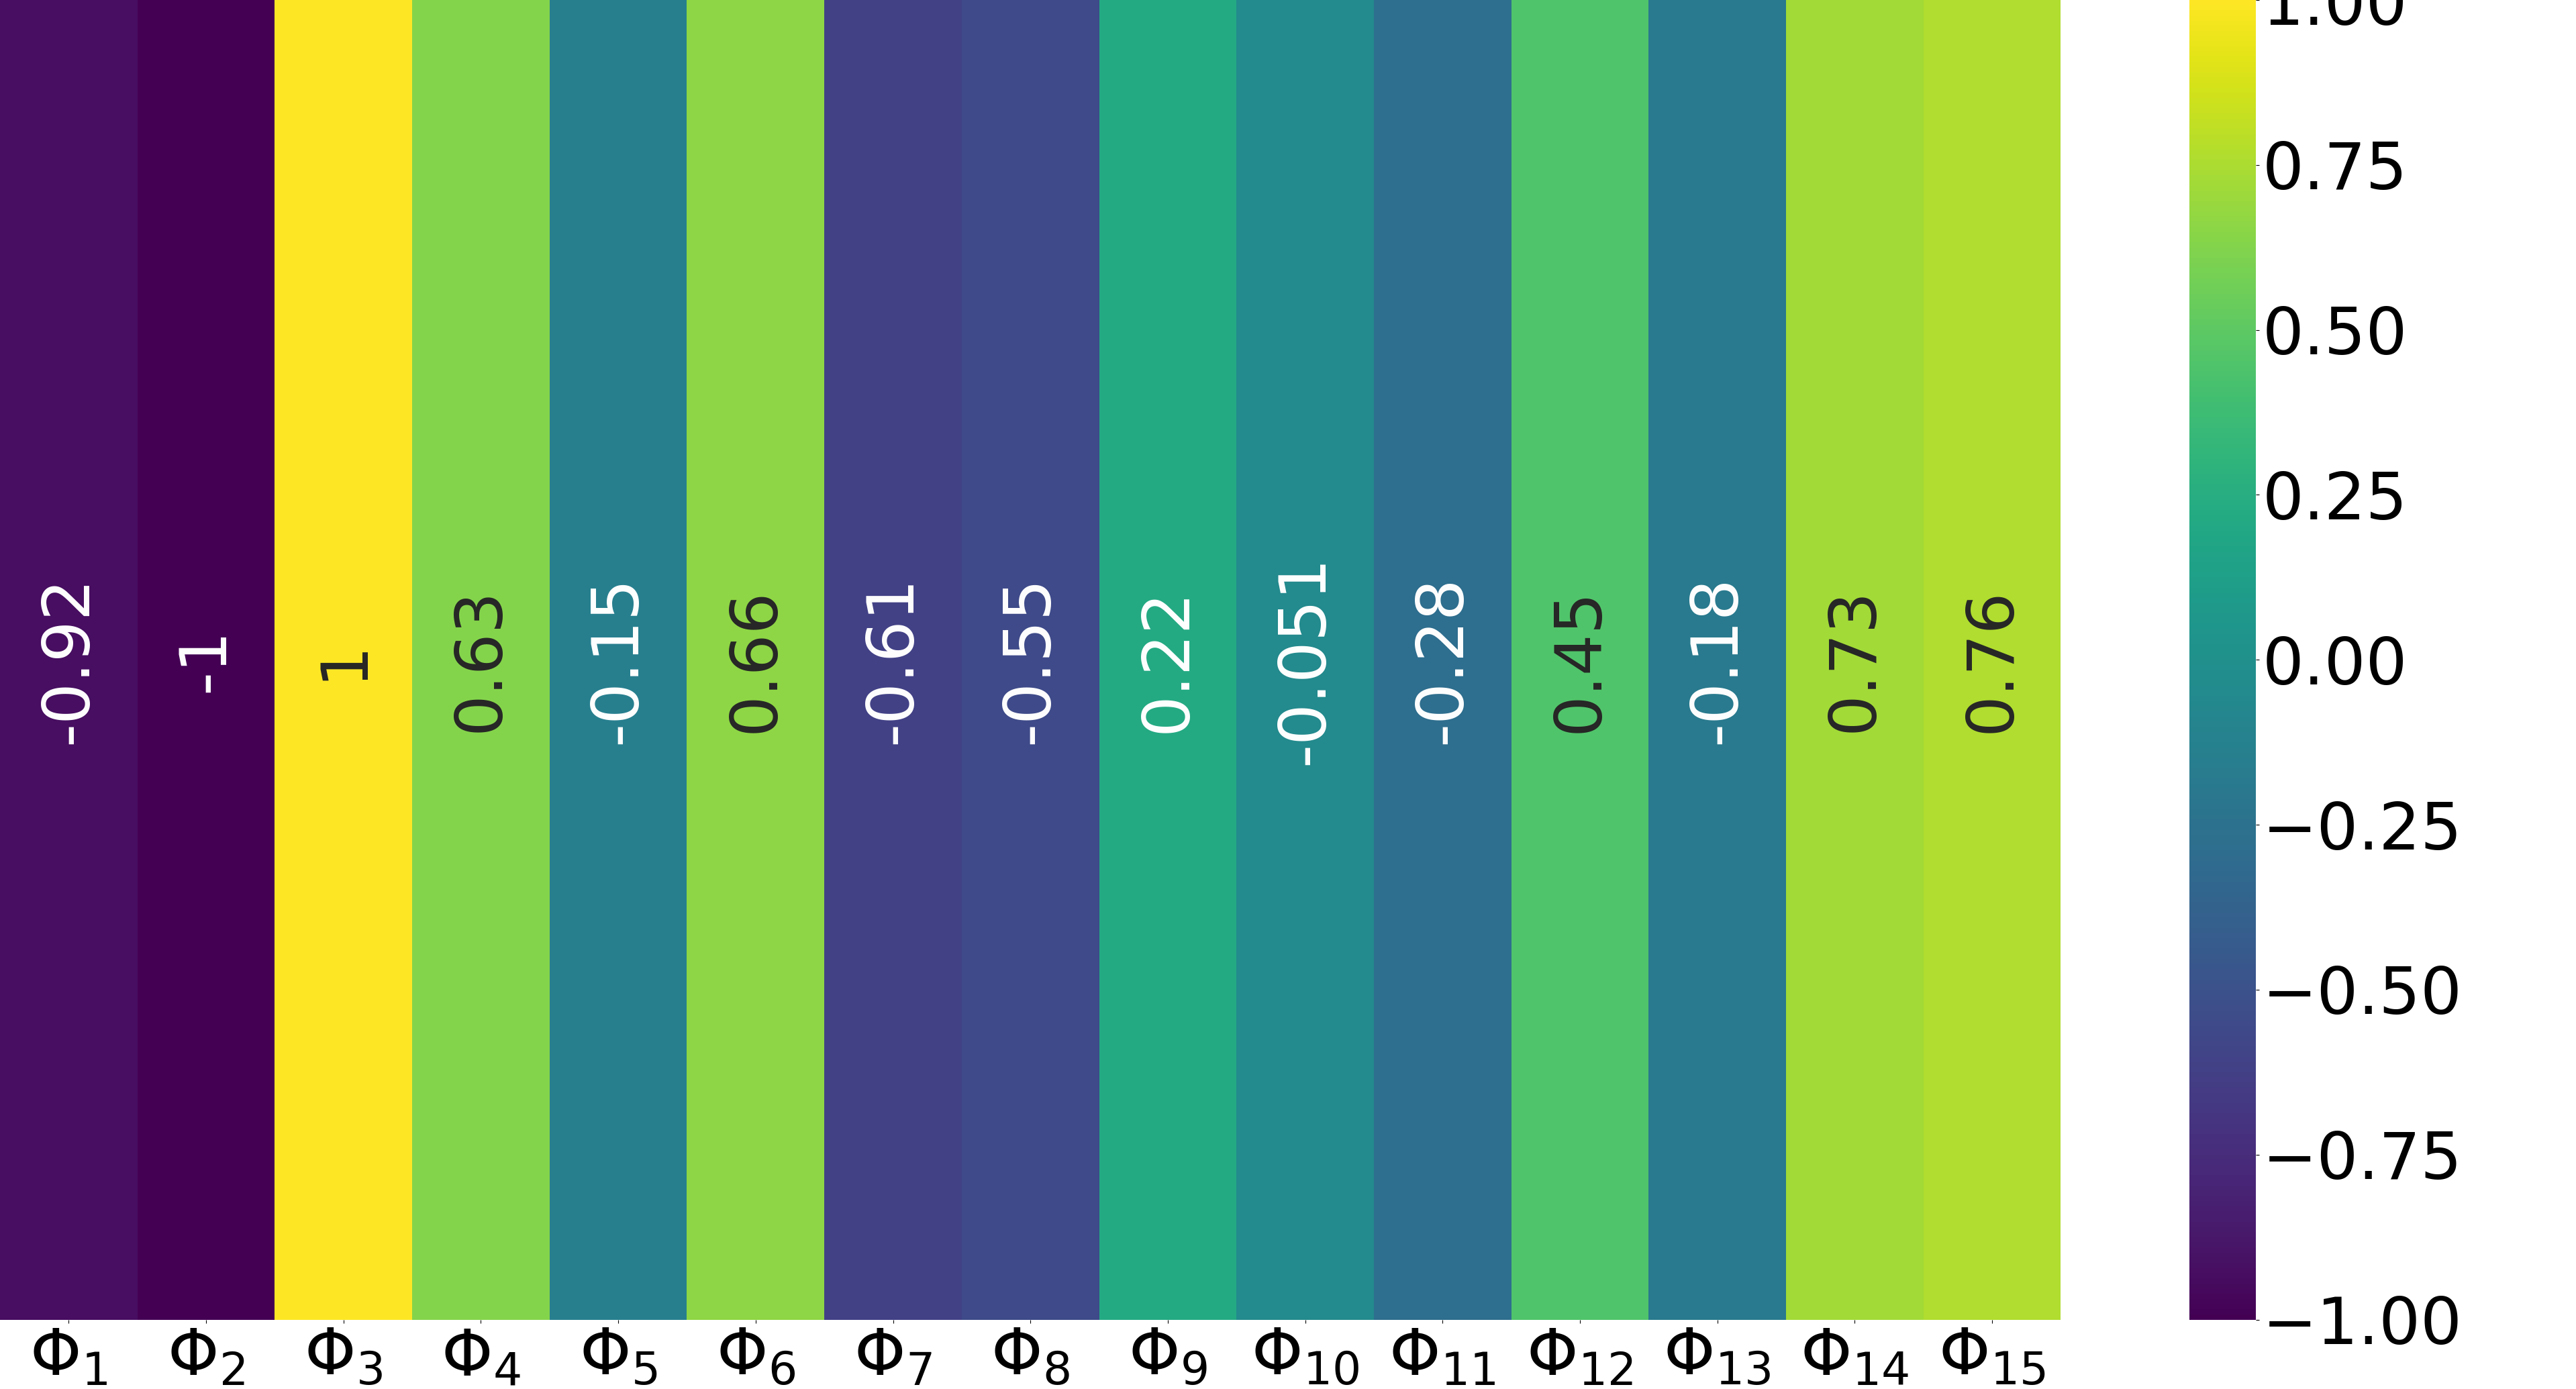
\includegraphics[width=\linewidth]{img/qlp_corr/Phi_coil1.png}
		\subcaption{Correlation with coil $1$}
	\end{subfigure}
	\begin{subfigure}{0.49\linewidth}
		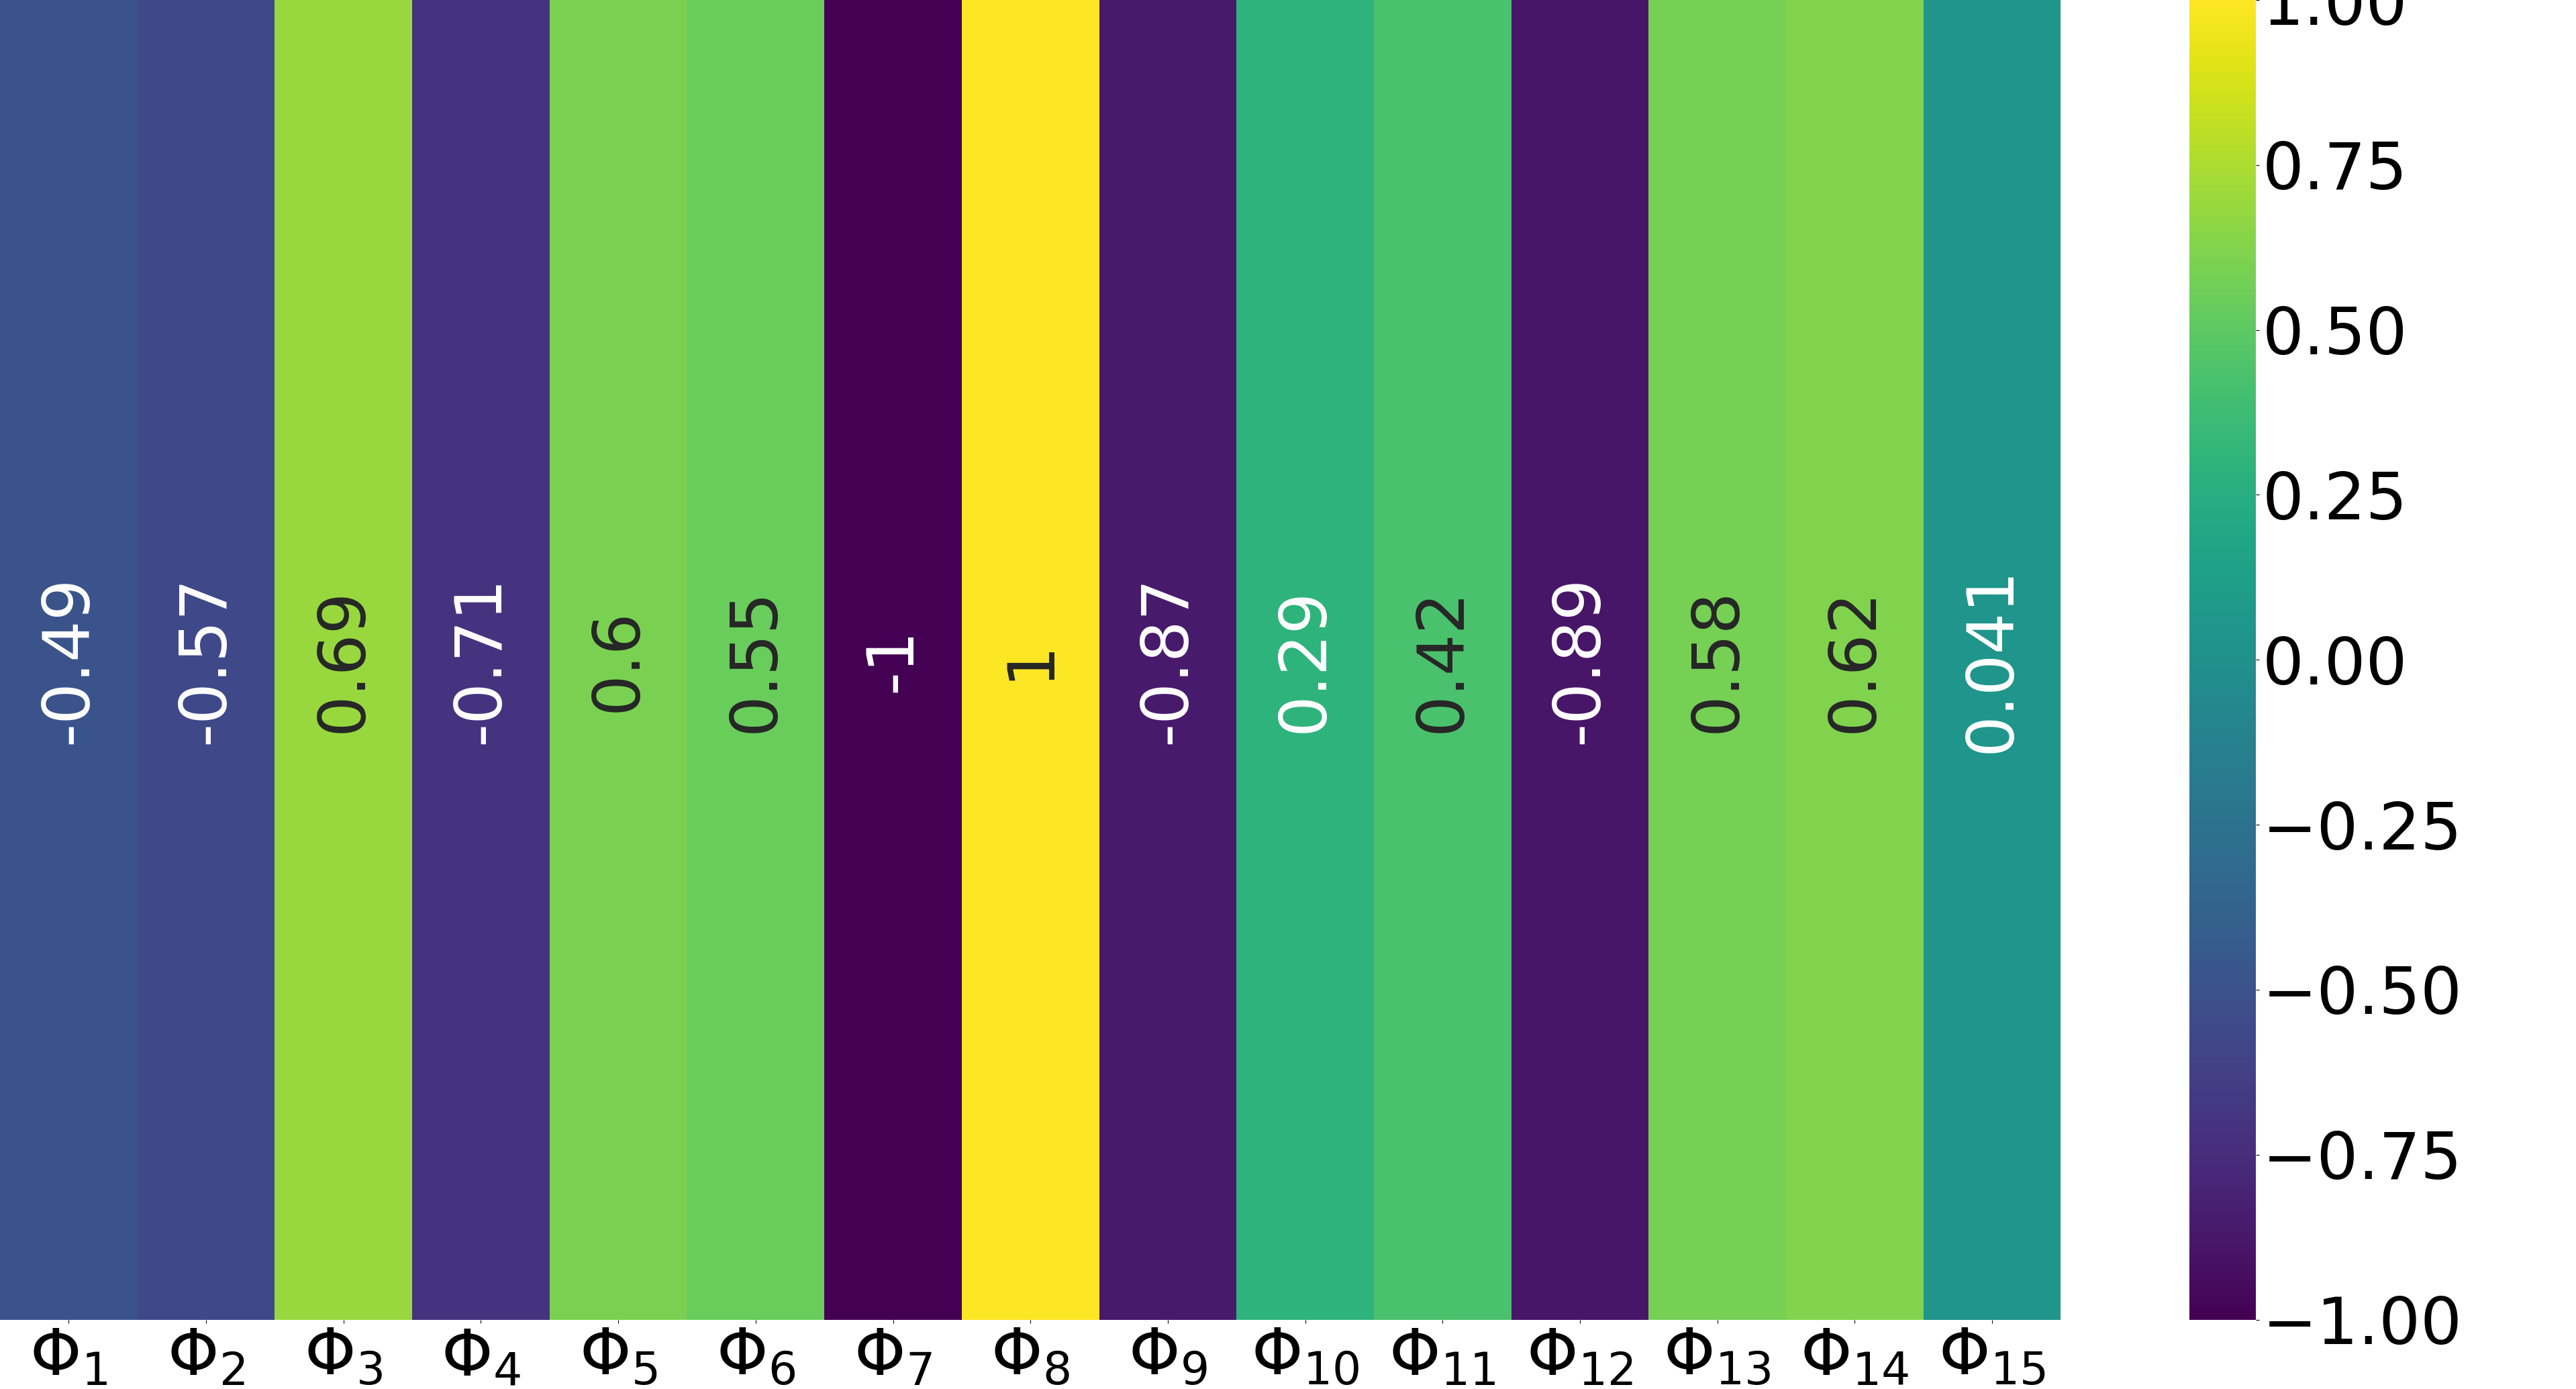
\includegraphics[width=\linewidth]{img/qlp_corr/Phi_coil2.png}
		\subcaption{Correlation with coil $2$}
	\end{subfigure}
	\begin{subfigure}{0.49\linewidth}
		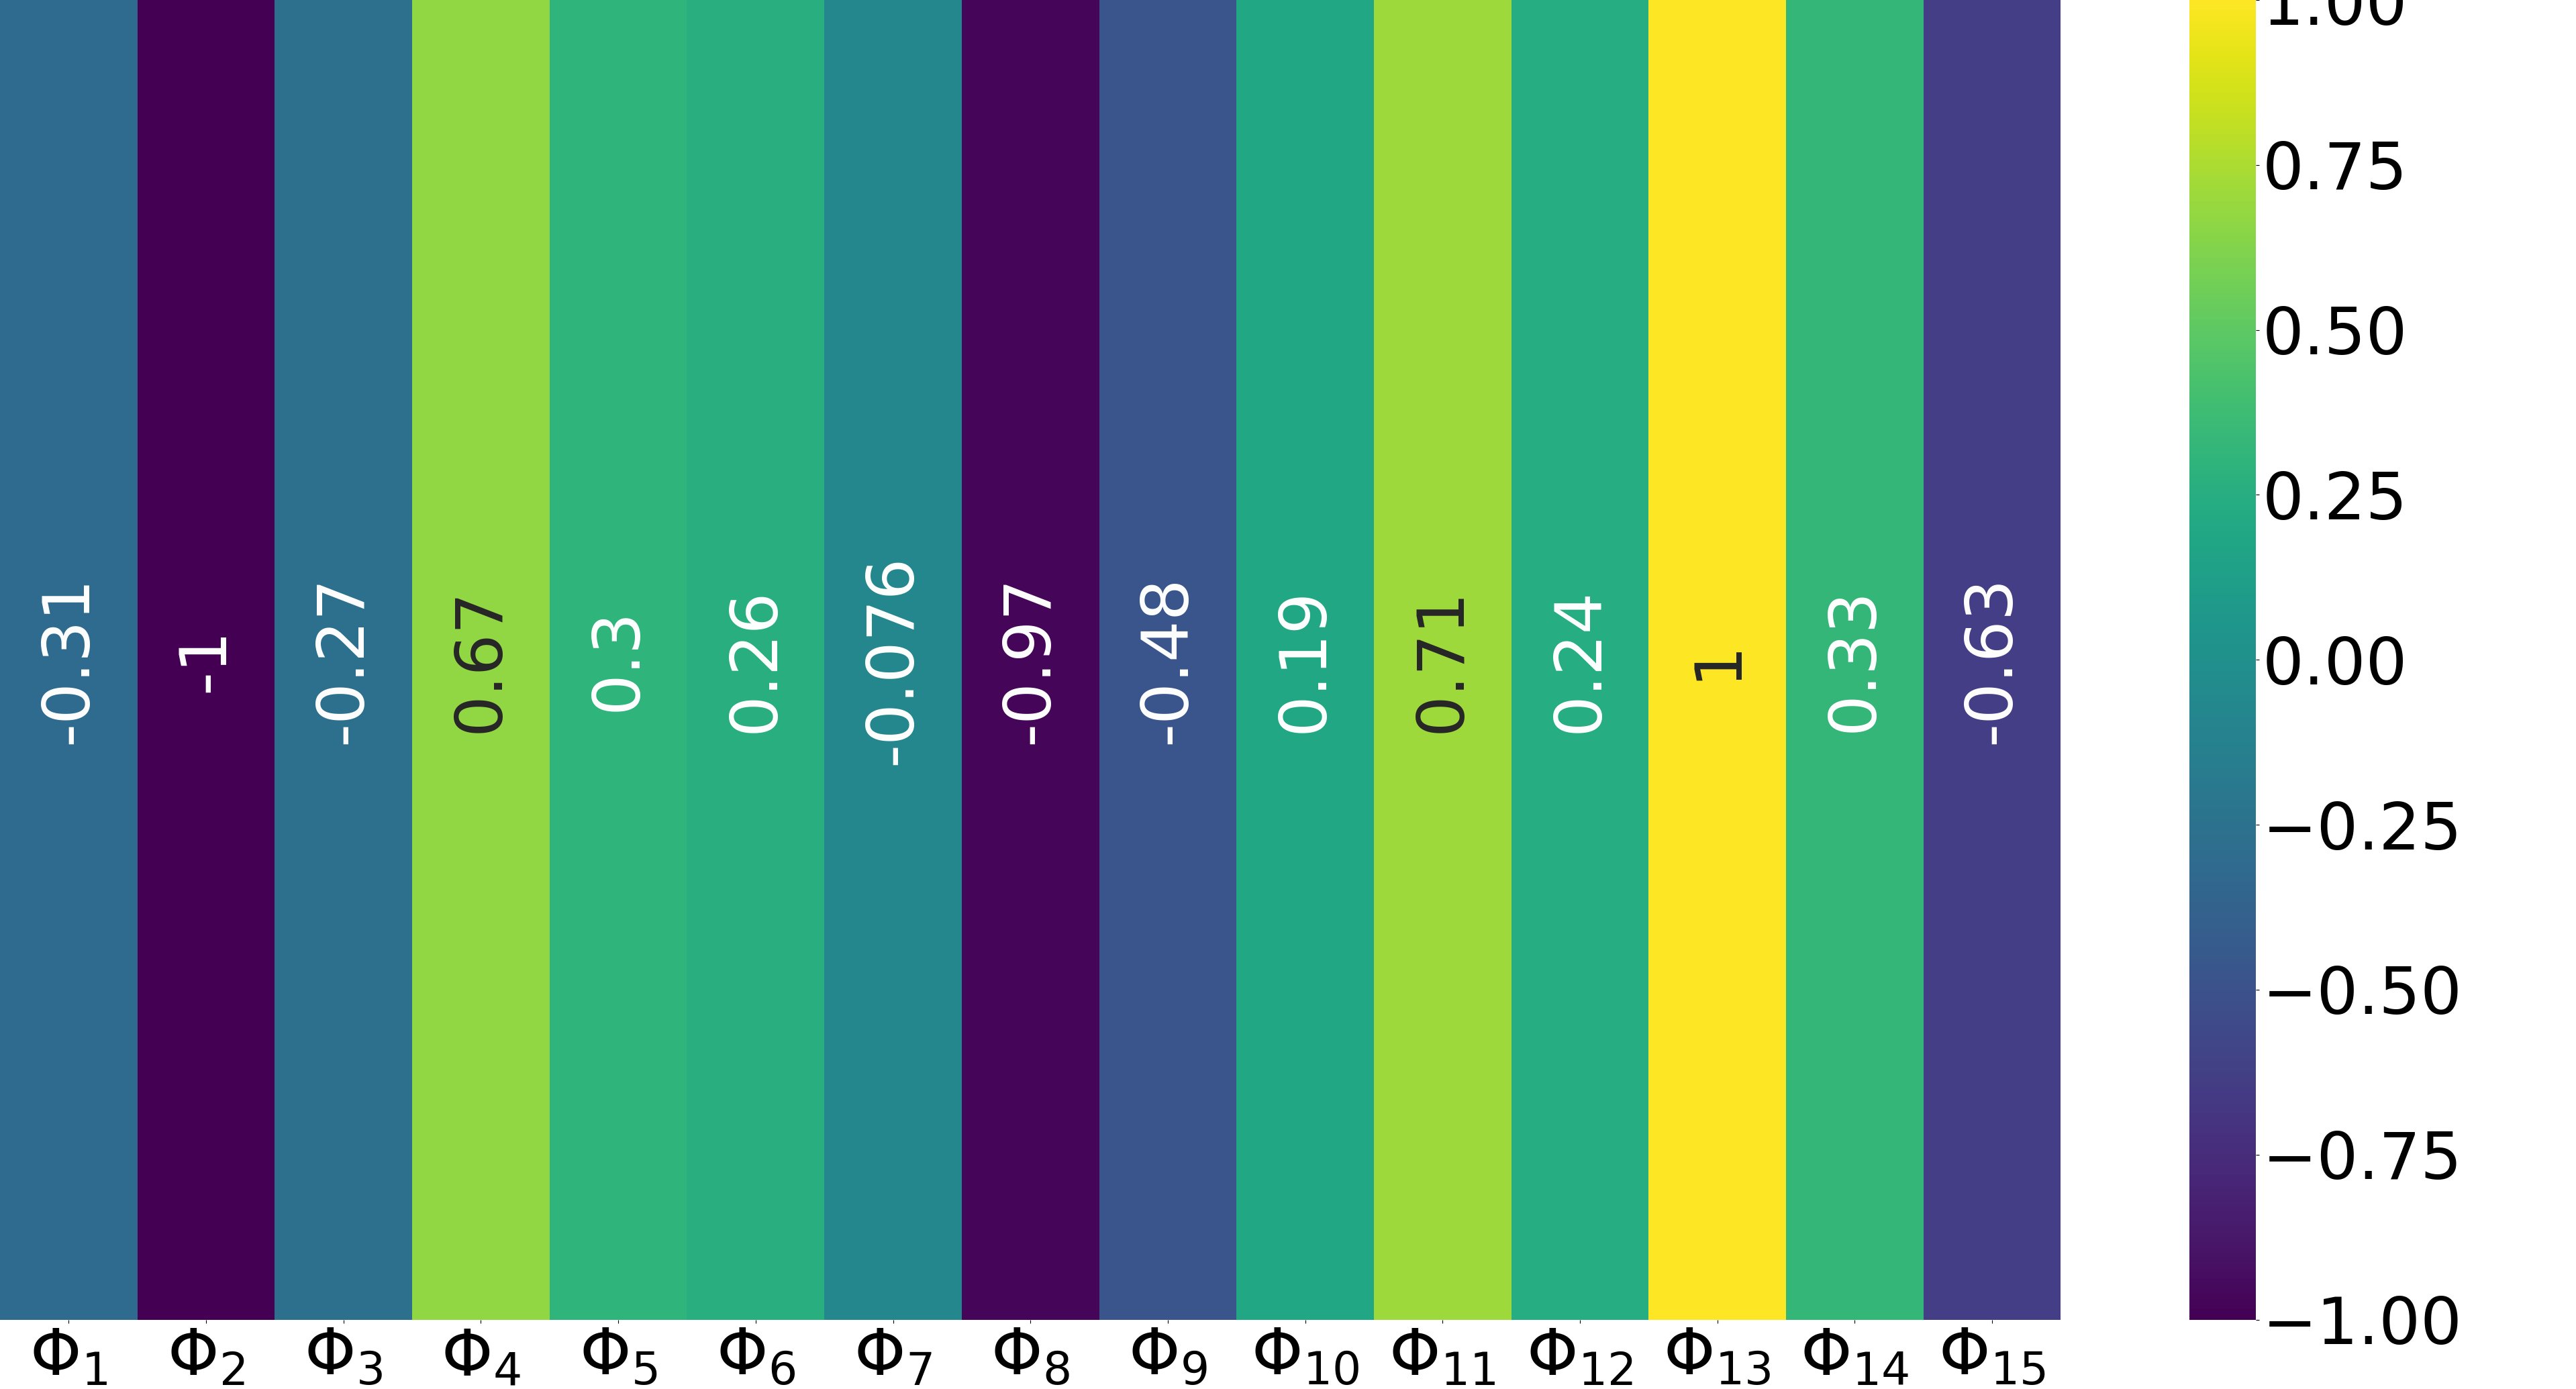
\includegraphics[width=\linewidth]{img/qlp_corr/Phi_coil3.png}
		\subcaption{Correlation with coil $3$}
	\end{subfigure}
	\caption{Correlation between the harmonics of the \phin\ attribute and the labels for \qlp.}
	\label{fig:phi-lcorr-qlp}
\end{figure}

On the other hand, the bidimensional visualization of the data is telling a different story (cfr.
\Cref{fig:phi-coilq-dist}), closer, as a matter of fact, to what we discovered for \bn. \Cref{fig:phi-coilq-dist} plots the data after a round of \pca\ dimensionality reduction. Independently of the sub-figure we consider, the sparsity and the homogeneity of the data makes it
extremely hard to define clusters with a high level of purity.
\begin{figure}[!ht]
	% Font size = 40
	\centering
	\begin{subfigure}{0.6\linewidth}
		\centering
		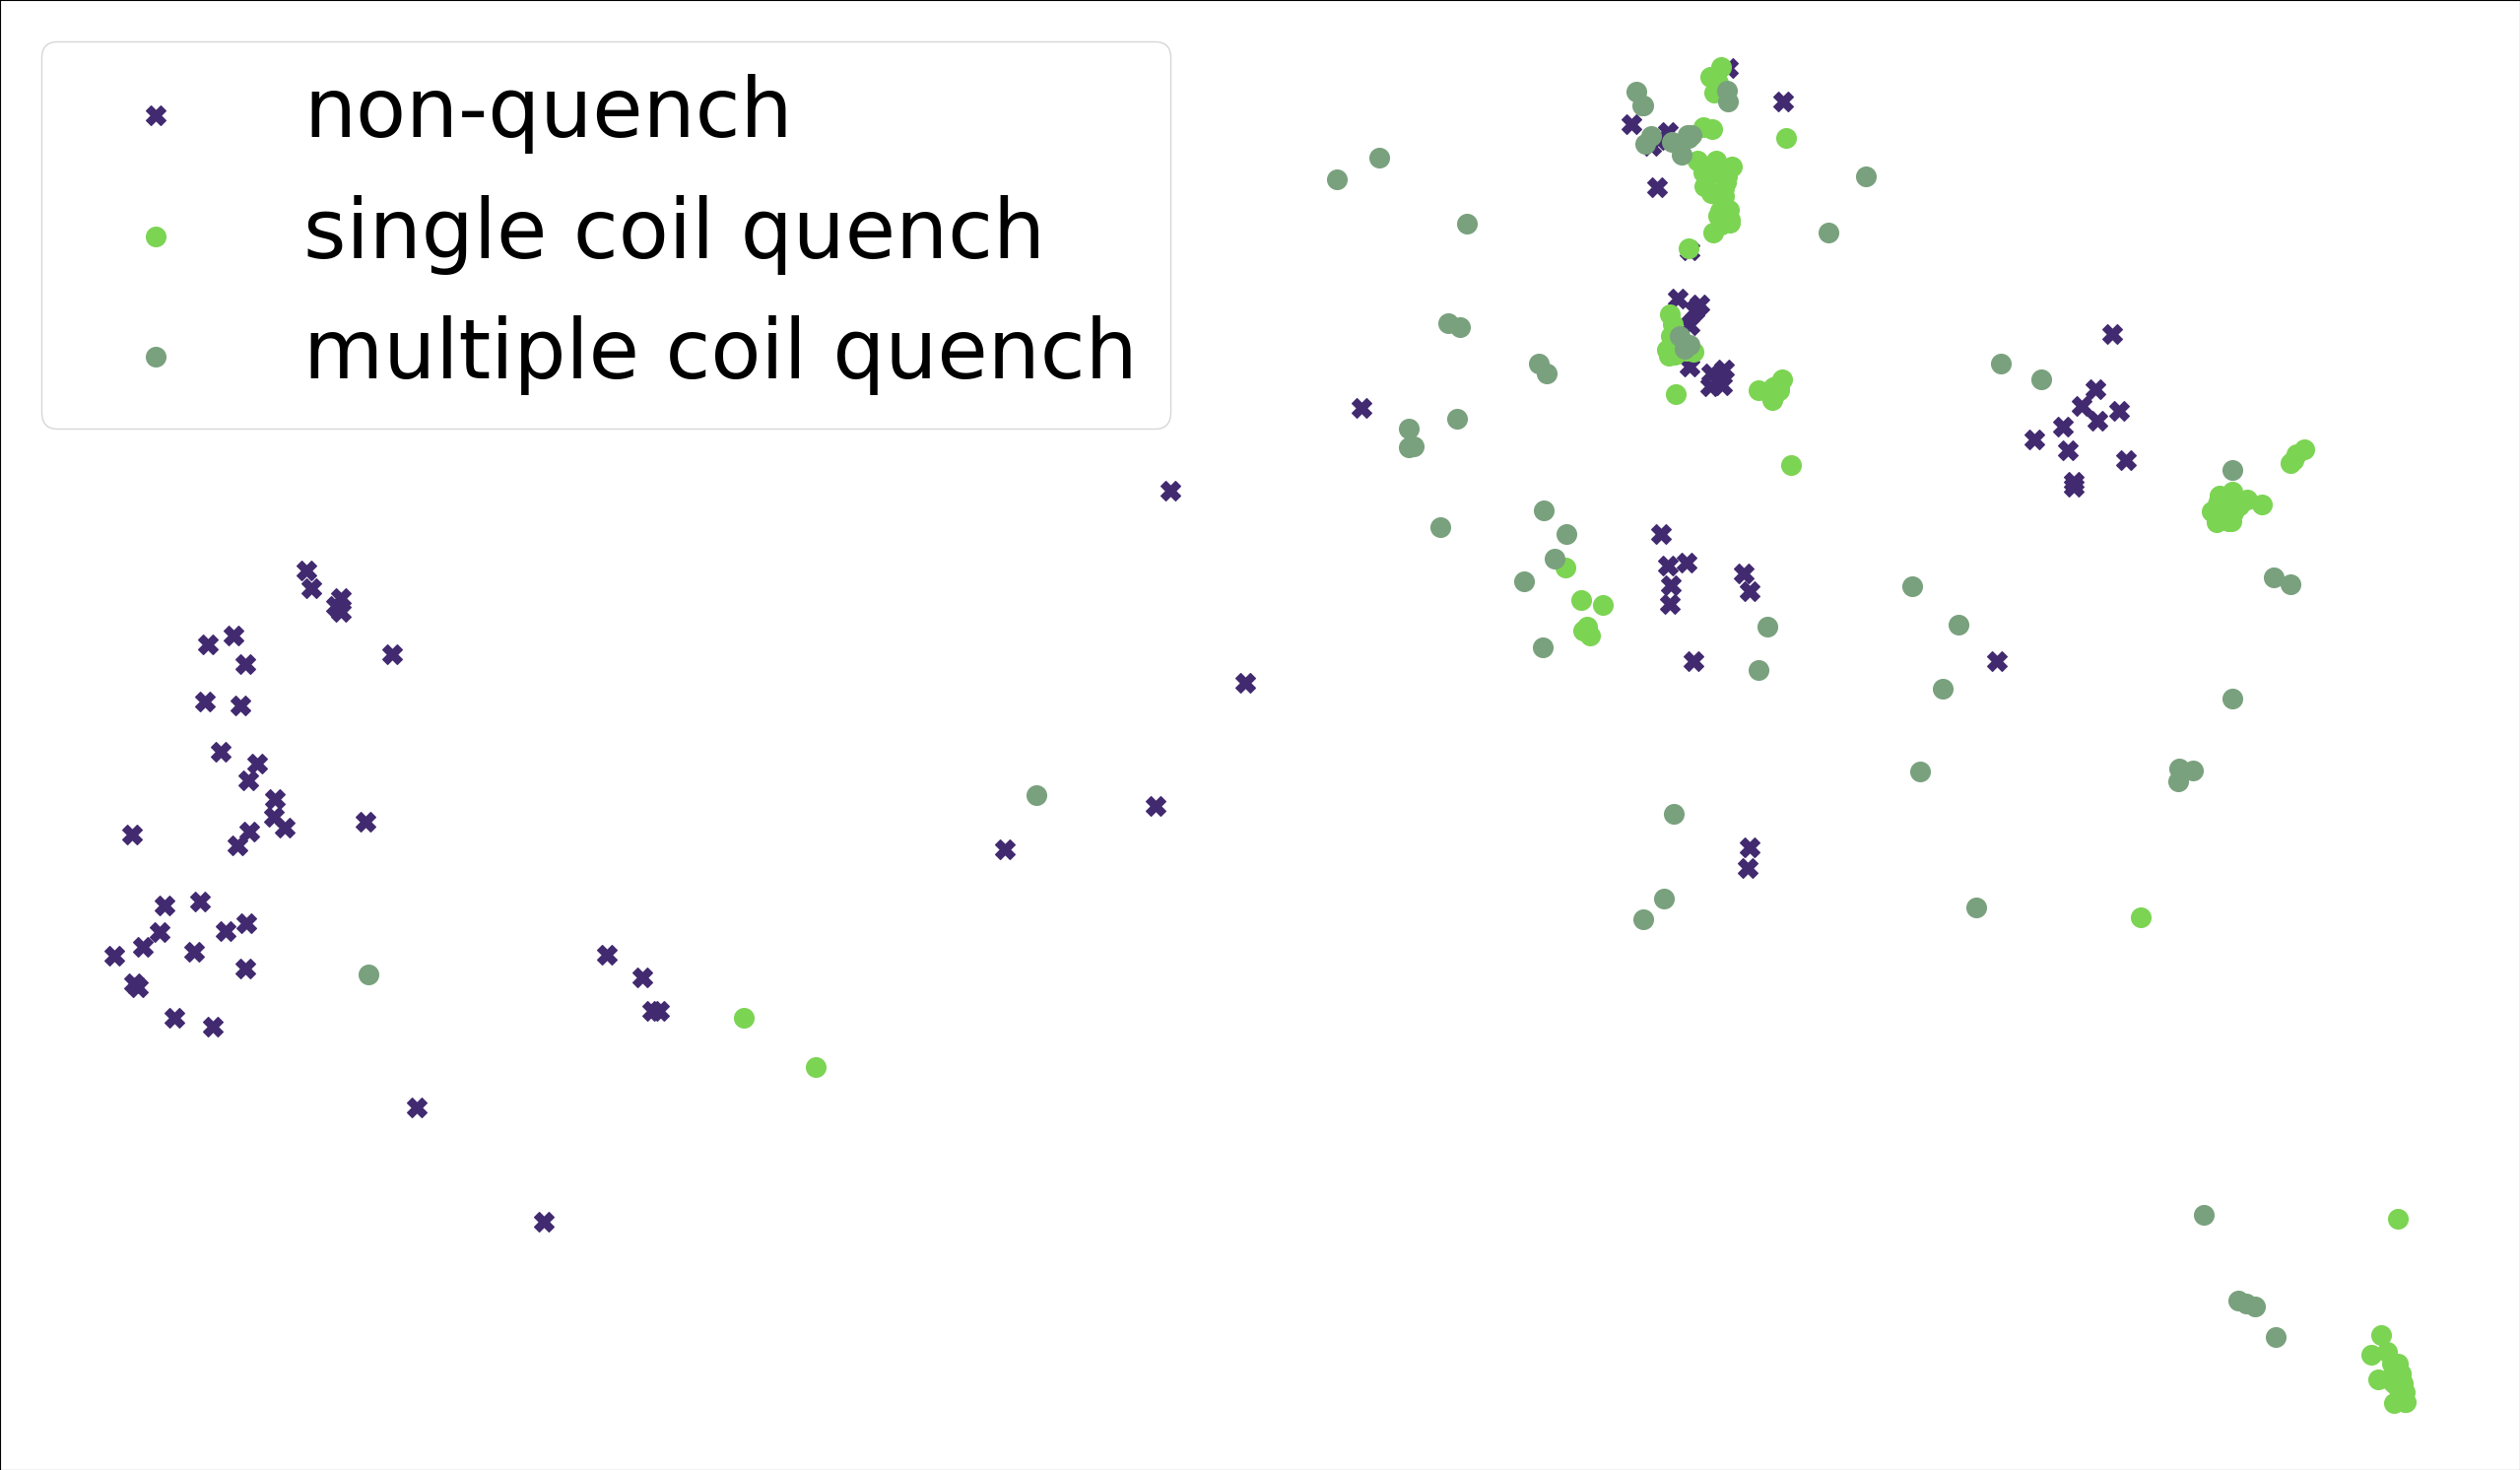
\includegraphics[width=\linewidth]{img/quench_dist_qlp/single_vs_multiple_Phi.png}
		\subcaption{}
	\end{subfigure}
	\begin{subfigure}{0.6\linewidth}
		\centering
		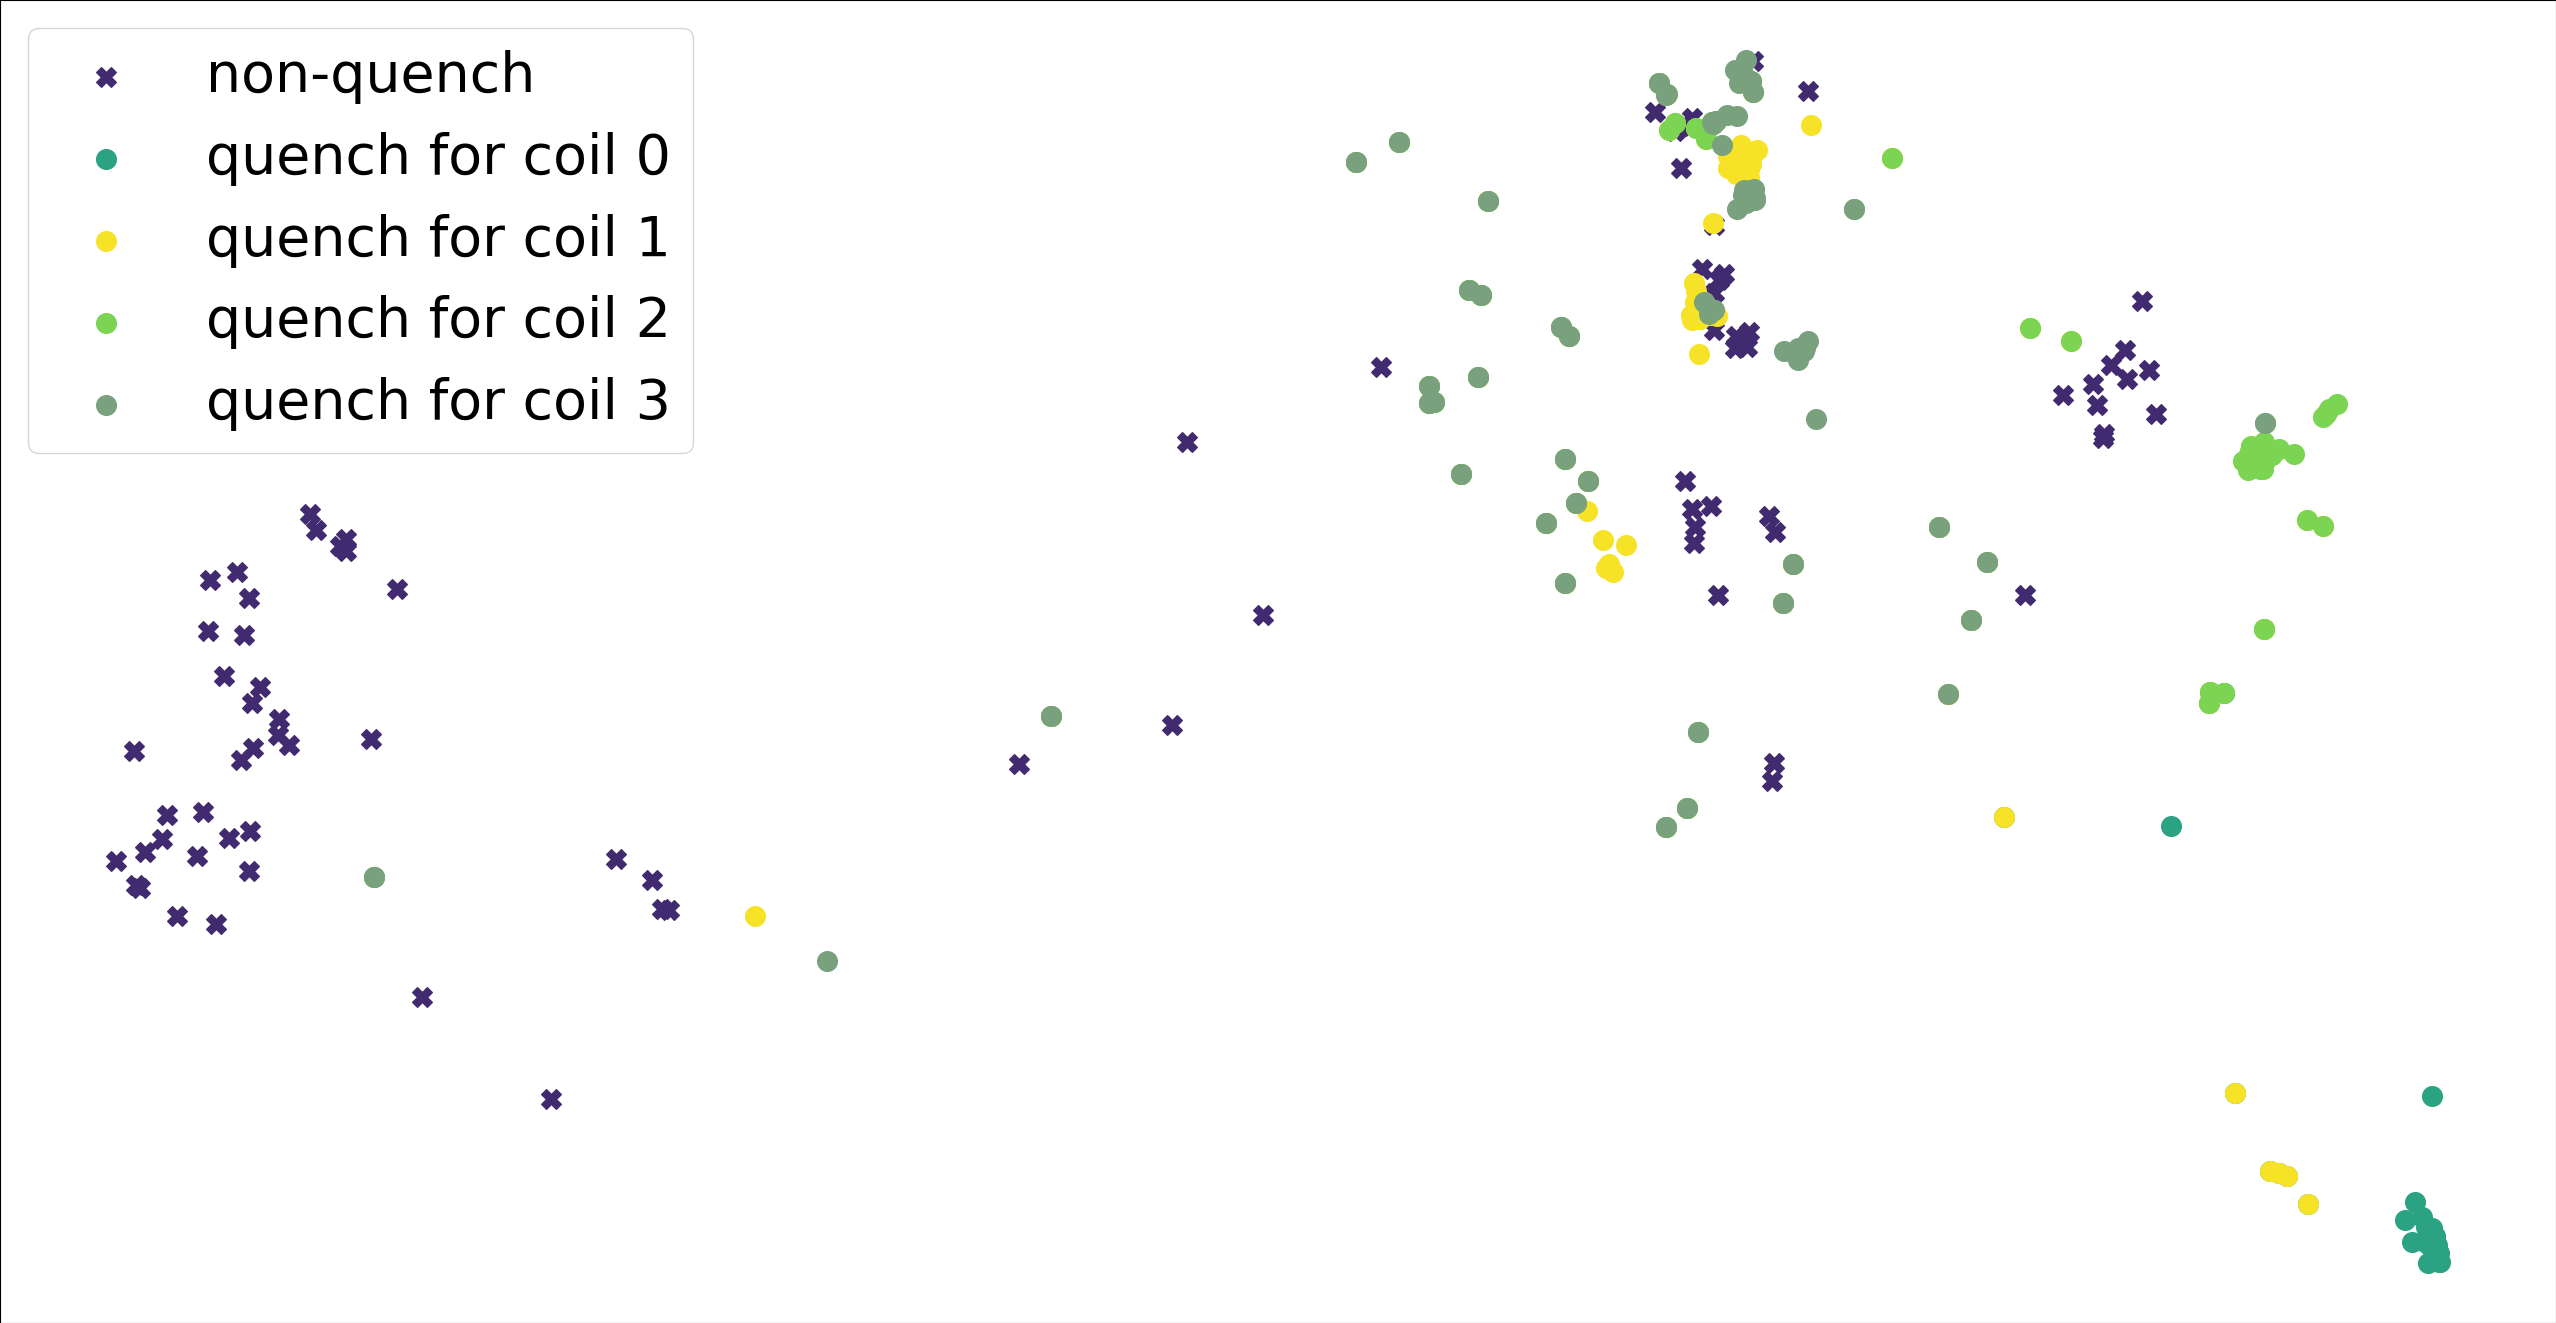
\includegraphics[width=\linewidth]{img/quench_dist_qlp_phi.png}
		\subcaption{}
	\end{subfigure}
	\caption{Visualization of the \phin\ attribute, the data was plotted after a run of \pca\
		dimensionality reduction. Sub-figure (a) highlights the samples based on how many quenches
		are associated to the specific sample $\{0, 1, \text{many}\}$. Sub-figure (b) highlights the
		samples based on the specific coil quenched $\{\text{None}, 0, 1, 2, 3\}$.}
	\label{fig:phi-coilq-dist}
\end{figure}

\section{First approaches using Clustering}
\label{sec:qlp-cluster}
In the previous sections and in the original preprocessing we did for \qrp\ (see
\Cref{sec:qrp-preprocessing}), we hinted more than once at the fact that both \an\ and \cnmod\ data was scattered favorably in
bidimensional space. We hoped that clustering on these attributes would yield unexpected insights
for \qlp, giving us a very early glimpse of undiscovered patterns in the data.

We remark that the $k$-means (see \Cref{sec:kmeans} for a theoretical introduction to the matter)
algorithm is always working by using distance between samples, therefore the pattern that it's
capable of identifying is unknown to us. Our job is to give a logic to the separation the algorithm
is finding in the data. We thought that a clustering approach could yield interesting results
because, by looking at the scattering of the data, it was very easy for us to identify a
partitioning of the space that yielded a semantically strong (although incomplete for some of our
pourposes) division.

We tried $k$-means clustering on all attributes, but we will only show relevant results. Data was plotted using \pca, but we also explored other dimensionality reduction techniques, namely FastICA~\footnote{
	ICA is a technique that tries to find a linear representation of non-Gaussian data so that
	the components are statistically independent, or as independent as possible~\cite{hyvarinen2000-fastICA}.
} and metric MultiDimensional Scaling (MDS)~\footnote{
	MultiDimensional Scaling is a technique used to define similarity or dissimilarity within a
	set of objects, and it does so by defining a distance among poiints in geometric space.
	There are many different types of MultiDimensional Scaling techniques, the main difference
	between them is the type of space that is being considered (e.g., Metric
	MDS)~\cite{Borg2005-metricMDS}.
}, generally yielding inferior results.

\begin{figure}[!ht]
	\centering
	\begin{subfigure}{0.6\linewidth}
		\centering
		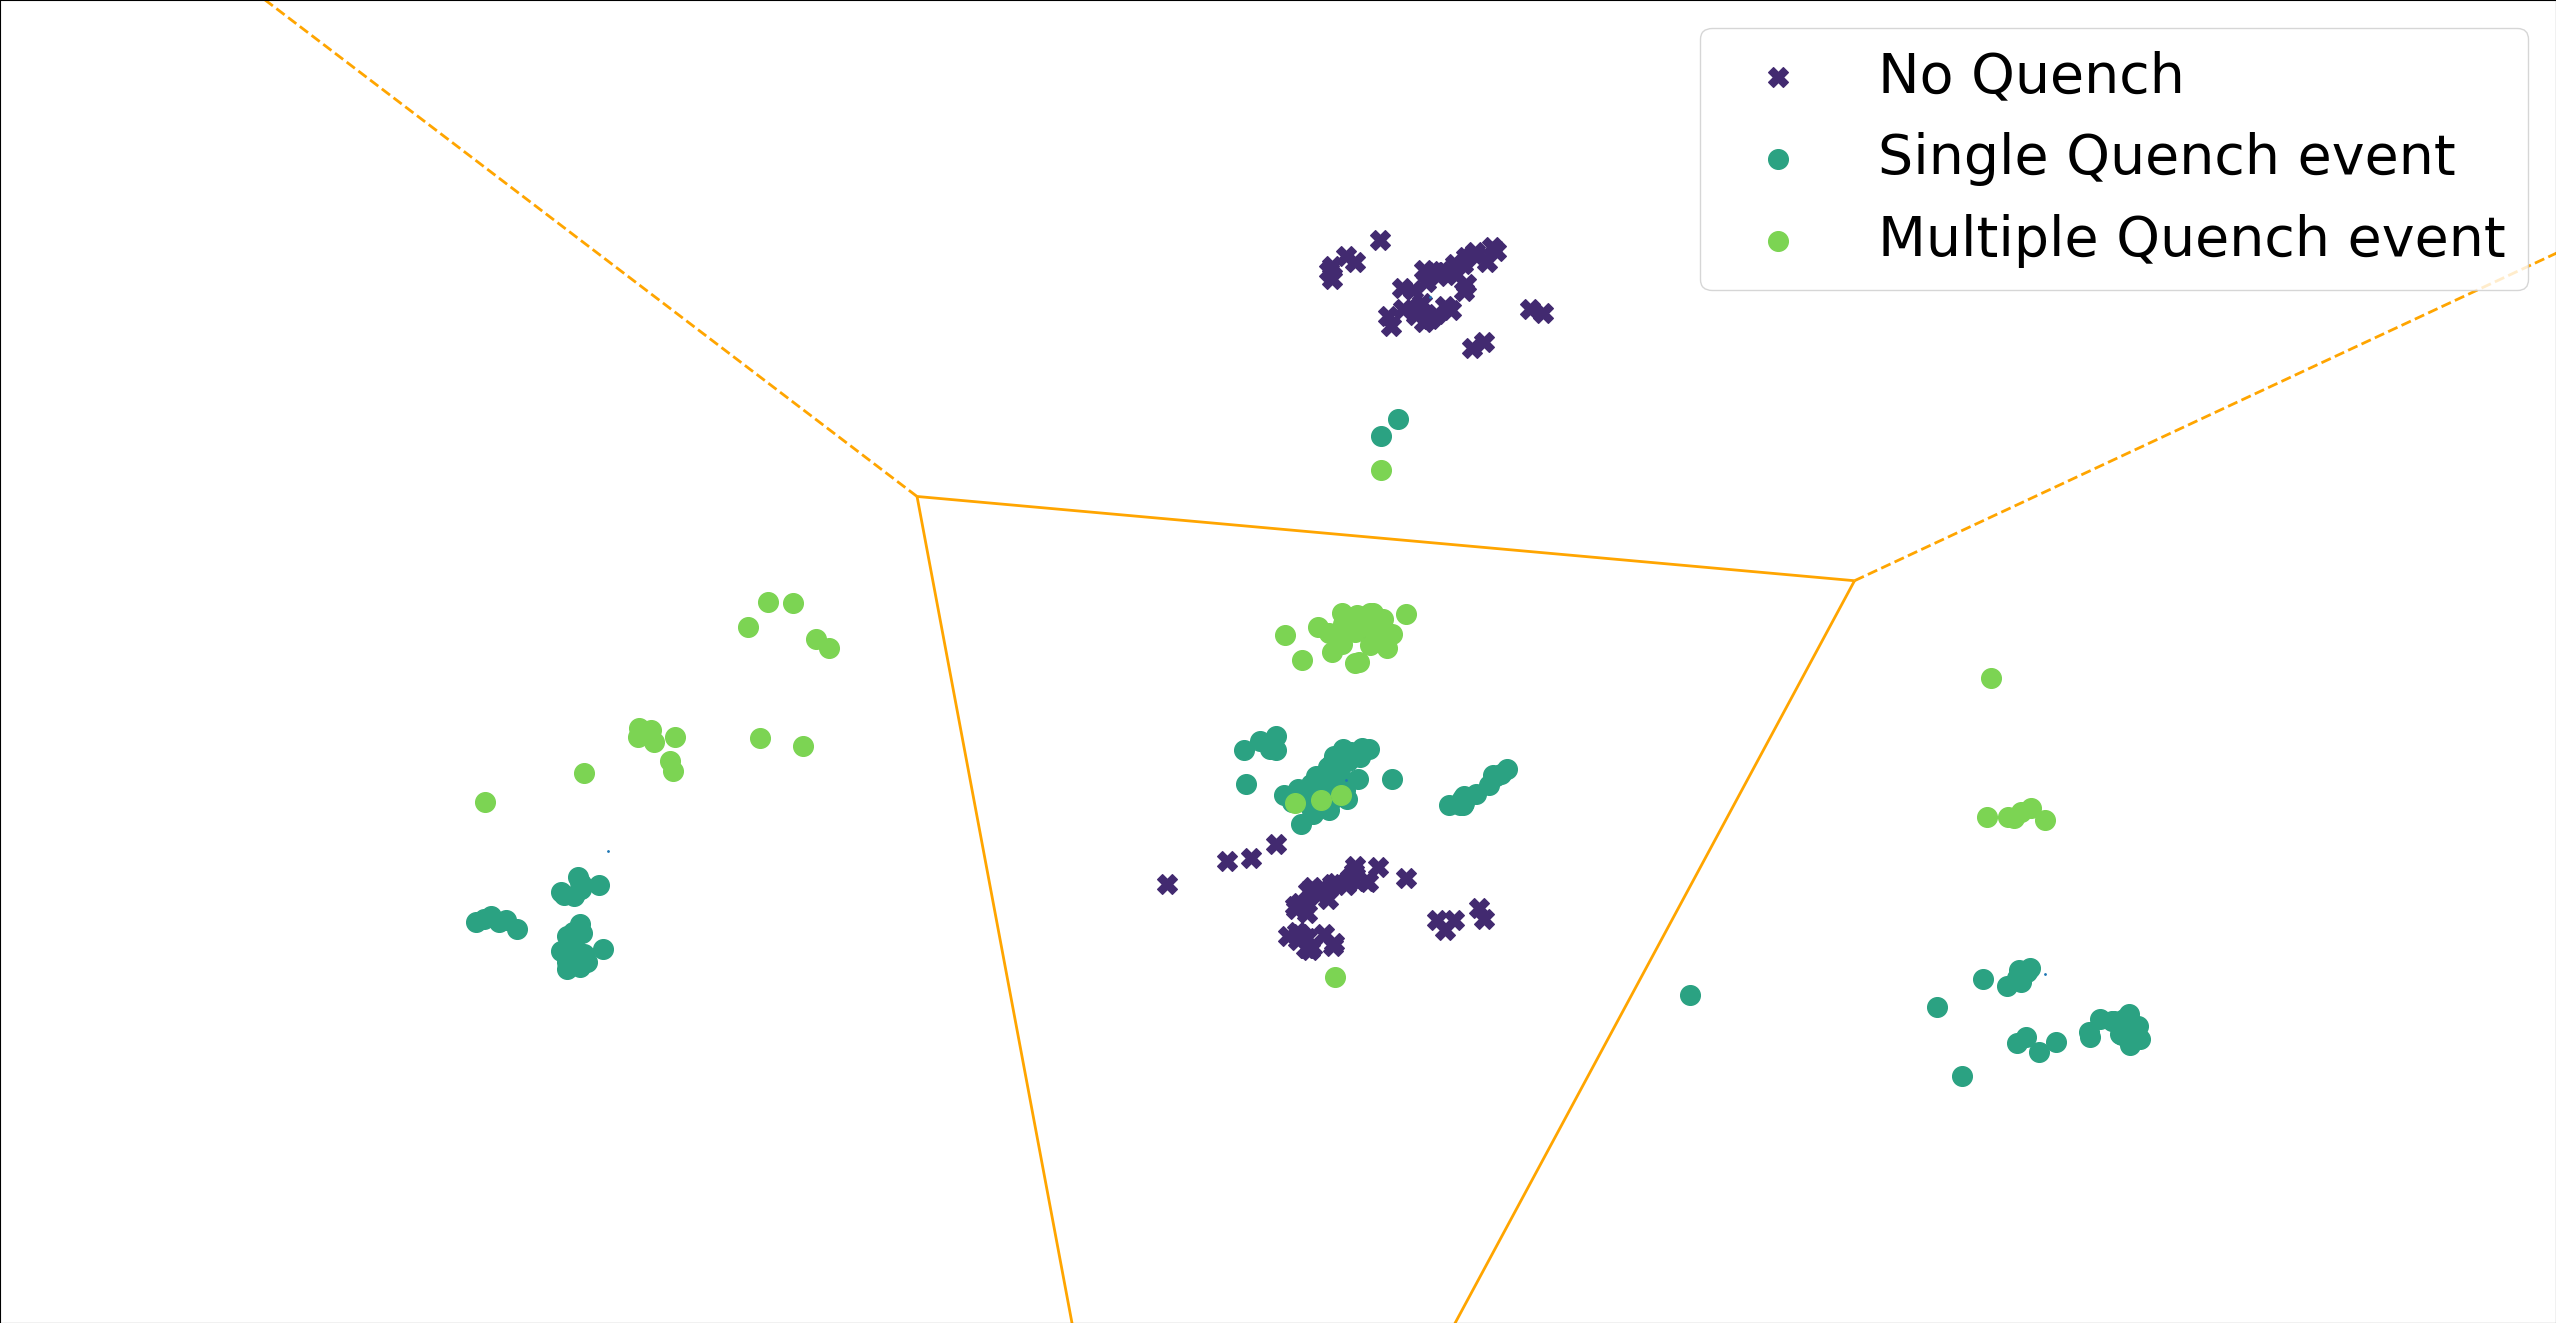
\includegraphics[width=\linewidth]{img/clustering_an_qlp_4c.png}
		\caption{$4$-means clustering on \an.}
	\end{subfigure}
	\begin{subfigure}{0.6\linewidth}
		\centering
		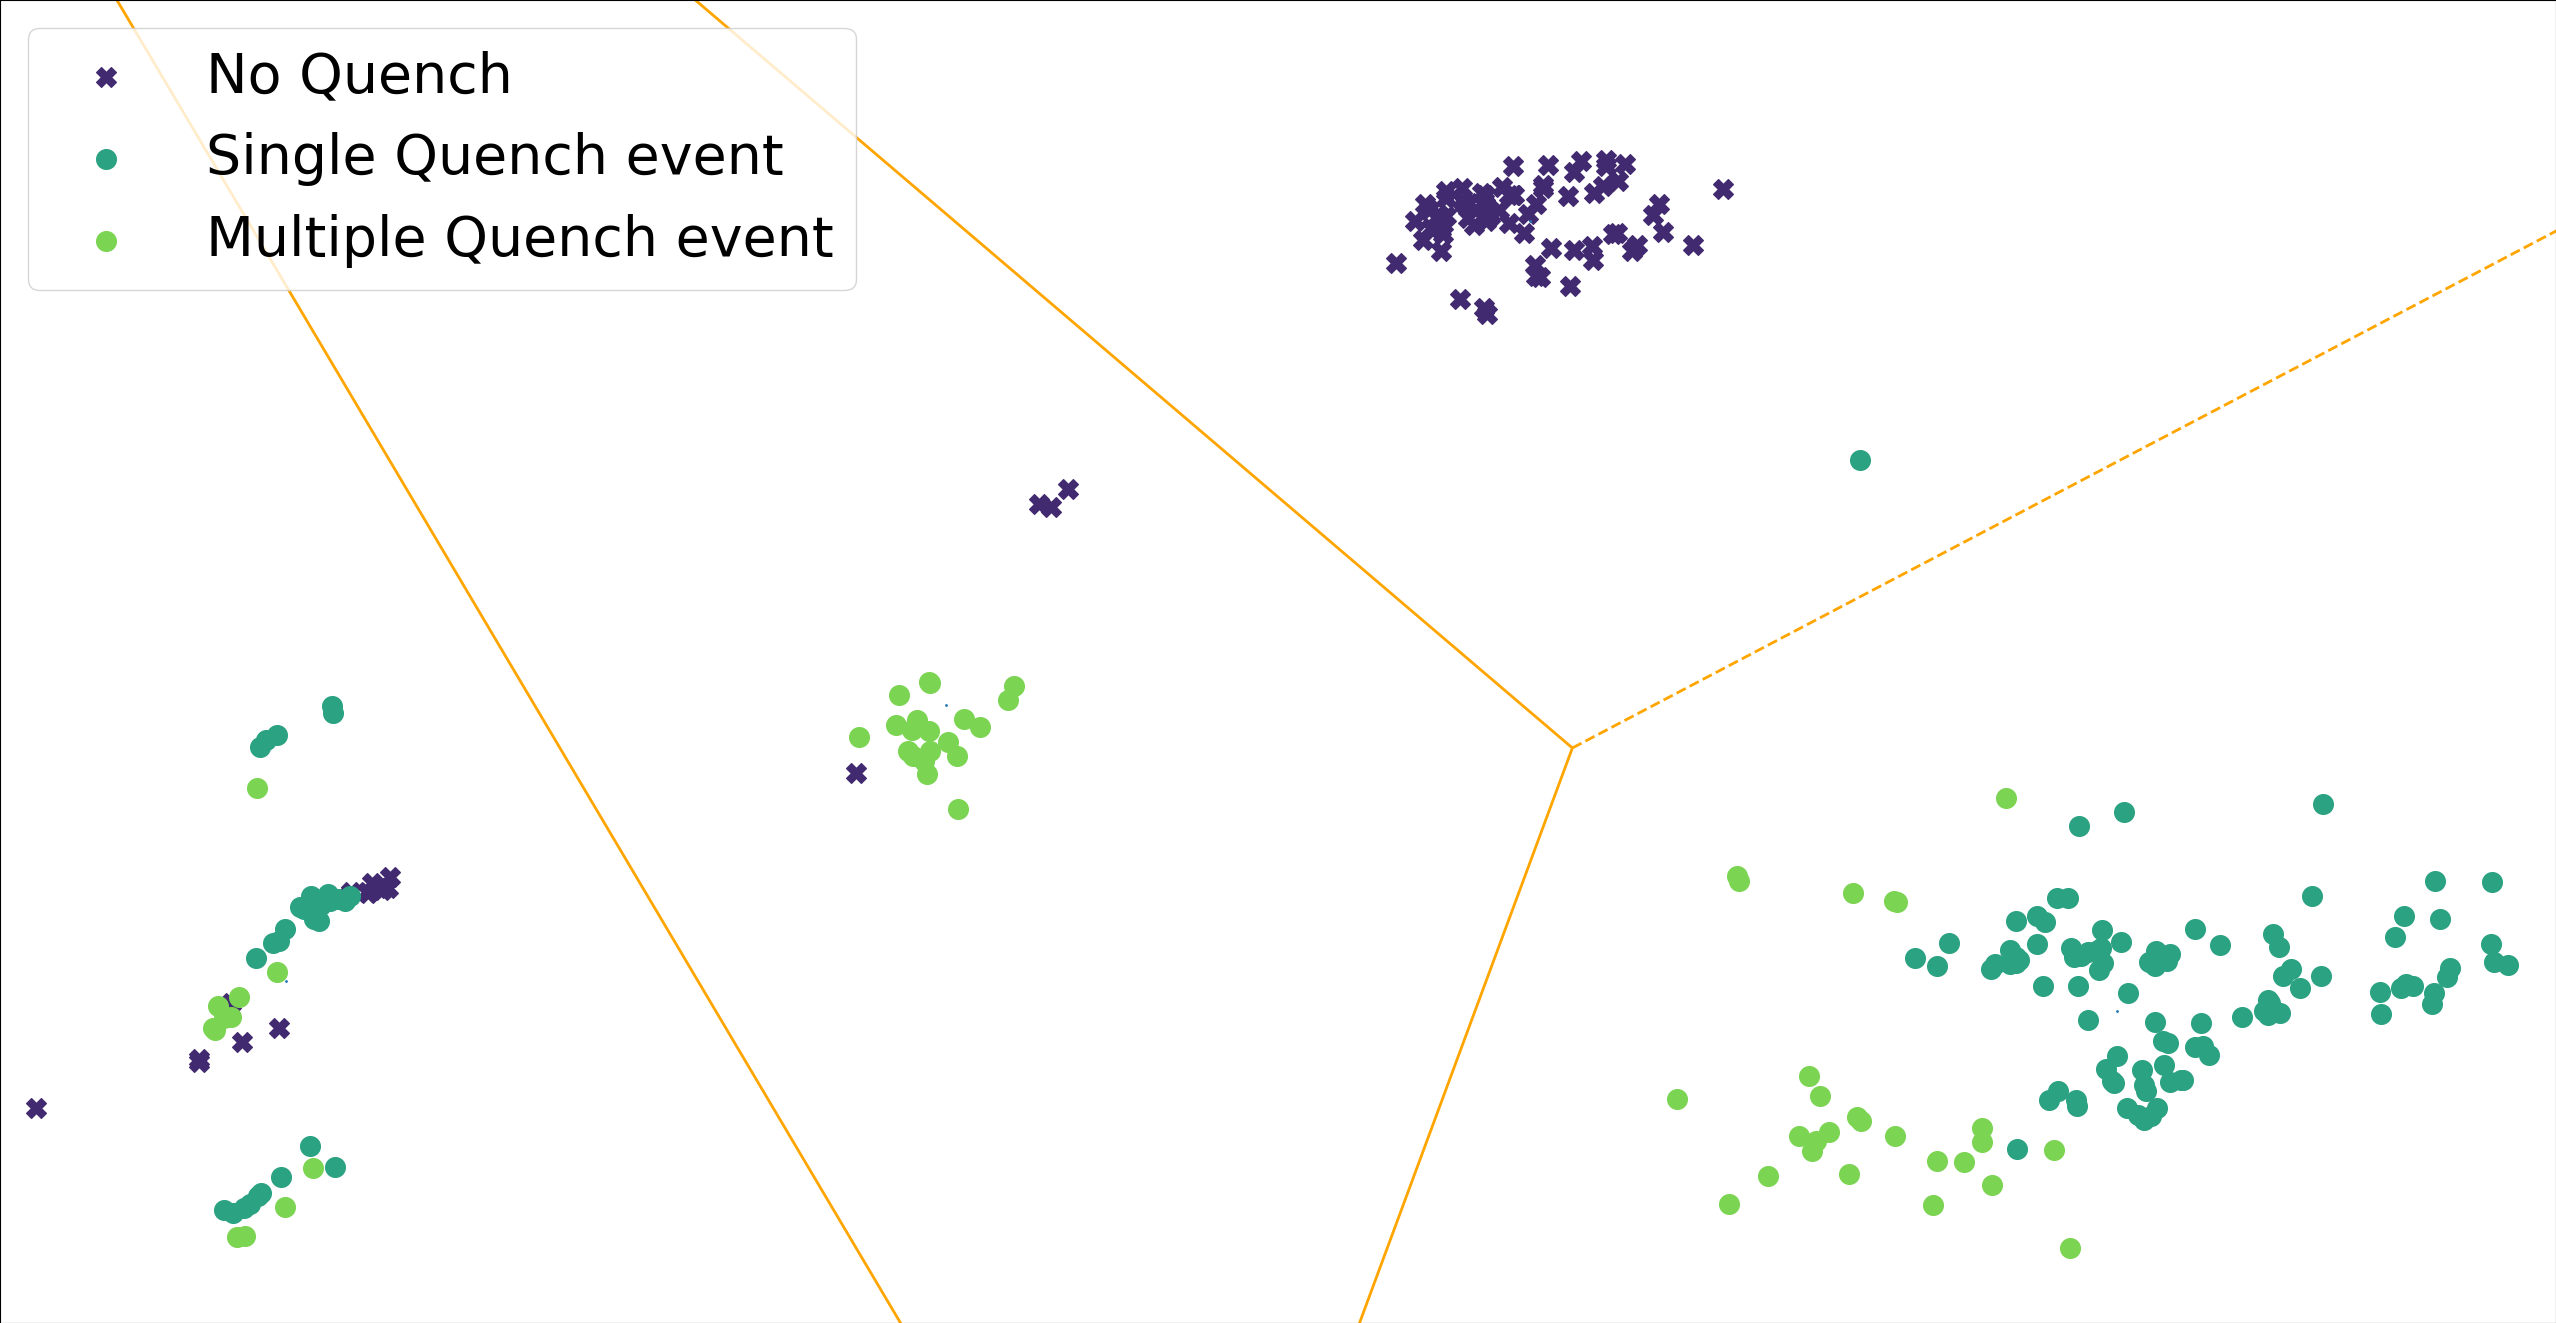
\includegraphics[width=\linewidth]{img/clustering_cnmod_qlp_4c.png}
		\caption{$4$-means clustering on \cnmod.}
	\end{subfigure}
	\caption{In the run of $4$-means clustering we decided to highlight the number of quenched
	samples arisen for every coil: $\{0, 1, \text{many}\}$} \label{fig:4-means-results}
\end{figure}

\Cref{fig:4-means-results} shows results of a $4$-means clustering run on both attributes, we chose
to label the samples based on the number of quenched coils $\{0, 1, \text{many}\}$. The orange lines
in the figure represent the cluster borders, if the line is solid then it has finite size, otherwise
it has infinite size. If we look at the results from the perspective of quench / no-quench
recognition, then the results for \an\ and \cnmod\ are very solid, since both present clusters
containing only one type of samples (the ones associated to no-quench and the ones associated to
measurements in which at least one coil quenched). If we look at this from a perspective of
identifying how many quench events were reported, per sample, then the $4$-way clustering is clearly
not enough, since almost all clusters have a high homogeneity of differently labelled samples.

According to the clustering-specific performance metrics (Silhouette and \textsc{db} scores, cfr.
\Cref{sec:kmeans}) using $4$ clusters represented for \an\ and \cnmod the best possible solution.
As we discussed above, though, this choice lead to suboptimal results, especially for \an. This
discrepancy is very likely due to the difference between the pattern identified by the algorithm
(looking to divide quenches from non-quenches) and our own expectation of what the result should
have been. We experimented with higher cluster counts, \cnmod\ gets visually worse: the
algorithm splits the cluster in the lower right region of \Cref{fig:cnmod-coilq-dist} (sub-figure (b)) in
different sub-clusters. A preliminary explanation for this behavior could be that it's trying to separate quench
events belonging to different coils (based on the per-coil quench visualization, see
\Cref{fig:cnmod-coilq-dist} (sub-figure (b))).

A run of $8$-means on \an\ generates clusters with a high level of purity. \Cref{fig:clustering-an} plots the result, the clusters identified by the algorithm are very clearly trying to separate three classes of samples: one associated to the magnet being in normal working condition, one associated to the magnet containing \emph{at most} one quenched coil, and finally, one associated to the magnet containing \emph{at least} one quenched coil.
\begin{figure}[!ht]
	\centering
	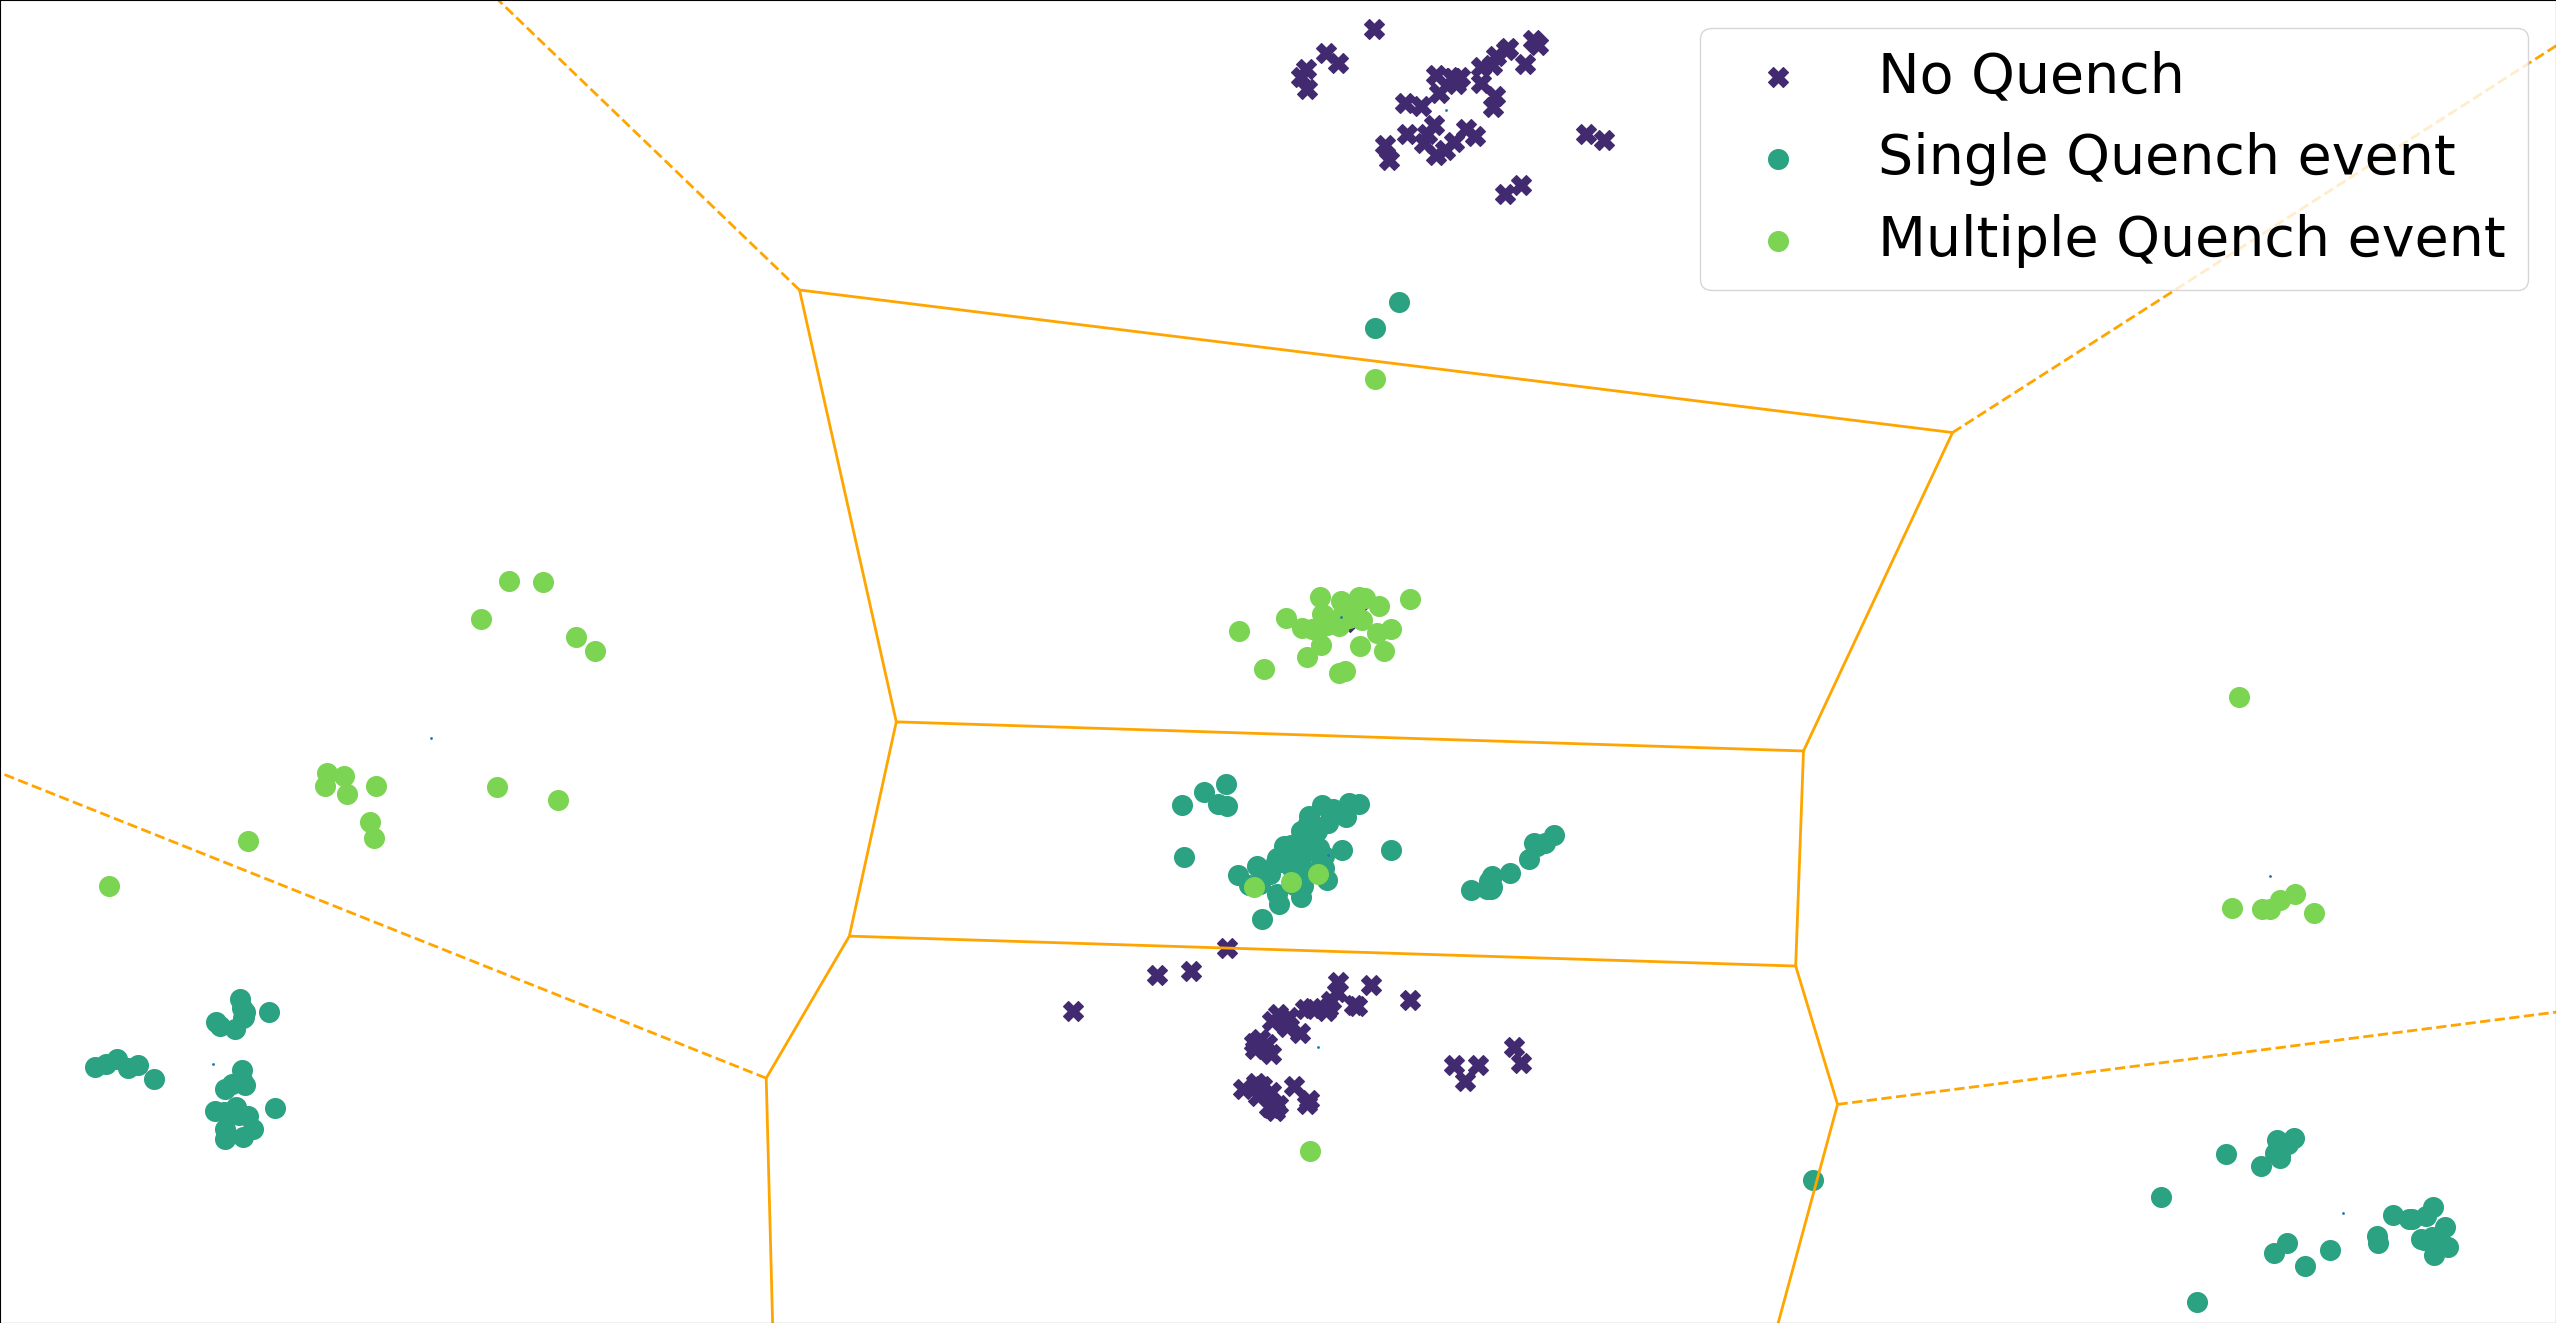
\includegraphics[width=0.6\linewidth]{img/clustering_an_qlp_8c.png}
	\caption{The results of a run of $8$-means on the sole attribute \an, after a round of \pca
		dimensionality reduction. As we can see all clusters have a high purity and only a handful of points have been misclassified.}\label{fig:clustering-an}
\end{figure}

Using clustering we achieved very interesting results and, while clustering alone might not be
enough as a classifier; we could still use it as a preprocessor for the models we saw in
\Cref{chp:qrp}. Alternatively, we could think of correcting misclassification errors by running an
instance of $k$-nn on top of $k$-means, in order to move misclissified points closer to where they
should be.
$k$-nn is the supervised alternative to $k$-means clustering. The algorithm is
non-parametric, as it does not assume a fixed form for the decision boundary and instead
relies directly on the training data, and instance-based, meaning that the outcome of the
algorithm depends directly from the training data, no pattern is abstracted from the samples
for later reuse. The classification outcome is computed by majority voting on the $k$ nearest
neighbours; the choice of the $k$ hyperparameter dictates how the algorithm behaves: a higher $k$
reduces the impact of noise by averaging over a larger number of neighbors, leading to a smoother
decision boundary~\cite{syriopoulos2025-knn}.

\section{Results}
After our brief exploration of the possibilities offered by clustering algorithms, we moved back to
supervised machine learning algorithms to solve \qlp. Our first approach was to do a na\"ive
extension of the models used to solve \qrp, to the multiclass-classification environment. We didn't
have high expectations for such models since the number of labels moved from $1$ to $4$ (see
\Cref{chp:problem}). Making the problem much more difficult than the original one.

\medskip

Using \dts\ to solve a multiclass-classification problem yielded more complicated estimators, with a
maximum depth $\in [5, 10]$, a high number of nodes, and an accuracy score close to $60 - 70\%$. This rough performance
number was obtained by micro averaging the accuracy of the classifier for every class; in other
words, the resulting metric is the average of the metric computed on each class, weighed on the cardinality of the class.

\medskip

Since the extension of \dts\ did not suit our expectations, we chose to change approach. Our new
idea was to turn \qlp\ into a binary classification problem. We first had to define a variation of
\qrp\ meant for single coils instead of the whole quadrupole. This variation, which we will call
\qrp-$i$, is capable of predicting, given the harmonic decomposition of the magnetic field, whether
a certain coil quenched $1$ or not $0$. The $4$ bit label vector associated to each sample for \qlp\
can be seen as $4$ different runs of \qrp-$i$, one for each coil ($i \in \{0, 1, 2, 3\}$). The model
solving \qlp\ will then be an aggregation of the $4$ models solving \qrp-$i$, performing
\emph{independently} of each other; the added complexity of having $4$ different models by design
made our decision process much more focused on model simplicity than it was when we faced \qrp.

\smallskip

We find important to highlight the fact that to solve \qlp we had to solve \qrp-$i$, instead of
reusing the best classifiers found for \qrp, because the function we found with \qrp links the
harmonic decomposition of magnetic field to quench events in a quadrupole. \qrp-$i$ uses the same
data to pose a different question, it might feel like a subtle difference, but it's an important
one.

In the following sections we will retrace our steps in \Cref{chp:qrp} and discuss the obtained results for the various models.

\subsection{Decision trees}
To keep the discussion concise, we will be describing the structure of the best models and
concentrate on the performance of the aggregate. Equation~\ref{eq:hamming} shows the metric we used to
compute the performance for the aggregate model, which contains one classifier per coil. We
denominated the metric 'Hamming score' ($\hs$ in the following), and it computes the Hamming
distance between the expected and the predicted label vectors, and then normalizes it.
\begin{equation}
	\label{eq:hamming}
	\hs = 1 - \frac{d_h(\hat{y}, y)}{4}
\end{equation}

\Cref{fig:bdts-qlp} visualizes the performance metrics obtained in the outer loop of a $5\times5$
fold \ncv\ for the best single tree trained on each coil. The metrics are quite close to each other,
with the only clear outlier being the model trained on coil $3$. Interestingly, while \bn was
supposed to be the better performer on coils $1$ and $3$, the best model was trained on a sub-view
of \cnmod, which was supposed to be the worst coil to use to gather any information about whether a
coil quenched or not in the magnet assembly (see \Cref{chp:problem} for more details).
\begin{figure}[!ht]
	\centering
	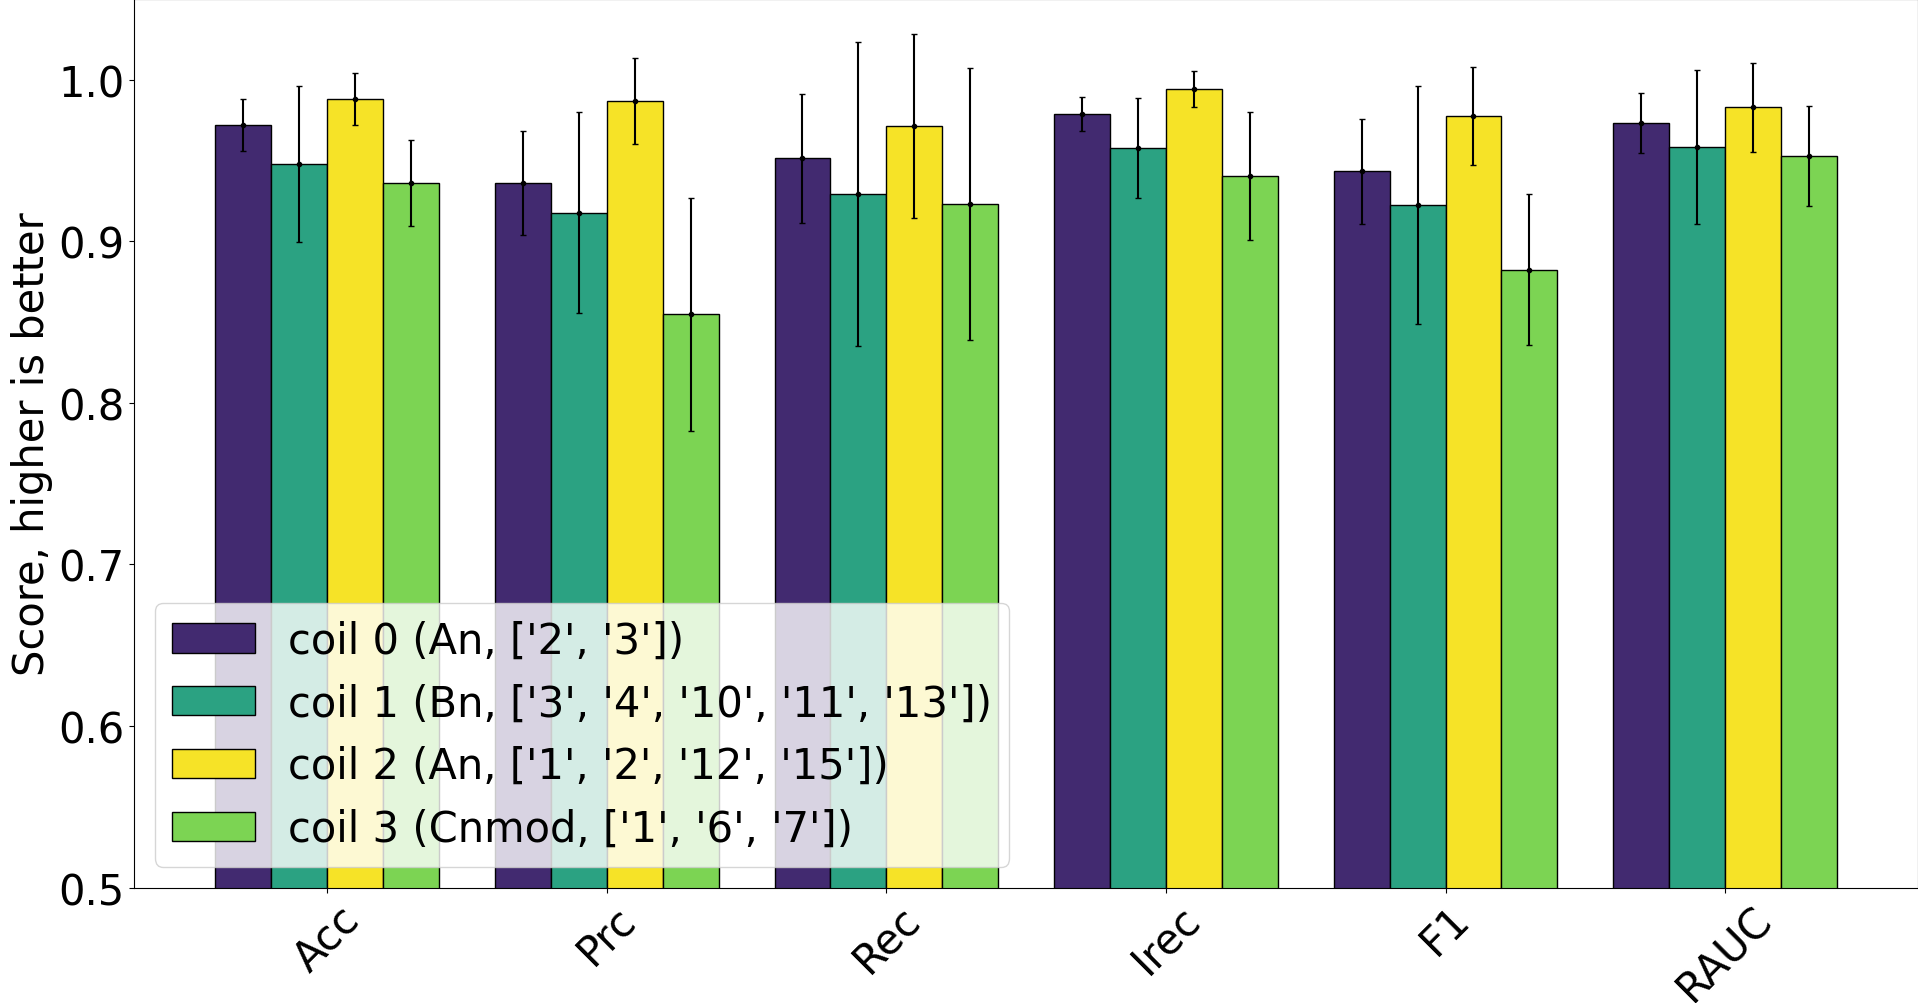
\includegraphics[width=0.7\linewidth]{img/best_dts_qlp.png}
	\caption{Comparing the performance of the best model built on every coil, independently of
		the dataset used.} \label{fig:bdts-qlp}
\end{figure}

We condensed the most important information in \Cref{tbl:tree-description}. All the trees have a
maximum depth of $5$ and the number of internal nodes and leaves is always acceptable. While the
trees built on \an\ remain on the smaller side, the trees used for coil $1$ and $3$ are larger (with
the one built on \cnmod\ being the more complex at $15$ total nodes).
\begin{table}[!ht]
	\caption{Description of the best \dt\ for every coil.}\label{tbl:tree-description}

	\bigskip
	\setlength{\tabcolsep}{6pt}
	\centering
	\begin{tabular}{lcccc}
		\toprule
		\textbf{}                           & \textbf{Coil 0}  & \textbf{Coil 1}          & \textbf{Coil 2}          & \textbf{Coil 3}
		\\
		\midrule
		\textsc{attribute}                  & \an              & \bn                      & \an                      & \cnmod                          \\
		\multirow{2}{*}{\textsc{harmonics}} & \an[2], \an[3]   & \bn[3], \bn[4], \bn[10], & \an[1], \an[2], \an[12], & \cnmod[1], \cnmod[6], \cnmod[7] \\
		                                    &
		                                    & \bn[11], \bn[13] & \an[15]                  &                                                            \\
		\textsc{depth}                      & 3                & 5
		                                    & 3                & 5                                                                                     \\
		\textsc{N internal nodes}           & 4                & 5
		                                    & 3                & 8                                                                                     \\
		\textsc{N leaves}                   & 5                & 6
		                                    & 4                & 7                                                                                     \\
		\textsc{N nodes}                    & 9                & 11
		                                    & 7                & 15                                                                                    \\
		\bottomrule
	\end{tabular}
\end{table}

\begin{figure}[!ht]
	\centering
	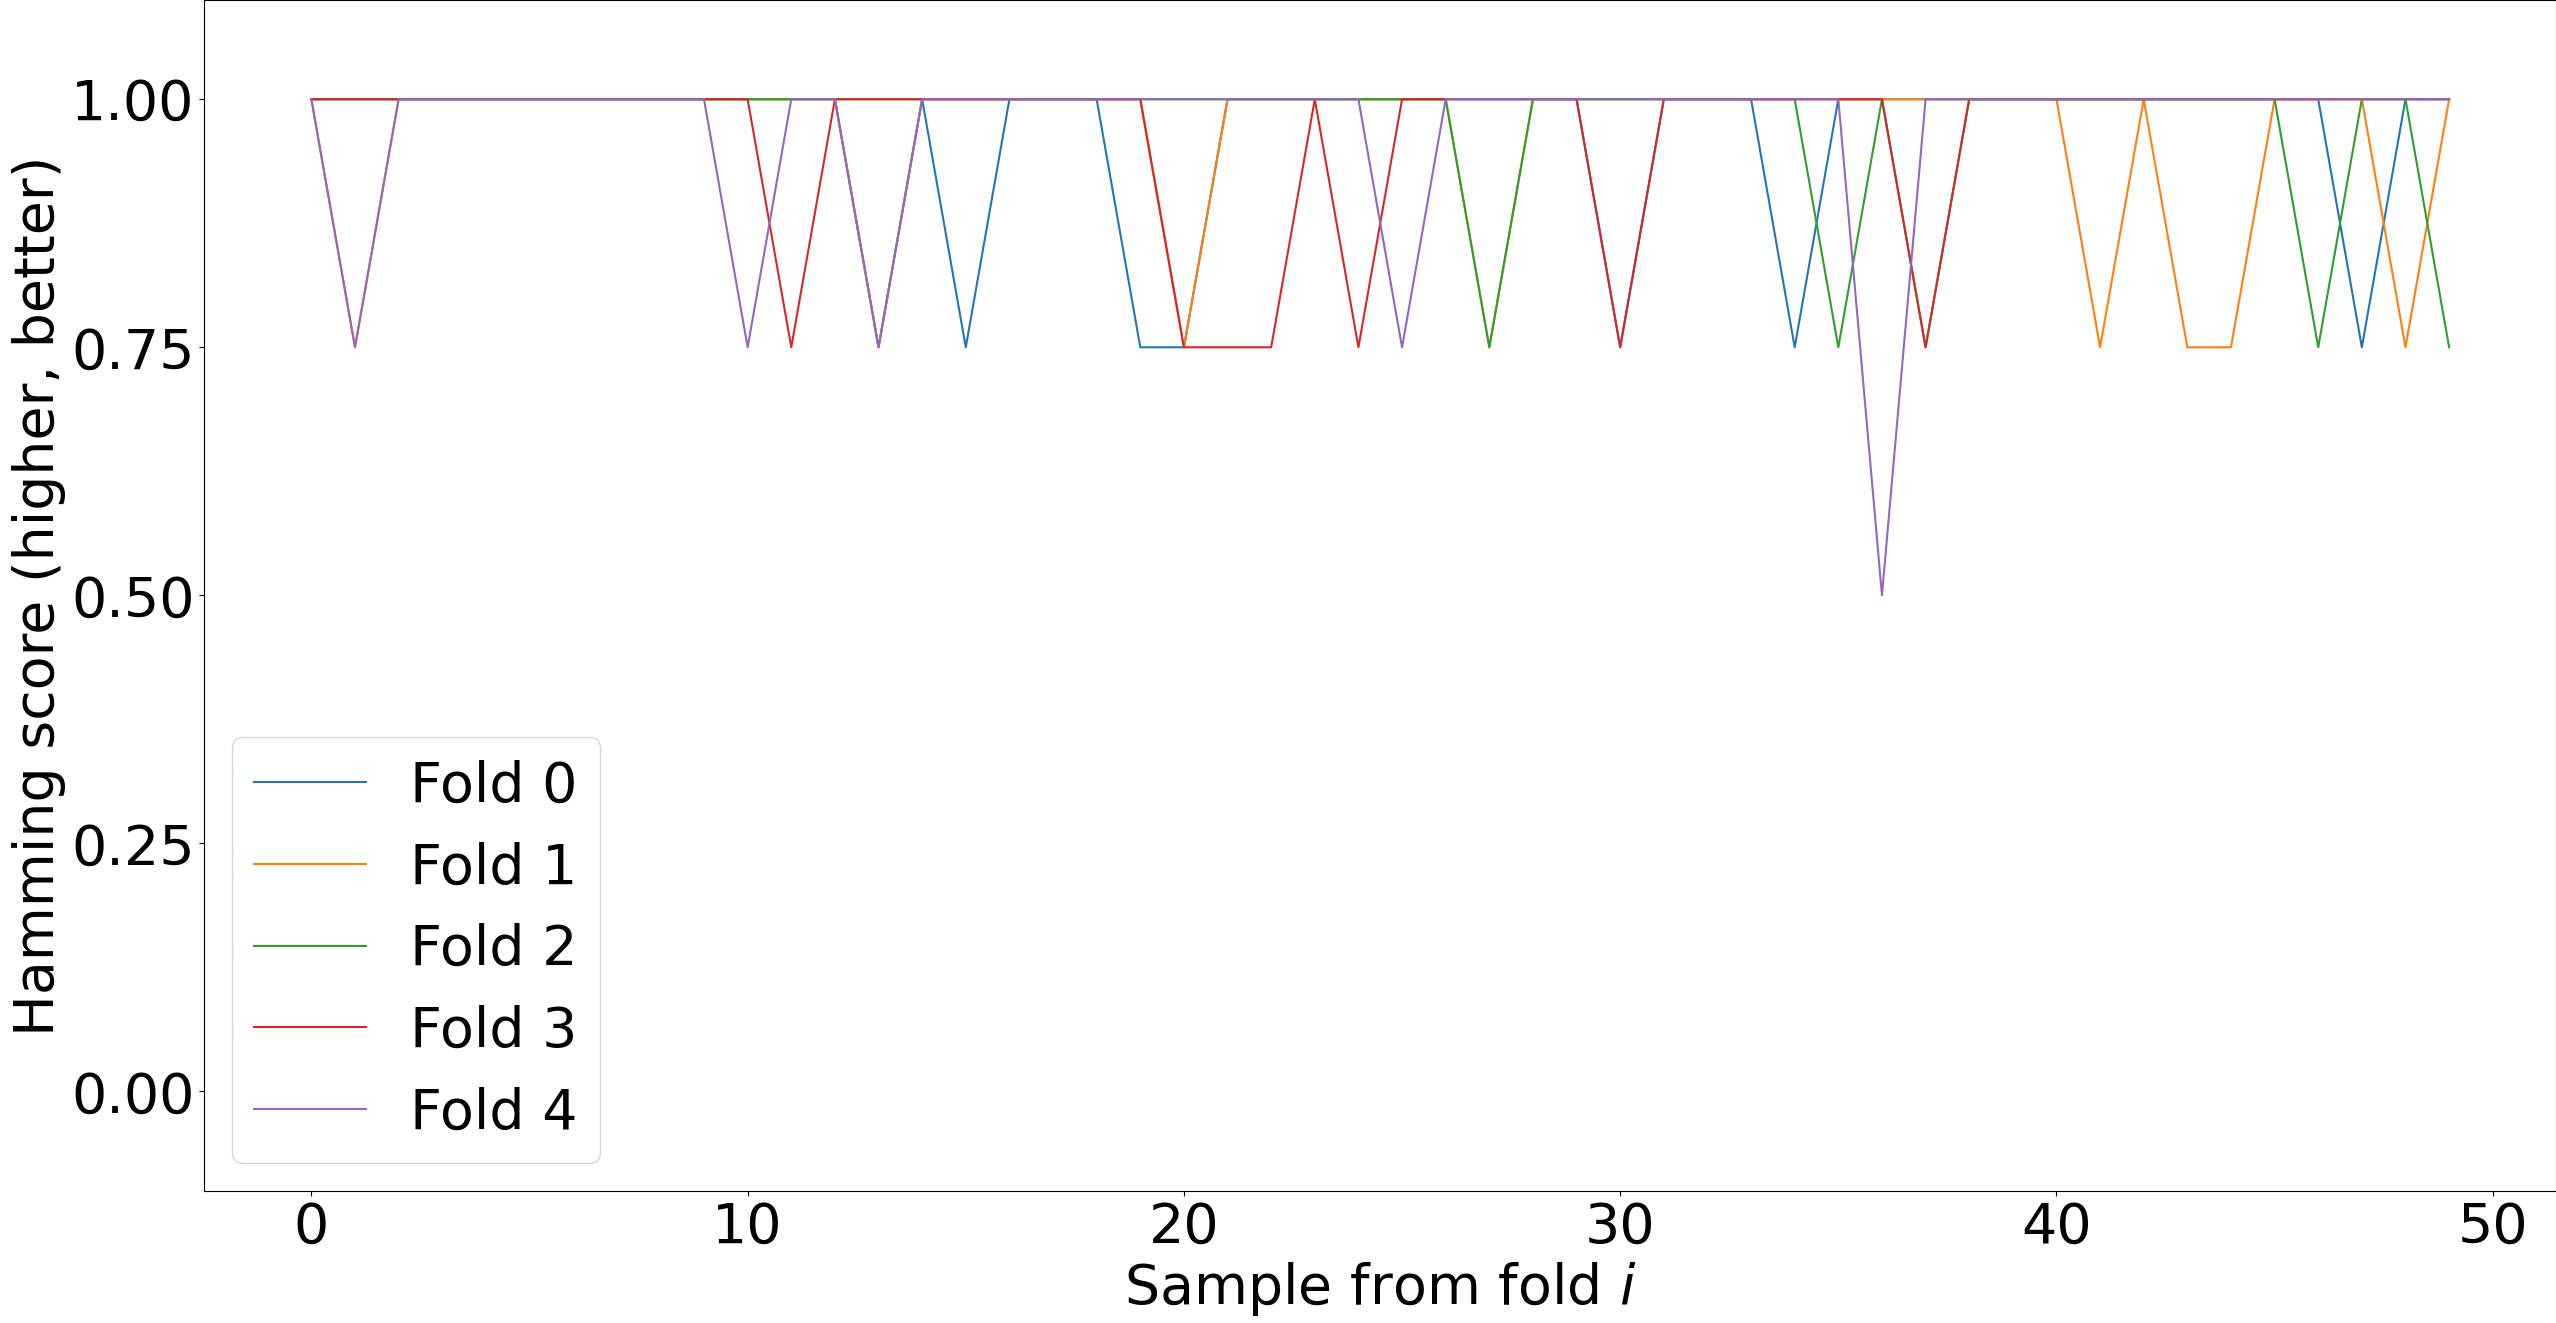
\includegraphics[width=0.7\linewidth]{img/best_dts_hs.png}
	\caption{The Hamming score computed on every fold (for the $50$ samples therein contained),
	the lower reaching is the line the lower is going to be the hamming score, and therefore the
	lower the accuracy.} \label{fig:dt-qlp-hs}
\end{figure}
In \Cref{fig:dt-qlp-hs}, we plotted the performance of the aggregate model, obtained as we
did when testing \tas\ for \qrp. The aggregate, built using the $4$ models described in
\Cref{tbl:tree-description}, was trained and tested using $5$-fold \cv, for each sample we:
\begin{inparaenum}[(i)]
\item predicted the value of the $4$ bits (using the $4$ different models),
\item put them in a vector and computed $\hs$,
\item plotted the point.
\end{inparaenum}
The ensemble makes at most $2$ errors, in most cases it just does one single error. By averaging the
performance over all folds, we get $0.967$ with a standard deviation of $0.051$. In
\Cref{tbl:dt-errors} we computed the number of errors done by every model on all the testing folds
to get a sense of which models made more errors. Since the models contained in the aggregate behave
independently, the higher the performance of the single model, the better the performance of the
final ensemble. A better model for the third coil would yield to much better performance on average.
\begin{table}[!ht]
	\caption{Each column contains the errors done by the model built on the specific coil for
	the specific testing fold, each fold contains $50$ samples.}\label{tbl:dt-errors}

	\bigskip
	\setlength{\tabcolsep}{6pt}
	\centering
	\begin{tabular}{ccccc}
		\toprule
		\textbf{}                     & \textbf{Coil 0}    & \textbf{Coil 1} & \textbf{Coil 2} & \textbf{Coil 3}
		\\
		\midrule
		\textsc{Fold 0}         & $2$           & $0$           & $0$            & $5$            \\
		\textsc{Fold 1}         & $2$		& $3$		& $0$            & $3$		  \\
		\textsc{Fold 2}		& $0$           & $0$		& $1$            & $4$            \\
		\textsc{Fold 3}         & $2$           & $2$ 		& $2$            & $1$            \\
		\textsc{Fold 4}         & $0$		& $3$           & $0$            & $3$            \\
		\midrule
		\textsc{total errors}	& $6$		& $8$		& $3$		& $16$
		\\
		\bottomrule
	\end{tabular}
\end{table}

Testing the performance of the aggregate on the final blind-test causes $4$ total errors ($4$ bits
were misclassified out of the $116$ total). If we average the Hamming score on the $29$ samples, we get higher
performance on average $0.966$, compared to training, and a standard deviation of $0.086$.

\subsection{Random forests}
Similarly to what we just did for \dts\ we also evaluated the performance of a model containing one forest per coil, we expected higher performance compared to the ones just obtained on \dts, at the expense of a lower explainability.

\begin{figure}[!ht]
	\centering
	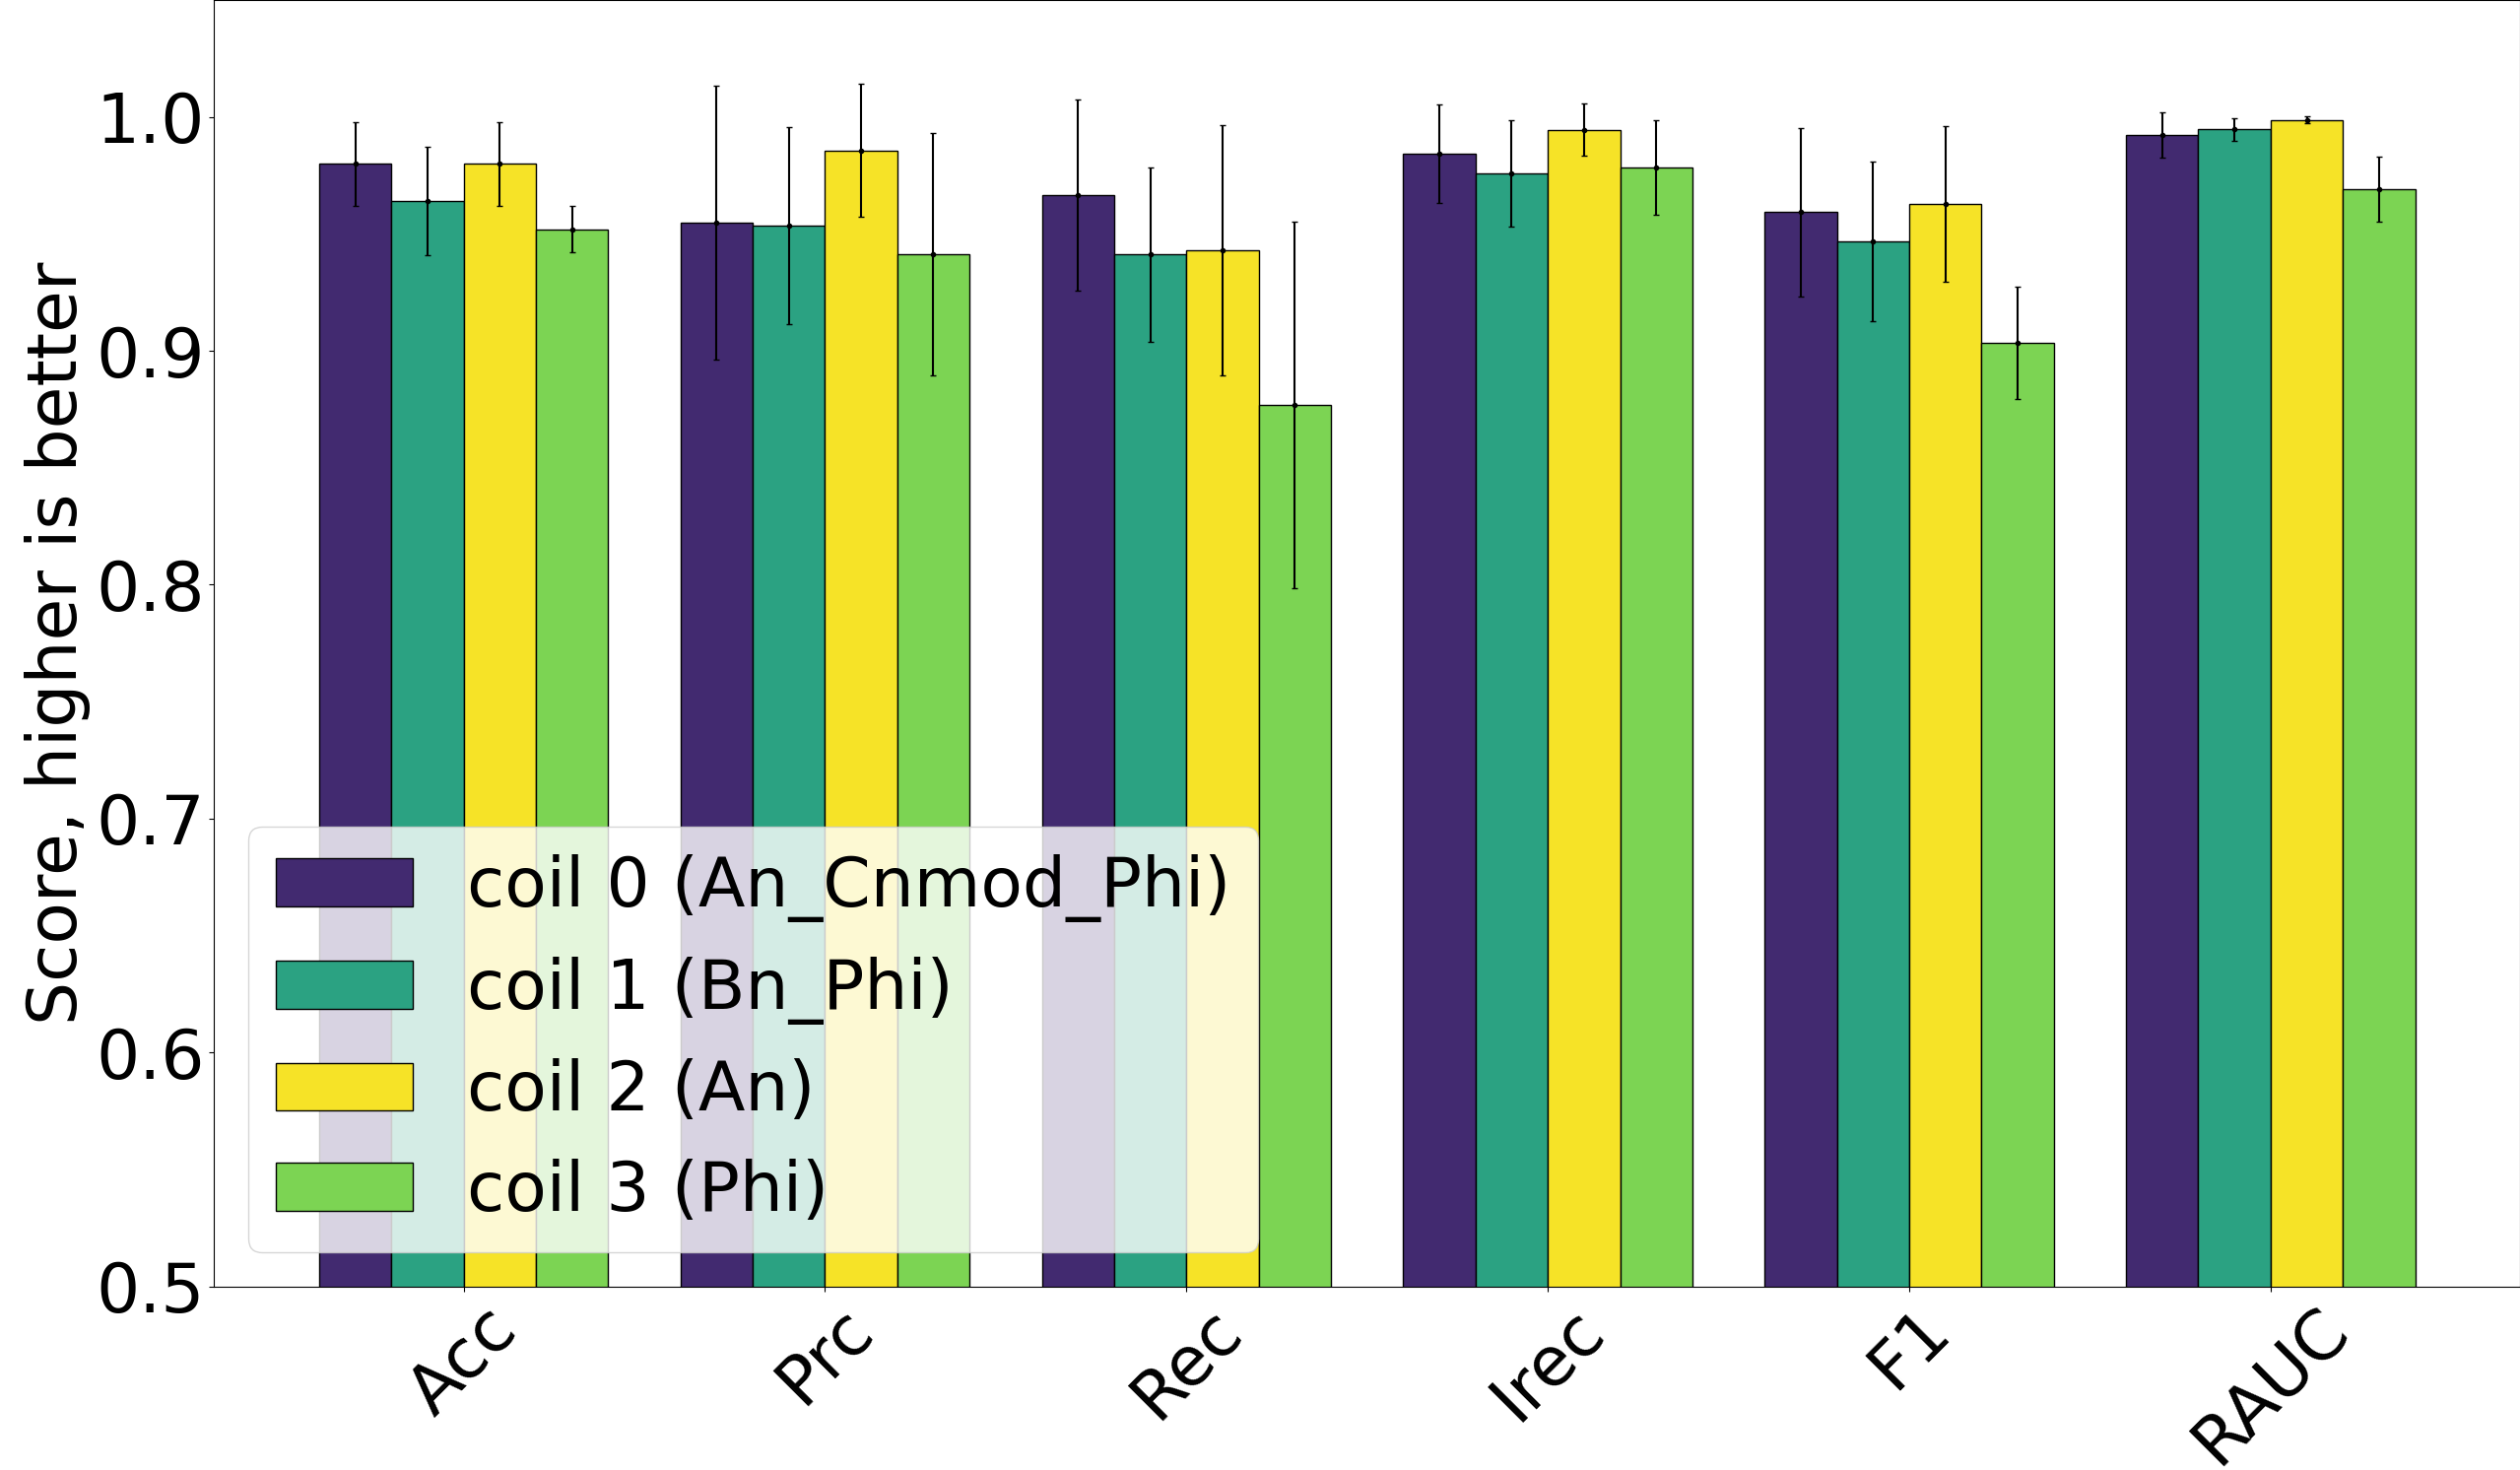
\includegraphics[width=0.7\linewidth]{img/best_rfs_qlp.png}
	\caption{The best random forest trained on a sub-view or mix of sub-views, for every coil.
		Since all models have been plotted without indicating the harmonic content, it means
		that they are using all the available harmonics.}\label{fig:brfs-qlp}
\end{figure}

\Cref{fig:brfs-qlp} shows the performance for the best \rfs\ built on a mix of different attributes
(each taken in its entirety). Performance metrics are better, but we are not far off from the
numbers obtained with \dts\ (see \Cref{fig:bdts-qlp}). The weakest learner, in this case as well, was the one built on coil $3$.

\Cref{tbl:forest-description} describes the four best forests. The depth, number of internal nodes and number of leaves has been
averaged on all the trees to give an idea of what the average tree would look like. We also included
the $5$ most important harmonics for each forest, to have a sense of which features counted the
most in the estimator. A couple of aspects stood up to us, as explained here below:
\begin{itemize}
	\item The forests are very complicated, contain many trees which can be quite deep. The
		most complicated of them is the one constructed on coil $3$, which reaches an
		average number of $15$ nodes for $10$ trees.
	\item The model dedicated to coil $0$ is trained on a dataset using attributes \an, \cnmod\ and
		\phin. Despite this, the $5$ most important harmonics are all taken from \an.
\end{itemize}
The excessive complexity of these models lead us to abandon the model early because the slight
performance increase over \dts\ wasn't really worth the extreme complexity jump.
\begin{table}[!ht]
	\caption{Description of the best \rf\ for every coil.}\label{tbl:forest-description}

	\setlength{\tabcolsep}{6pt}
	\centering
	\begin{tabular}{lcccc}
		\toprule
		\textbf{}                     & \textbf{Coil 0}    & \textbf{Coil 1} & \textbf{Coil 2} & \textbf{Coil 3}
		\\
		\midrule
		\textsc{attribute}            & \an, \cnmod, \phin & \bn, \phin
		                              & \an                & \phin                                               \\
			\multirow{2}{*}{\textsc{harmonics}} & \an[3], \an[10], \an[11]   & \phin[6],
			\bn[13], \bn[3], & \an[3], \an[7], \an[13], & \phin[6], \phin[11], \phin[13] \\
							    & \an[7], \an[9]
							    & \bn[9], \bn[5] & \an[10], \an[12]
							    &\phin[1], \phin[10]                                                            \\
		\textsc{N estimators}         & $5$                & $10$            & $10$            & $10$            \\
		\textsc{avg. depth}            & $2.6$              & $3.7$
		                              & $3  $              & $4  $                                               \\
		\textsc{avg. N int. nodes} & $2.6$              & $4.4$
		                              & $3.5$              & $7.9$                                               \\
		\textsc{avg. N leaves}         & $4.5$              & $5.4$
		                              & $4.9$              & $8.9$                                               \\
		\bottomrule
	\end{tabular}
\end{table}

\subsubsection{Support Vector Classifiers}
We used \svcs\ as our benchmark model for \qlp\ as well. In \Cref{fig:bsvcs-qlp} we plotted the
performance metrics for the best \svc\ trained on every coil.
\begin{figure}[!ht]
	\centering
	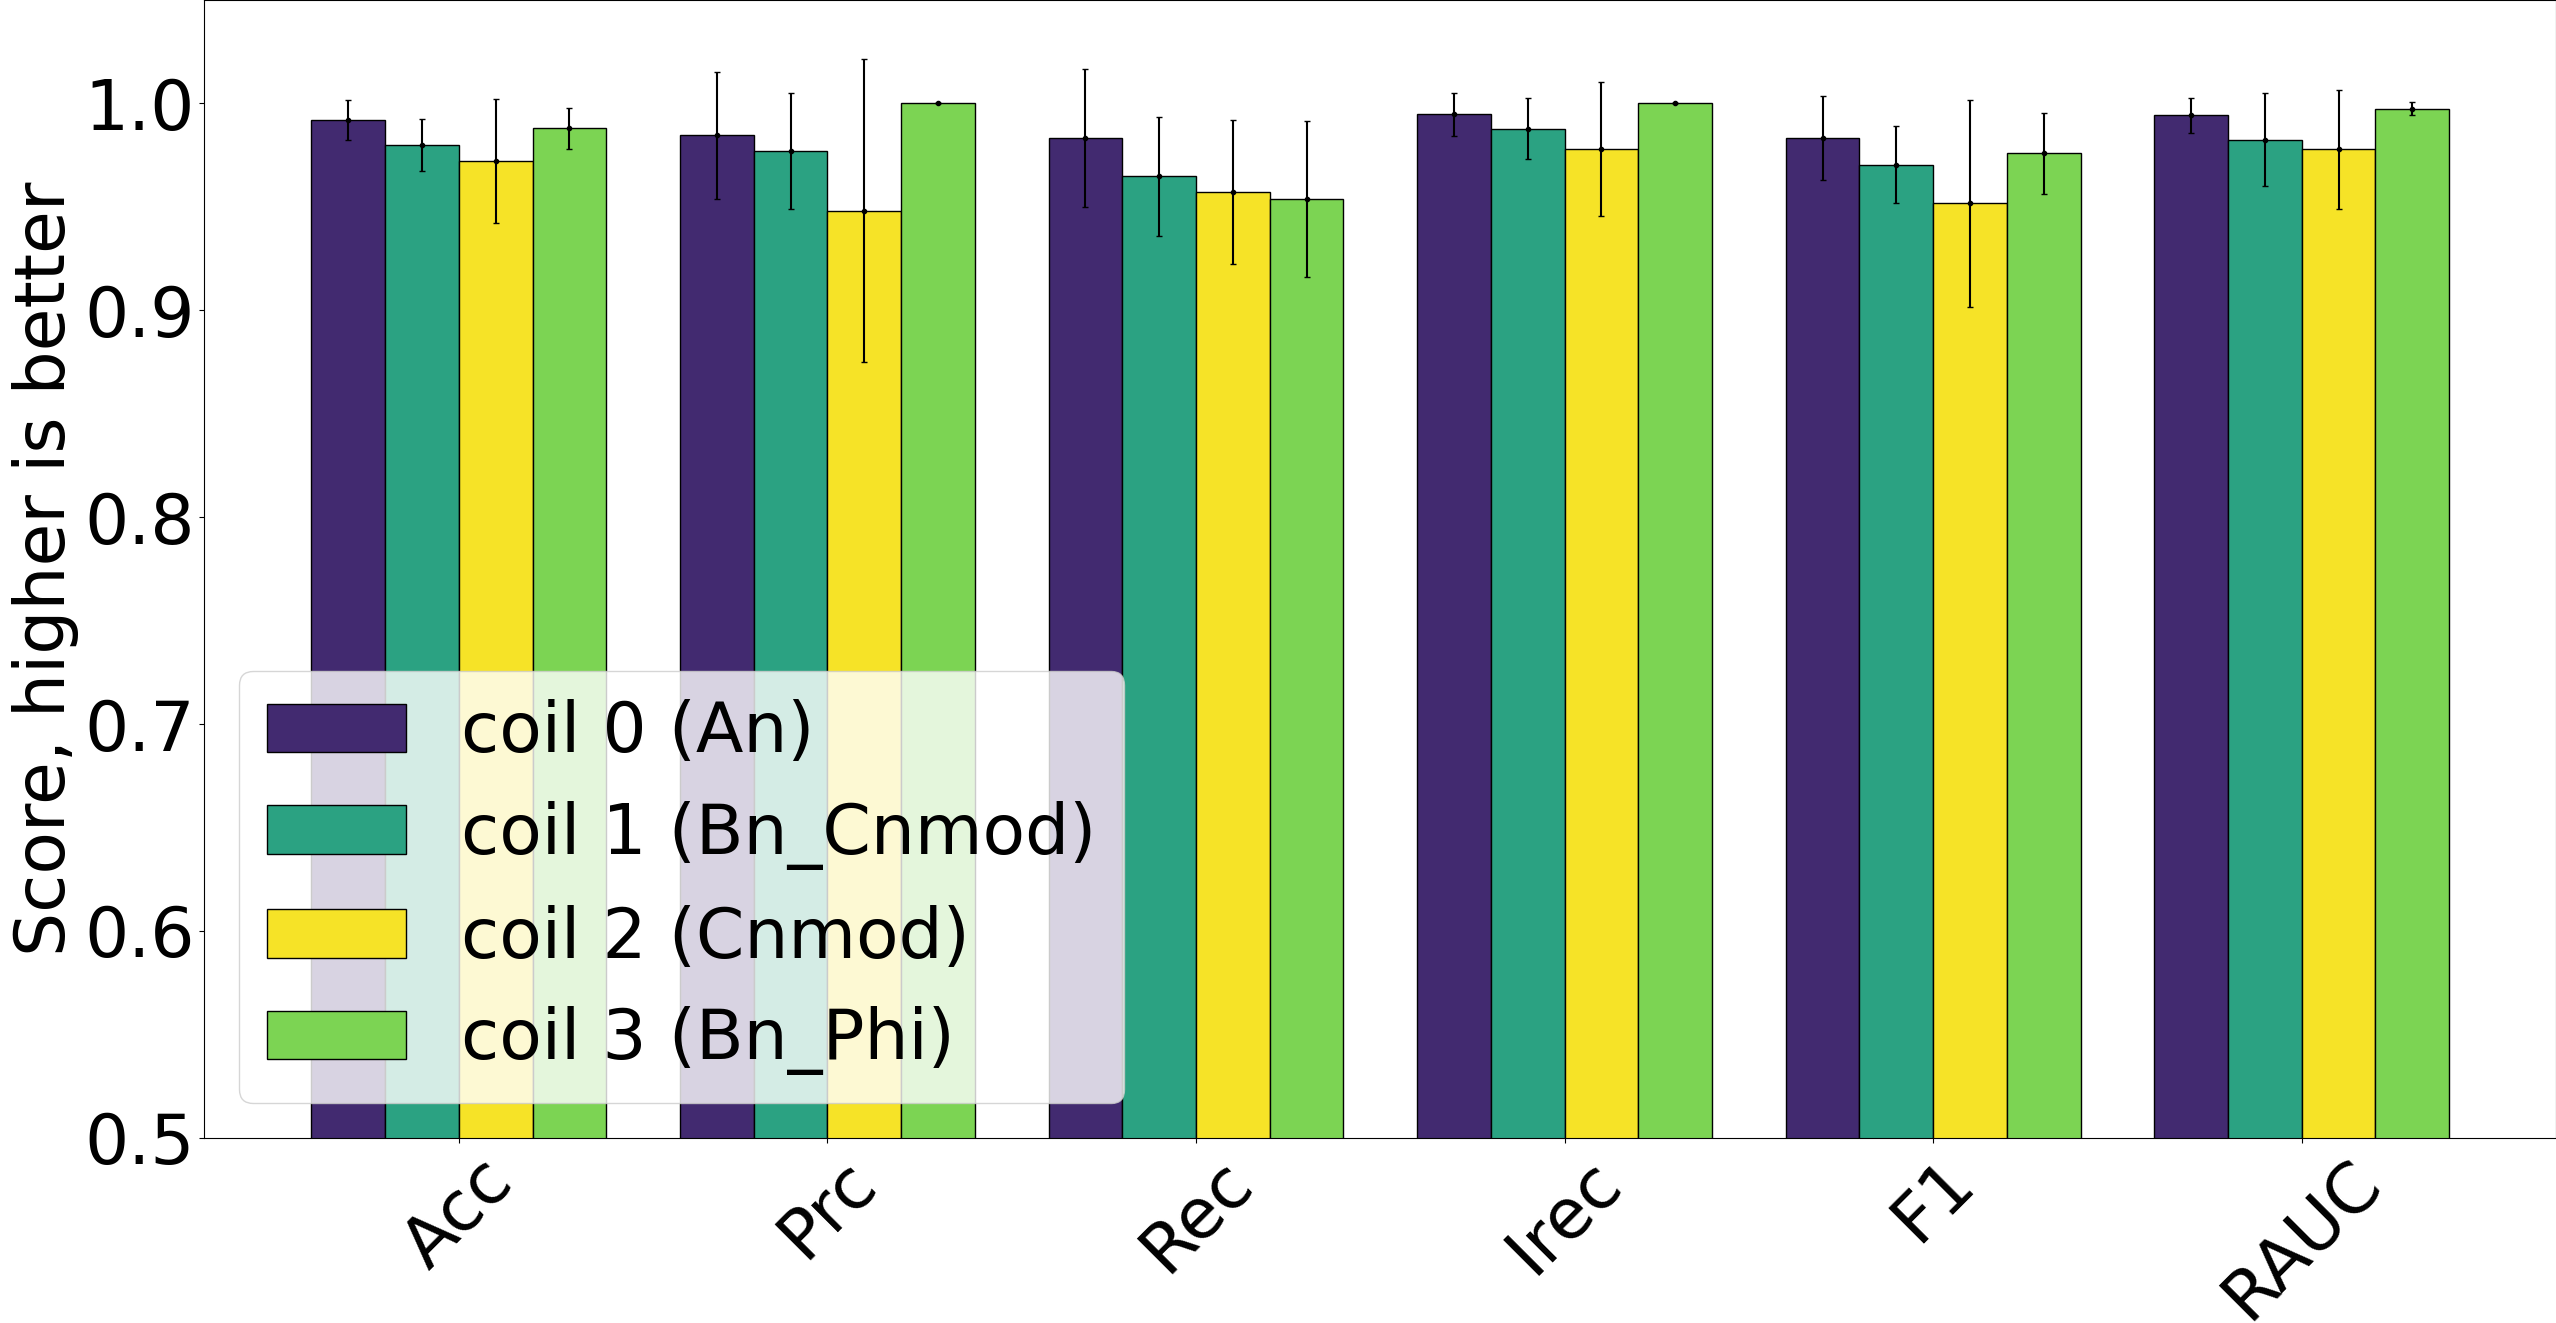
\includegraphics[width=0.7\textwidth]{img/best_svcs_qlp.png}
	\caption{Performance metrics for the best \svcs\ trained on every coil, all attributes
		have been taken with their full harmonic content.} \label{fig:bsvcs-qlp}
\end{figure}
There are a couple of very interesting takeaways.
\begin{itemize}
	\item The best \svc\ trained on coil $0$ is based on attribute \an. This is exactly what we
	      expected since the very beginning of this chapter.
	\item The best models for coils $1$ and $3$, were trained on \bn\ and another dataset (\cnmod\ for $1$ and \phin\ for $3$). This is interesting for two reasons:
	      \begin{inparaenum}[(i)]
	      \item the correlation between \bn\ and the labels of coils $1$ and $3$ is very strong,
		      (see \Cref{fig:bn-lcorr-qlp}), and we expected to see it put to use in these
		      cases,
	      \item the \svc\ trained on the sole \bn\ performed worse than the alternatives. This
		      lead us to believe that, like in the case of \qrp, \bn\ alone doesn't contain
		      enough information.
	      \end{inparaenum}
	\item Interestingly, while \cnmod\ didn't perform well enough in our tests on \dts\ for coil
	      $2$; the \svc\ trained on it was chosen over alternative trained on \an.
\end{itemize}
\begin{figure}[!ht]
	\centering
	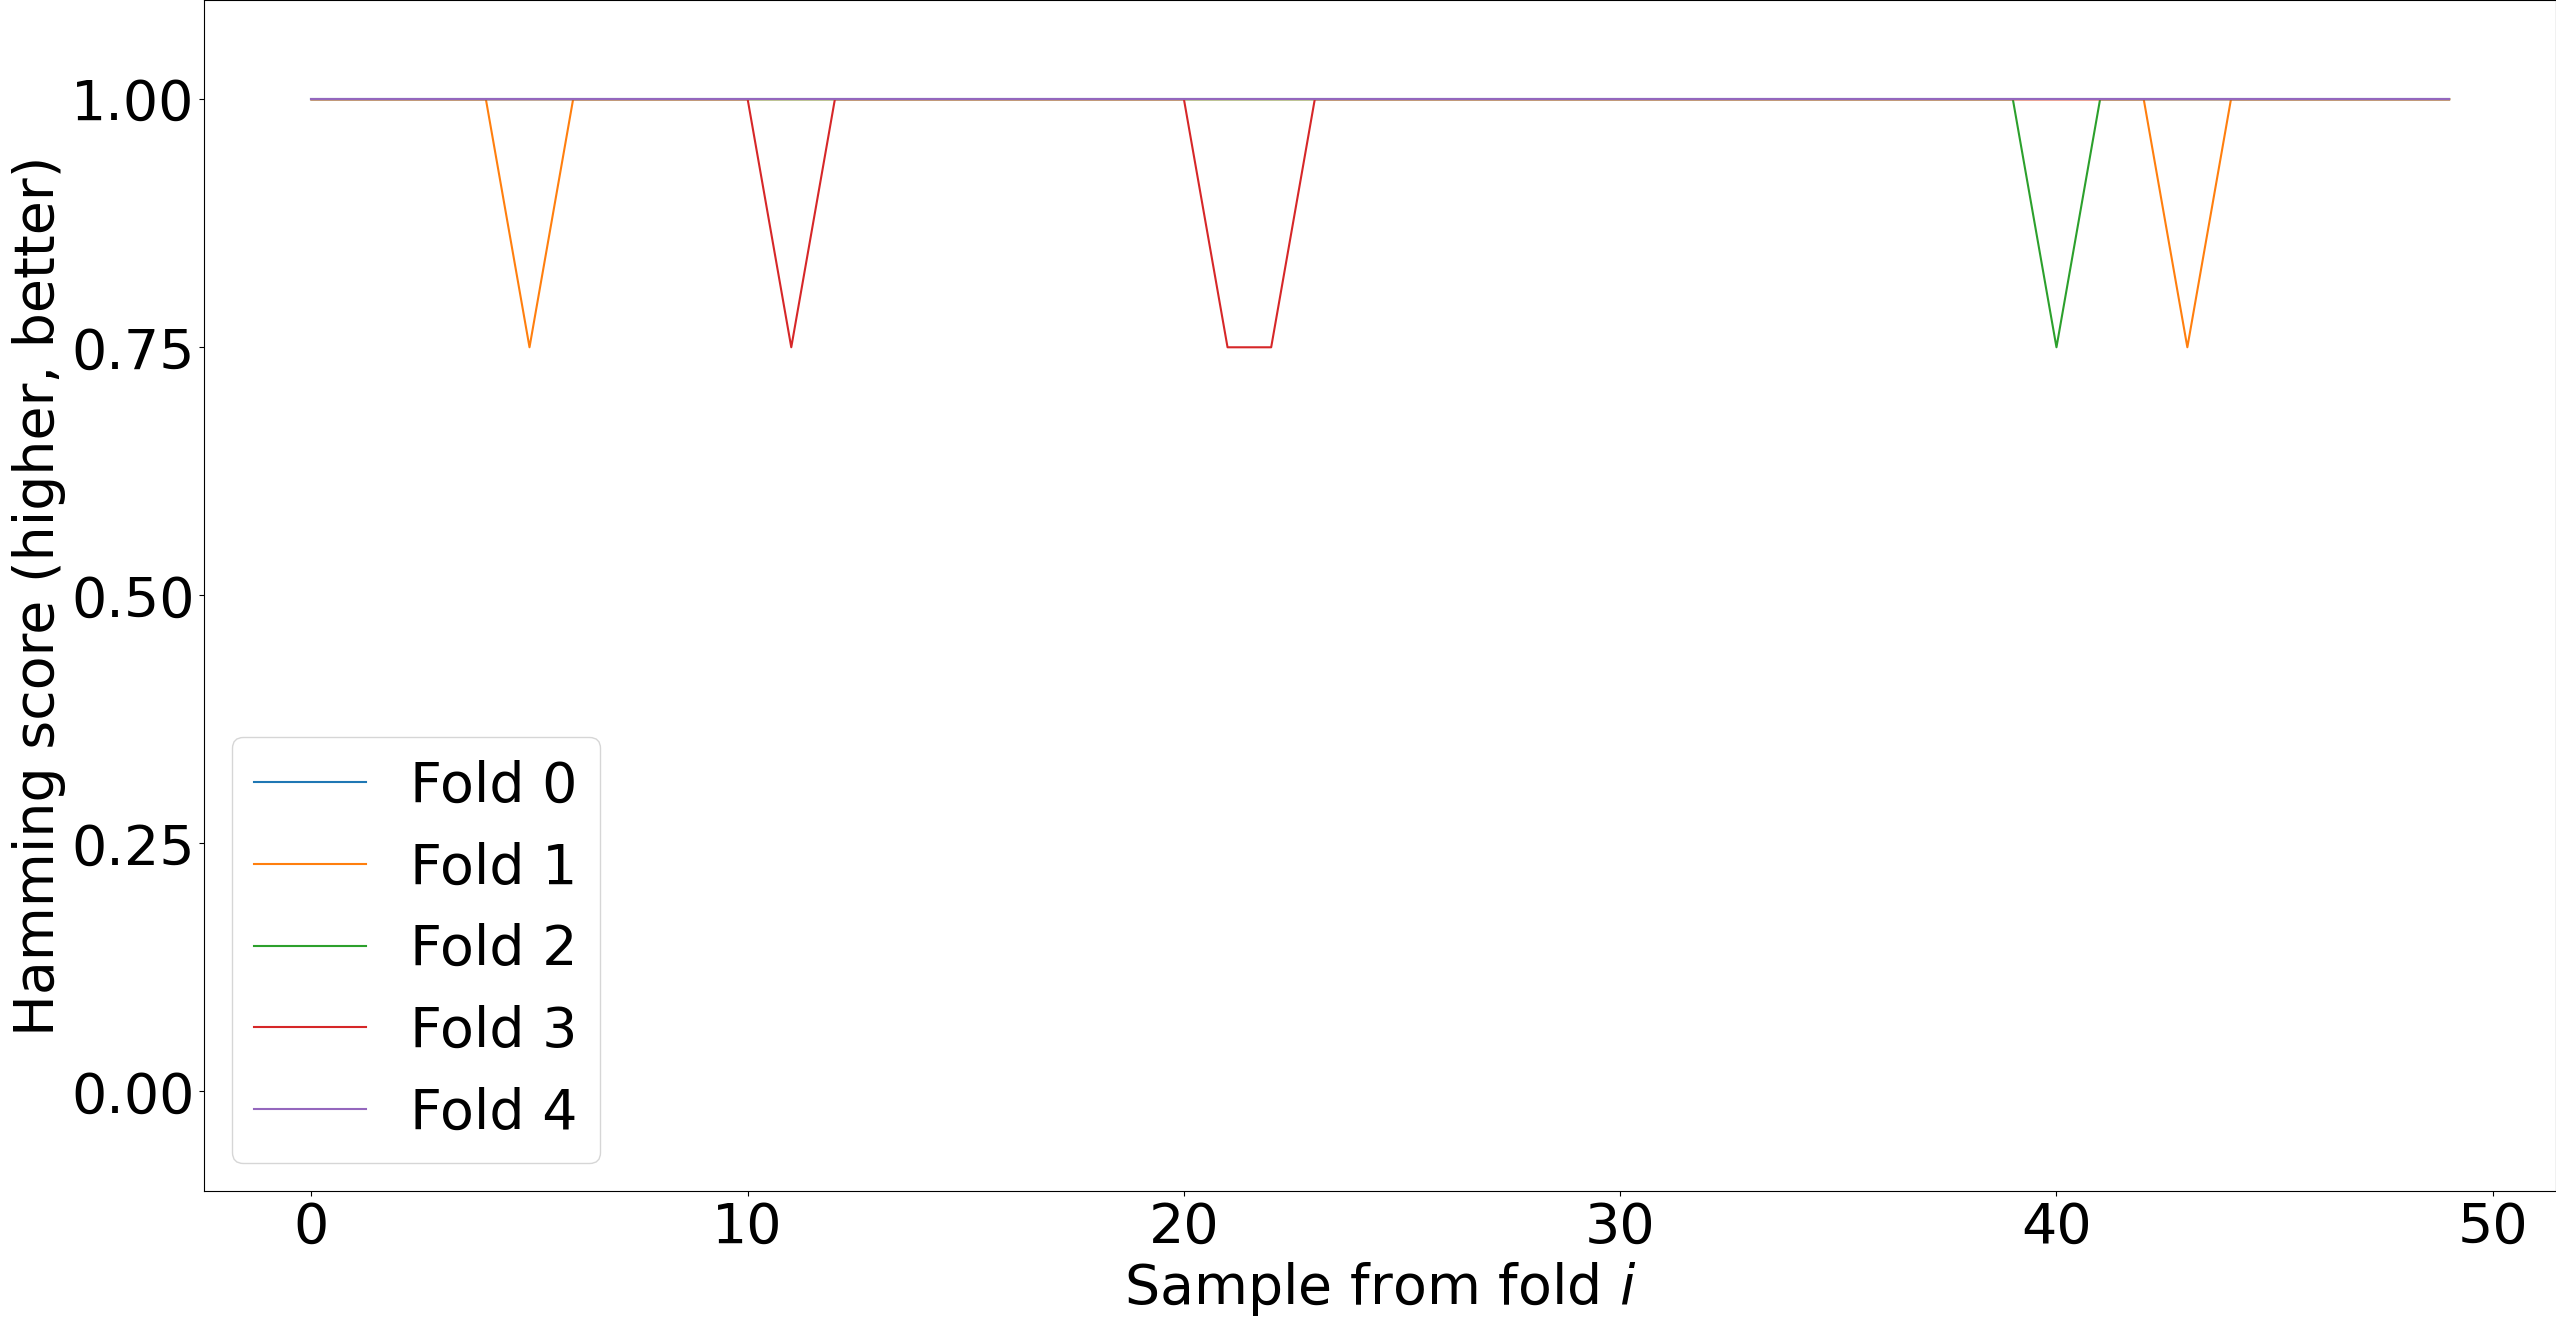
\includegraphics[width=0.7\linewidth]{img/svc_qlp_hs.png}
	\caption{The Hamming score computed on every fold (for the $50$ samples therein contained),
	fir \svcs. The lower reaching is the line the lower is going to be the accuracy.}
	\label{fig:svc-qlp-hs}
\end{figure}
\begin{table}[!ht]
	\setlength{\tabcolsep}{6pt}
	\centering
	\begin{tabular}{ccccc}
		\toprule
		\textbf{}                     & \textbf{Coil 0}    & \textbf{Coil 1} & \textbf{Coil 2} & \textbf{Coil 3}
		\\
		\midrule
		\textsc{Fold 0}         & $0$           & $0$           & $0$            & $0$            \\
		\textsc{Fold 1}         & $0$		& $0$		& $2$            & $0$		  \\
		\textsc{Fold 2}		& $0$           & $0$		& $0$            & $1$            \\
		\textsc{Fold 3}         & $1$           & $1$ 		& $1$            & $0$            \\
		\textsc{Fold 4}         & $0$		& $0$           & $0$            & $0$            \\
		\midrule
		\textsc{total errors}	& $1$		& $1$		& $3$		& $1$
		\\
		\bottomrule
	\end{tabular}
	\caption{Each column contains the errors done by the model built on the specific coil for the specific testing fold, each fold contains 50 samples.}\label{tbl:svc-err}
\end{table}

In \Cref{fig:svc-qlp-hs} we plotted $\hs$ for every point in the $5$ cross validation folds, as we
did for \dts. In \Cref{tbl:svc-err} we indicated the error done by each model on the $5$ folds and
the total for each model. Clearly, all \svcs\ have very high performance, doing just a handful of
errors in total. The average $\hs$ score for the \svc\ is $0.994$ and its standard deviation is $0.006$.




